%% Garcia's latex template for Activities Drescriptive Memorial Report
%% Version 0.2
%% (c) 2015 Vinicius Cardoso Garcia (vcg@cin.ufpe.br)
%%
%% This document is based on latex template from Prof. Daniel Cunha.
%%
%% Reference commands. Use the following commands to make references in your
%% text:
%%          \figref  -- for Figure reference
%%          \tabref  -- for Table reference
%%          \eqnref  -- for equation reference
%%          \chapref -- for chapter reference
%%          \secref  -- for section reference
%%          \appref  -- for appendix reference
%%          \axiref  -- for axiom reference
%%          \conjref -- for conjecture reference
%%          \defref  -- for definition reference
%%          \lemref  -- for lemma reference
%%          \theoref -- for theorem reference
%%          \corref  -- for corollary reference
%%          \propref -- for proprosition reference
%%          \pgref   -- for page reference
%%
%%          Example: See \chapref{chap:introduction}
%%%%%%%%%%%%%%%%%%%%%%%%%%%%%%%%%%%%%%%%%%%%%%%%%%%%%%%%%%%%%%%%%%%%%%%%%%%%%%%

\documentclass[a4paper,oneside,10pt]{article}

\usepackage{graphicx}
\usepackage{amsmath,amstext,amssymb,amsfonts}
\usepackage[none]{hyphenat}
\usepackage{fancyhdr}
\usepackage{cite}
\usepackage{indentfirst}
%\usepackage{path}
\usepackage[usenames, dvipsnames]{color}

\usepackage{pdfsync}
\usepackage{url}
\usepackage{setspace}
\usepackage[latin1,utf8]{inputenc}
\usepackage[T1]{fontenc}
\usepackage{colortbl}
\newcommand{\SetRowColor}[1]{\noalign{\gdef\RowColorName{#1}}\rowcolor{\RowColorName}}

\definecolor{MyRed}{rgb}{1,0.2,0.1}
\definecolor{light-gray}{gray}{0.95}
\definecolor{gray}{gray}{0.6}

\usepackage{booktabs}
\usepackage{ctable}
\usepackage{setspace}
\usepackage[multidot]{grffile}
\usepackage[final]{pdfpages}

\usepackage{titlesec}

\usepackage[toc,page]{appendix}
\newcommand{\appref}[1]{\@appendixname~\ref{#1}\xspace}
%\usepackage{xifthen}

\usepackage[bookmarks,colorlinks,pdfpagelabels,
pdftitle={Memorial Descritivo de Atividades}, pdfauthor={Nome Completo Autor},
pdfsubject={Solicita\c{c}\~{a}o de progresss\~{a}o funcional docente de Adjunto N\'{\i}vel 3 para Adjunto N\'{\i}vel 4 apresentada \`{a} Comiss\~{a}o de Avalia\c{c}\~{a}o de Progress\~{a}o Horizontal do Centro de Inform\'{a}tica da Universidade Federal de Pernambuco.},
pdfcreator={André Monteiro Paschoal}, pdfkeywords={Professor, Doutor, IFGW, UNICAMP, Docente}]{hyperref}

\newcommand{\otoprule}{\midrule[\heavyrulewidth]}

% Defini\c{c}\~{a}o de margens
\setlength{\textwidth}{16cm} %
\setlength{\textheight}{23cm} %
\setlength{\oddsidemargin}{0cm} %
\setlength{\evensidemargin}{0cm} %
\setlength{\topmargin}{0cm}

\renewcommand{\abstractname}{Resumo}
\renewcommand{\contentsname}{\'{I}ndice Anal\'{\i}tico}
\renewcommand{\refname}{Refer\^{e}ncias}
\renewcommand{\appendixname}{Ap\^{e}ndice}
\renewcommand{\tablename}{Tabela}

%% Formata\c{c}\~{a}o do cabe\c{c}alho e rodap\'{e}
\lhead{\footnotesize Memorial Descritivo de Atividades} %
\rhead{\footnotesize \emph{André Monteiro Paschoal}} %
\chead{} %
\cfoot{} %
\lfoot{\footnotesize\nouppercase\leftmark} %
\rfoot{\bfseries\thepage}
\renewcommand{\footrulewidth}{0.1pt}

% Comando para inserir n\'{u}mero de documento
\newcounter{document}%[section]
\setcounter{document}{0}
\renewcommand\theenumi{\arabic{section}.\arabic{enumi}}
\newcommand\Doc{{\addtocounter{document}{1}\mbox{\sffamily\bfseries [Doc. \arabic{document}]}}}

% Comando para repetir um n\'{u}mero de documento j\'{a} citado
% \mbox{\sffamily{\bfseries{[Doc. XX]}}}

%% Alternativa na edi\c{c}\~{a}o dos comandos.
%% Comando para inserir n\'{u}mero de documento
% \newcommand\thedocument{%
%    \ifthenelse{\arabic{subsection}=0}
%      {\thesection.\arabic{document}}
%      {\thesubsection.\arabic{document}}}
% \newcounter{document}[section]
% \setcounter{document}{0}
% \renewcommand\theenumi{\arabic{section}.\arabic{enumi}}
% \ifthenelse{\arabic{subsection} = 0}{\newcommand\Doc{{\stepcounter{document}\bfseries [Doc. \arabic{section}.\arabic{document}]}}}{\newcommand\Doc{{\stepcounter{document}\bfseries [Doc. \arabic{section}.\arabic{subsection}.\arabic{document}]}}}
% %\newcommand\Doc{{\addtocounter{document}{1}\mbox{\bfseries [Doc. \arabic{document}]}}}


% Ambiente para centralizar vertical
\newenvironment{vcenterpage}
     {\newpage\vspace*{\fill}}
     {\vspace*{\fill}\par\pagebreak}

\sloppy

\pagestyle{fancy}

\setcounter{secnumdepth}{4}

\begin{document}

\begin{titlepage}

\vspace{-5.0cm}

\begin{figure}[!htb]
 \centering{
\includegraphics[width=0.8\textwidth]{Figuras/ifgw.jpg}}
 \label{fig:IFGW_logo}
\end{figure}

\begin{center}
\vspace{1cm}
%{\huge \textsf{Solicita\c{c}\~{a}o de Progress\~{a}o Funcional Docente}} \\[1cm]
\rule{1.0\textwidth}{1pt} \\ [0.5cm]
{\Huge \textbf{\textsf{Memorial Descritivo de Atividades}}} \\
\rule{1.0\textwidth}{1pt} \\
\vspace{2cm}

\doublespacing
{\Large \textsf{Solicita\c{c}\~{a}o de contratação para o cargo de de \textbf{Professor Doutor - MS-3.1} apresentada ao Instituto de Física "Gleb Wataghin", da Universidade de Campinas}}\\
\vspace{1.5cm}
{\LARGE \textsf{Solicitante: \textbf{XXX XXX XXXX}}}\\
\vspace{0.5cm}
%{\Large \textsf{SIAPE: \textbf{1807586}}} \\
%\vspace{0.5cm}
%{\Large \textsf{Per\'{\i}odo: \textbf{20/08/2014 - 19/08/2016}}} \\

\vspace{2.0cm}

\normalsize \textsf{Abril de 2022}

\end{center}
\thispagestyle{empty}
\end{titlepage}


\tableofcontents
%\include{Lista_Anexos} \cleartooddpage[\thispagestyle{empty}]

%%%%%%%%%%%%%%%%%%%%%%%%%%%%%%%%%%%%%%%%%%%%%%%%%%%%%%%%%%%%%%%%%%%%%%%%%%%%%%%
% APRESENTA\c{C}\~{A}O
%%%%%%%%%%%%%%%%%%%%%%%%%%%%%%%%%%%%%%%%%%%%%%%%%%%%%%%%%%%%%%%%%%%%%%%%%%%%%%%

\newpage
\section*{Apresenta\c{c}\~{a}o}
\vspace{0.3cm}

\begin{onehalfspace}

Memorial apresentado por \textbf{Autor}, para concurso de Professor Doutor MS - 3.1 junto ao Instituto de Física "Gleb Wataghin" da Universidade de Campinas (UNICAMP), para avalia\c{c}\~{a}o de desempenho acad\^{e}mico.
O presente memorial relata as atividades desempenhadas no per\'{\i}odo de \textbf{Fevereiro de 2008 até Abril de 2022}. Os documentos comprobat\'{o}rios referenciados neste memorial est\~{a}o organizados em volumes anexos devidamente numerados. 
Por fim, os Anexos que se referem a artigos publicados em confer\^{e}ncias e peri\'{o}dicos cont\'{e}m apenas a primeira p\'{a}gina do trabalho e o email informando a aceita\c{c}\~{a}o do trabalho para publica\c{c}\~{a}o (quando pertinente).

\end{onehalfspace}

%%%%%%%%%%%%%%%%%%%%%%%%%%%%%%%%%%%%%%%%%%%%%%%%%%%%%%%%%%%%%%%%%%%%%%%%%%%%%%%
% APRESENTA\c{C}\~{A}O DO CANDIDATO
%%%%%%%%%%%%%%%%%%%%%%%%%%%%%%%%%%%%%%%%%%%%%%%%%%%%%%%%%%%%%%%%%%%%%%%%%%%%%%%

\newpage
\section{Trajet\'{o}ria acad\^{e}mica}
\vspace{0.3cm}

\begin{onehalfspace}

Incluir aqui um texto explicando sua trajetória acadêmica e explicando suas motivações pessoais.

\end{onehalfspace}

%%%%%%%%%%%%%%%%%%%%%%%%%%%%%%%%%%%%%%%%%%%%%%%%%%%%%%%%%%%%%%%%%%%%%%%%%%%%%%%
% Grupo 1 - Identificação do Candidato
%%%%%%%%%%%%%%%%%%%%%%%%%%%%%%%%%%%%%%%%%%%%%%%%%%%%%%%%%%%%%%%%%%%%%%%%%%%%%%%
\newpage
\section{Identificação}

\begin{itemize}
        \large{\item \textbf{Nome COmpleto Autor}}
        \item Filiação: \newline
        Pai: Nome do pai. \newline
        Mãe: Nome da mãe.
        \item Data e local de nascimento
        \item Cargo atual na carreira universitária: incluir a posição que se encontra, o local onde se encontra e fonte de financiamento (bolsa).
        \item Residente no endereço tal.
        \item Telefone para contato: XXXXXXX
        \item E-mail para contato: XXXXX
        \item Membro das Seguintes Sociedades:
        \begin{itemize}
                \item International Society of Magnetic Resonance in Medicine (ISMRM).
                \item European Society of Magnetic Resonance in Medicine and Biology (ESMRMB).
        \end{itemize} 
        
\end{itemize}

%%%%%%%%%%%%%%%%%%%%%%%%%%%%%%%%%%%%%%%%%%%%%%%%%%%%%%%%%%%%%%%%%%%%%%%%%%%%%%%
% Grupo 2 - Formação do Candidato
%%%%%%%%%%%%%%%%%%%%%%%%%%%%%%%%%%%%%%%%%%%%%%%%%%%%%%%%%%%%%%%%%%%%%%%%%%%%%%%
\newpage
\section{Formação}
\large{
\begin{enumerate}
        \item Graduação:
        \begin{itemize}
                \item Graduação em \textbf{Curso de graduação}, obtida junto ao Local Onde Se Graduou no ano de XXXX \mbox{\sffamily{\bfseries{[Doc. \ref{diplomas:graduacao}]}}} \\
                \item Iniciação científica no laboratório XXXX no ano XXXX. %\mbox{\sffamily{\bfseries{[Doc. \ref{diplomas:IC}]}}} \\ 
        \end{itemize}

        \item Pós-graduação:
        \begin{itemize}
                \item Mestre em Ciências com grau obtido no programa de XXXX, junto ao XXXXX no ano de XXXX. %\mbox{\sffamily{\bfseries{[Doc. \ref{diplomas:mestrado}]}}} \\
                \item Doutor em Ciências com grau obtido no programa de Física Aplicada à Medicina e Biologia (FAMB), junto ao Departamento de Física da Faculdade de Filosofia, Ciências e Letras de Ribeirão Preto (FFCLRP) da Universidade de São Paulo (USP) no ano de 2020. %\mbox{\sffamily{\bfseries{[Doc. \ref{diplomas:doutorado}]}}} \\
                \item Pós-doutorando junto à XXXXX de Fevereiro à Dezembro de 2020. %\mbox{\sffamily{\bfseries{[Doc. \ref{diplomas:posdoc1}]}}}\\
                \item Estágio de pesquisador junto ao Instituto XXXX desde Janeiro de 2021 até o presente momento. %\mbox{\sffamily{\bfseries{[Doc. \ref{diplomas:posdoc2}]}}} \\
        \end{itemize}

        \item Participação em projetos de pesquisa:
        \begin{itemize}
                \item Pesquisador associado no projeto FAPESP número XXXXXXX %\mbox{\sffamily{\bfseries{[Doc. \ref{certificados:fapesp_regular2019}]}}} \\
                \item Membro colaborador da iniciativa internacional \textit{Open Science Iniciative for Perfusion Imaging} (OSIPI - \url{https://osipi.org/}), da qual é atualmente o líder 
        da \textit{Task Force 6.1 - ASL Challenges:} \url{https://osipi.org/task-force-6-1/}.
        \end{itemize}

        \item Atuação profissional:
        \begin{itemize}
                \item Estagiário na empresa XXXX no período de 08 de fevereiro à 07 de dezembro de 2012 %\mbox{\sffamily{\bfseries{[Doc. \ref{declaracao:SAPRA}]}}}
        \end{itemize}

        \item Formação complementar:
        \begin{itemize}
                \item XXXX \\
        \end{itemize}

        \item Idiomas:
        \begin{itemize}
                \item Inglês: compreende bem; lê bem; escreve bem; fala bem.
                \item Português: compreende bem; lê bem; escreve bem; fala bem.
        \end{itemize}
\end{enumerate}}

%%%%%%%%%%%%%%%%%%%%%%%%%%%%%%%%%%%%%%%%%%%%%%%%%%%%%%%%%%%%%%%%%%%%%%%%%%%%%%%
% Grupo 3 - Títulos
%%%%%%%%%%%%%%%%%%%%%%%%%%%%%%%%%%%%%%%%%%%%%%%%%%%%%%%%%%%%%%%%%%%%%%%%%%%%%%%
\newpage
\section{Títulos}
\subsection{Diplomas, dignidades universitárias e prêmios de cunho científico e cultural.}
\large{
\begin{enumerate}
        \item Prêmios de mérito científico:
        \begin{itemize}
                \item OHBM Travel Awards. \mbox{\sffamily{\bfseries{[Doc. \ref{awards:OHBM}]}}} \\
        \end{itemize}
\end{enumerate}}

%A seguir, listo as atividades de ensino que realizei no per\'{\i}odo, separadas por subgrupo, conforme rege o documento tal.

%%%%%%%%%%%%%%%%%%%%%%%%%%%%%%%%%%%%%%%%%%%%%%%%%%%%%%%%%%%%%%%%%%%%%%%%%%%%%%%
% Grupo 2: Atividades de Produ\c{c}\~{a}o Cient\'{\i}fica e T\'{e}cnica, Art\'{i}stica e Cultural
%%%%%%%%%%%%%%%%%%%%%%%%%%%%%%%%%%%%%%%%%%%%%%%%%%%%%%%%%%%%%%%%%%%%%%%%%%%%%%%
%\newpage

\subsection{\large{Participação  em  congressos,  simpósios  e  outros  certames  científicos  e  culturais  com apresentação  de  trabalhos}}
\vspace{0.3cm}

\begin{enumerate}
\renewcommand{\labelenumi}{{\large\bfseries\arabic{enumi}.}}

\item   \textbf{Evento:} III Semana Integrada do Instituto de Física de São Carlos. \mbox{\sffamily{\bfseries{[Doc. \ref{certificados:SIFSC2013}]}}} \\
        \textbf{Propósito:} Participante\\
        \textbf{Propósito (i):} Apresentação do resumo ``Otimização do Contraste em ASL Multifase''\\
        \textbf{Ano:} 2013\\
        \textbf{Local:} São Carlos - SP, Brasil.

\end{enumerate}

%\newpage

\subsection{\large{Obtenção  de  bolsa  de  estudo  em  instituições de  renome  científico  ou  cultural}}
\vspace{0.3cm}

\begin{enumerate}
\renewcommand{\labelenumi}{{\large\bfseries\arabic{enumi}.}}

\item   \textbf{Nível:} Mestrado. \mbox{\sffamily{\bfseries{[Doc. \ref{bolsas:mestradoCAPES}]}}} \\
        \textbf{Agência de Fomento:} CAPES\\
        \textbf{Período:} Março de 2013 à Junho de 2015\\
        \textbf{Local:} Instituto de Física de São Carlos - SP, Brasil.

\end{enumerate}

%------------------------------------------------------------------------------
% TODO
\newpage
\section{Produção científica}
\subsection{Participação em trabalhos apresentados em congressos} %Separei aqui os resumos que eu era primeiro autor, mas não fui eu quem apresentou.
\vspace{0.3cm}

\begin{enumerate}
\renewcommand{\labelenumi}{{\large\bfseries\arabic{enumi}.}}

\item 	PASCHOAL, A. M.; LEONI, R. ; SANTOS, A. ; FOERSTER, B. U. ; PAIVA, F. F.  \textbf{ASL Contrast Optimization in Multiphase STAR Labeling using Variable Flip Angle}. Organization for Human Brain Mapping, 2015, Honolulu. Proceedings of the Organization for Human Brain Mapping, 2015. v. 1. \textbf{[Doc. \ref{certificados:OHBM2015}]}

\end{enumerate}

%------------------------------------------------------------------------------
% TODO
\subsection{Artigos Científicos Publicados em Periódicos Nacionais e Internacionais na sua área de atuação}
\vspace{0.3cm}

\begin{enumerate}
        \renewcommand{\labelenumi}{{\large\bfseries\arabic{enumi}.}} % Daria para incluir as publicações por uma biblioteca de referência em latex, na minha súmula da fapesp eu faço assim... não lembro pq aqui eu fiz no braço mesmo.
        
        \item Silva, J.P.S.; Monaco, L.M.; Paschoal, A.M.; Oliveira, I.A; Leoni, R.F. \textbf{Effects of global signal regression and subtraction methods on resting-state functional connectivity using arterial spin labeling data}. Magnetic Resonance Imaging, v 51, p 151-157, 2018. doi: 10.1016/j.mri.2018.05.006 \colorbox{yellow}{(Qualis A2)} \textbf{[Doc. \ref{artigos:MRI2018}]}

\end{enumerate}

\subsection{Artigos Científicos Aceitos para Publicação em Periódicos Nacionais e Internacionais na sua área de atuação}
\vspace{0.3cm}

\begin{enumerate}
        \renewcommand{\labelenumi}{{\large\bfseries\arabic{enumi}.}}
        
        \item Silva, P.H.R.; Paschoal, A.M.; Secchinatto, K.F. ; Zotin, M.C.Z.; Santos, A.C. ; Viswanathan, A.; Pontes-Neto, O.M.; Leoni, R.F. \textbf{Contrast-agent-free State-of-the-art Magnetic Resonance Imaging on Cerebral Small Vessel Disease – Part 2: DTI and fMRI}. NMR in Biomedicine, 2022.  %\textbf{[Doc. \ref{artigos:NMRBiomed2022_2}]}
        
\end{enumerate}

\subsection{Resumos aceitos para apresentação em congressos} %Resumos aceitos, mas que na época ainda não haviam sido apresentados.
\vspace{0.3cm}

\begin{enumerate}
\renewcommand{\labelenumi}{{\large\bfseries\arabic{enumi}.}}

        \item Paschoal, A.M.; Boaventura, M.; Petitclerc, L.; Osch, M.J.P.V.; Otaduy, M.C.G.; Apostolo-Pereira, S.L.; Callegaro, D.; Rimkus, C.M. \textbf{Non-invasive assessment of blood-brain barrier permeability in multiple sclerosis patients by arterial spin labeling}. ISMRM 2022, 31th Annual Meeting, 2022, London, UK. May 7-13. %\textbf{[Doc. \ref{certificados:ISMRM2022_1}]}

\end{enumerate}

\subsection{Palestras confirmadas a serem ministradas em congressos}
\vspace{0.3cm}

\begin{enumerate}
\renewcommand{\labelenumi}{{\large\bfseries\arabic{enumi}.}}

        \item \textbf{Congresso:} Jornada Paulista de Radiologia 2022. %\textbf{[Doc. \ref{certificados:JPR2022}]} \\
              \textbf{Palestra:} Entendendo Mapeamento por Vessel Wall e suas Aplicações em Neuroimagem\\
              \textbf{Data:} 28 de abril de 2022.
\end{enumerate}

\subsection{Dissertação de Mestrado}
\vspace{0.3cm}

\begin{enumerate}
\renewcommand{\labelenumi}{{\large\bfseries\arabic{enumi}.}}

        \item PASCHOAL, André Monteiro. Otimização do contraste em Arterial Spin Labeling multifase. 2015. Dissertação (Mestrado em Física Aplicada) - Instituto de Física de São Carlos, University of São Paulo, São Carlos, 2015. doi:10.11606/D.76.2015.tde-29092015-101918. Acesso em: 2020-09-15. Disponível online em: \url{https://teses.usp.br/teses/disponiveis}

\end{enumerate}

\subsection{Tese de doutorado}
\vspace{0.3cm}

\begin{enumerate}
\renewcommand{\labelenumi}{{\large\bfseries\arabic{enumi}.}}

        \item PASCHOAL, André Monteiro. Optimization and application of quantitative magnetic resonance imaging methods to analyze brain perfusion and function. 2019. Tese (Doutorado em Física Aplicada à Medicina e Biologia) - Faculdade de Filosofia, Ciências e Letras de Ribeirão Preto, University of São Paulo, Ribeirão Preto, 2020. doi:10.11606/T.59.2020.tde-19032020-104417. Acesso em: 2020-09-15. Disponível online em: \url{https://www.teses.usp.br/teses/disponiveis/}

\end{enumerate}

%------------------------------------------------------------------------------
% TODO
\newpage
\section{Experiências Didáticas Universitárias}

\subsection{Docente em curso de especialização}

\begin{enumerate}
        \renewcommand{\labelenumi}{{\large\bfseries\arabic{enumi}.}}

        \item \textbf{Atividade:}Docente no curso de Especialização em Ressonância Magnética para Biomédicos e Tecnólogos em Radiologia. \textbf{[Doc. \ref{aulas:EEP}]}\\
              \textbf{Disciplinas:} Física Básica e Física Avançada.
              \textbf{Período:} 2021 - presente.
              \textbf{Instituição:} Escola de Educação Permanente do Hospital das Clínicas da Faculdade de Medicina da Universidade de São Paulo.

\end{enumerate}

\subsection{Monitorias para disciplinas de graduação}
\vspace{0.3cm}

\begin{enumerate}
\renewcommand{\labelenumi}{{\large\bfseries\arabic{enumi}.}}

\item \textbf{Disciplina:} Laboratório de Física Geral II \textbf{[Doc. \ref{monitorias:IFSC}]}\\
      \textbf{Departamento:} Instituto de Física de São Carlos - IFSC - USP\\
      \textbf{Ano:} 2015\\
      \textbf{Programa:} Monitoria Institucional do IFSC.\\
      \textbf{Bolsa:} Bolsa do IFSC \\

\end{enumerate}

%------------------------------------------------------------------------------

\subsection{Membro de comissão avaliadora}
\vspace{0.3cm}

\begin{enumerate}
\renewcommand{\labelenumi}{{\large\bfseries\arabic{enumi}.}}

\item \textbf{Evento:} Simpósio Internacional de Iniciação Científica e Tecnológica da USP - SIICUSP. \textbf{[Doc. \ref{avaliador:SIICUSP2019}]}\\
      \textbf{Departamento:} Departamento de Física - Faculdade de Filosofia, Ciências e Letras de Ribeirão Preto - FFCLRP - USP\\
      \textbf{Ano:} 2019\\

\end{enumerate}
%------------------------------------------------------------------------------

%%%%%%%%%%%%%%%%%%%%%%%%%%%%%%%%%%%%%%%%%%%%%%%%%%%%%%%%%%%%%%%%%%%%%%%%%%%%%%%
% Subgrupo 3.2 - Coordenação de Eventos e Conferencista
%%%%%%%%%%%%%%%%%%%%%%%%%%%%%%%%%%%%%%%%%%%%%%%%%%%%%%%%%%%%%%%%%%%%%%%%%%%%%%%
\section{Coordenação de Eventos e Conferencista}
\vspace{0.3cm}

%------------------------------------------------------------------------------

\subsection{Comiss\~{a}o Organizadora de Eventos Internacional, Nacional, Regional ou Local}
\vspace{0.3cm}

\begin{enumerate}
\renewcommand{\labelenumi}{{\large\bfseries\arabic{enumi}.}}

    \item Program Committee Member of the InBrain Workshop 2020: Advanced Brain Imaging \textbf{[Doc. \ref{organizacao:inbrain}]}
    
\end{enumerate}

%%%%%%%%%%%%%%%%%%%%%%%%%%%%%%%%%%%%%%%%%%%%%%%%%%%%%%%%%%%%%%%%%%%%%%%%%%%%%%%
% LISTA DE ANEXOS
%%%%%%%%%%%%%%%%%%%%%%%%%%%%%%%%%%%%%%%%%%%%%%%%%%%%%%%%%%%%%%%%%%%%%%%%%%%%%%%

% Appendix
\clearpage
%\addappheadtotoc
\appendix
%\appendixpage
\newpage
\section{Documentos comprobatórios}
Esta seção contém os documentos comprobatórios referentes às atividades listadas neste memorial.
\addcontentsline{toc}{section}{Documentos comprobatórios}
\renewcommand{\thesubsection}{\arabic{subsection}}
% \renewcommand{\subsection}{
% \titleformat{\subsection}
%   {\Huge\bfseries\center\vspace{.4\textwidth}\thispagestyle{fancy}} % format
%   {}                % label
%   {0pt}             % sep
%   {\huge}           % before-code
% }

%%%%%%%%%%%%%%%%%%%%%%%%%%%%%%%%%%%%%%%%%%%%%%%%%%%%%%%%%%%%%%%%%%%%%%%%%%%%%%%
% Grupo 1 - Atividades de Ensino
%%%%%%%%%%%%%%%%%%%%%%%%%%%%%%%%%%%%%%%%%%%%%%%%%%%%%%%%%%%%%%%%%%%%%%%%%%%%%%%

%%%%%%%%%%%%%%%%%%%%%%%%%%%%%%%%%%%%%%%%%%%%%%%%%%%%%%%%%%%%%%%%%%%%%%%%%%%%%%%
% Subgrupo 1.1 - Orienta\c{c}\~{o}es e Co-Orienta\c{c}\~{o}es
%%%%%%%%%%%%%%%%%%%%%%%%%%%%%%%%%%%%%%%%%%%%%%%%%%%%%%%%%%%%%%%%%%%%%%%%%%%%%%%

\newpage
\subsection{Diploma de Graduação em Ciências Físicas e Biomoleculares, junto ao Instituto de Física de São Carlos (IFSC - USP)}
\label{diplomas:graduacao}
Esta subseção apresenta o diploma de graduação do candidato.
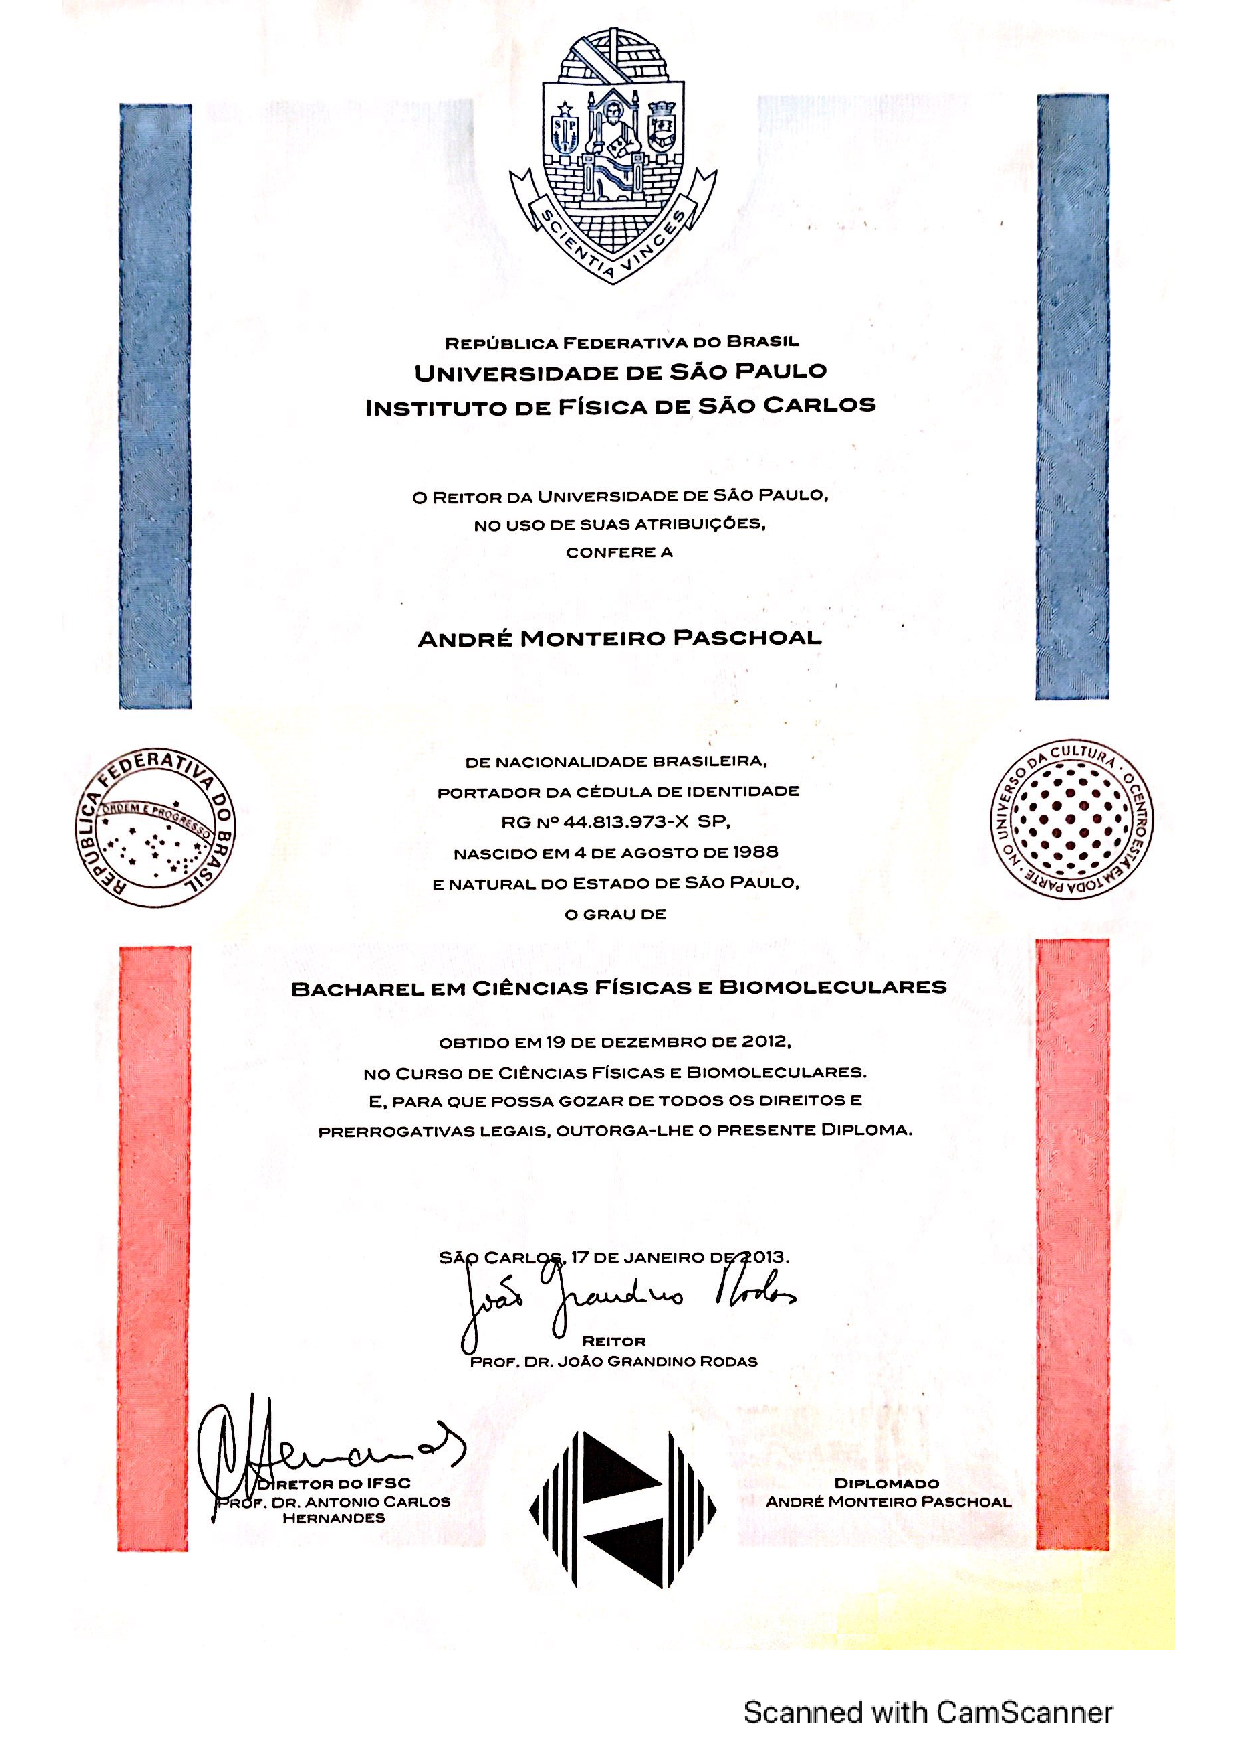
\includepdf[pages=-, scale=1,pagecommand=\thispagestyle{empty}]{\detokenize{Diplomas/DiplomaGraduaca}}

\newpage
\subsection{Atestado de estágio de iniciação científica no Laboratório de Química Medicinal e Computacional, localizado no 
Instituto de Física de São Carlos (IFSC - USP)}
\label{diplomas:IC}
Esta subseção apresenta o atestado de realização de iniciação científica no Laboratório de Química Medicinal e Computacional, localizado no 
Instituto de Física de São Carlos (IFSC - USP), desenvolvendo o projeto "Avaliação Biológica de Novos Agentes Anticâncer" sob orientação do Prof. 
Dr. Adriano D. Andricopulo no período de janeiro à dezembro de 2009.
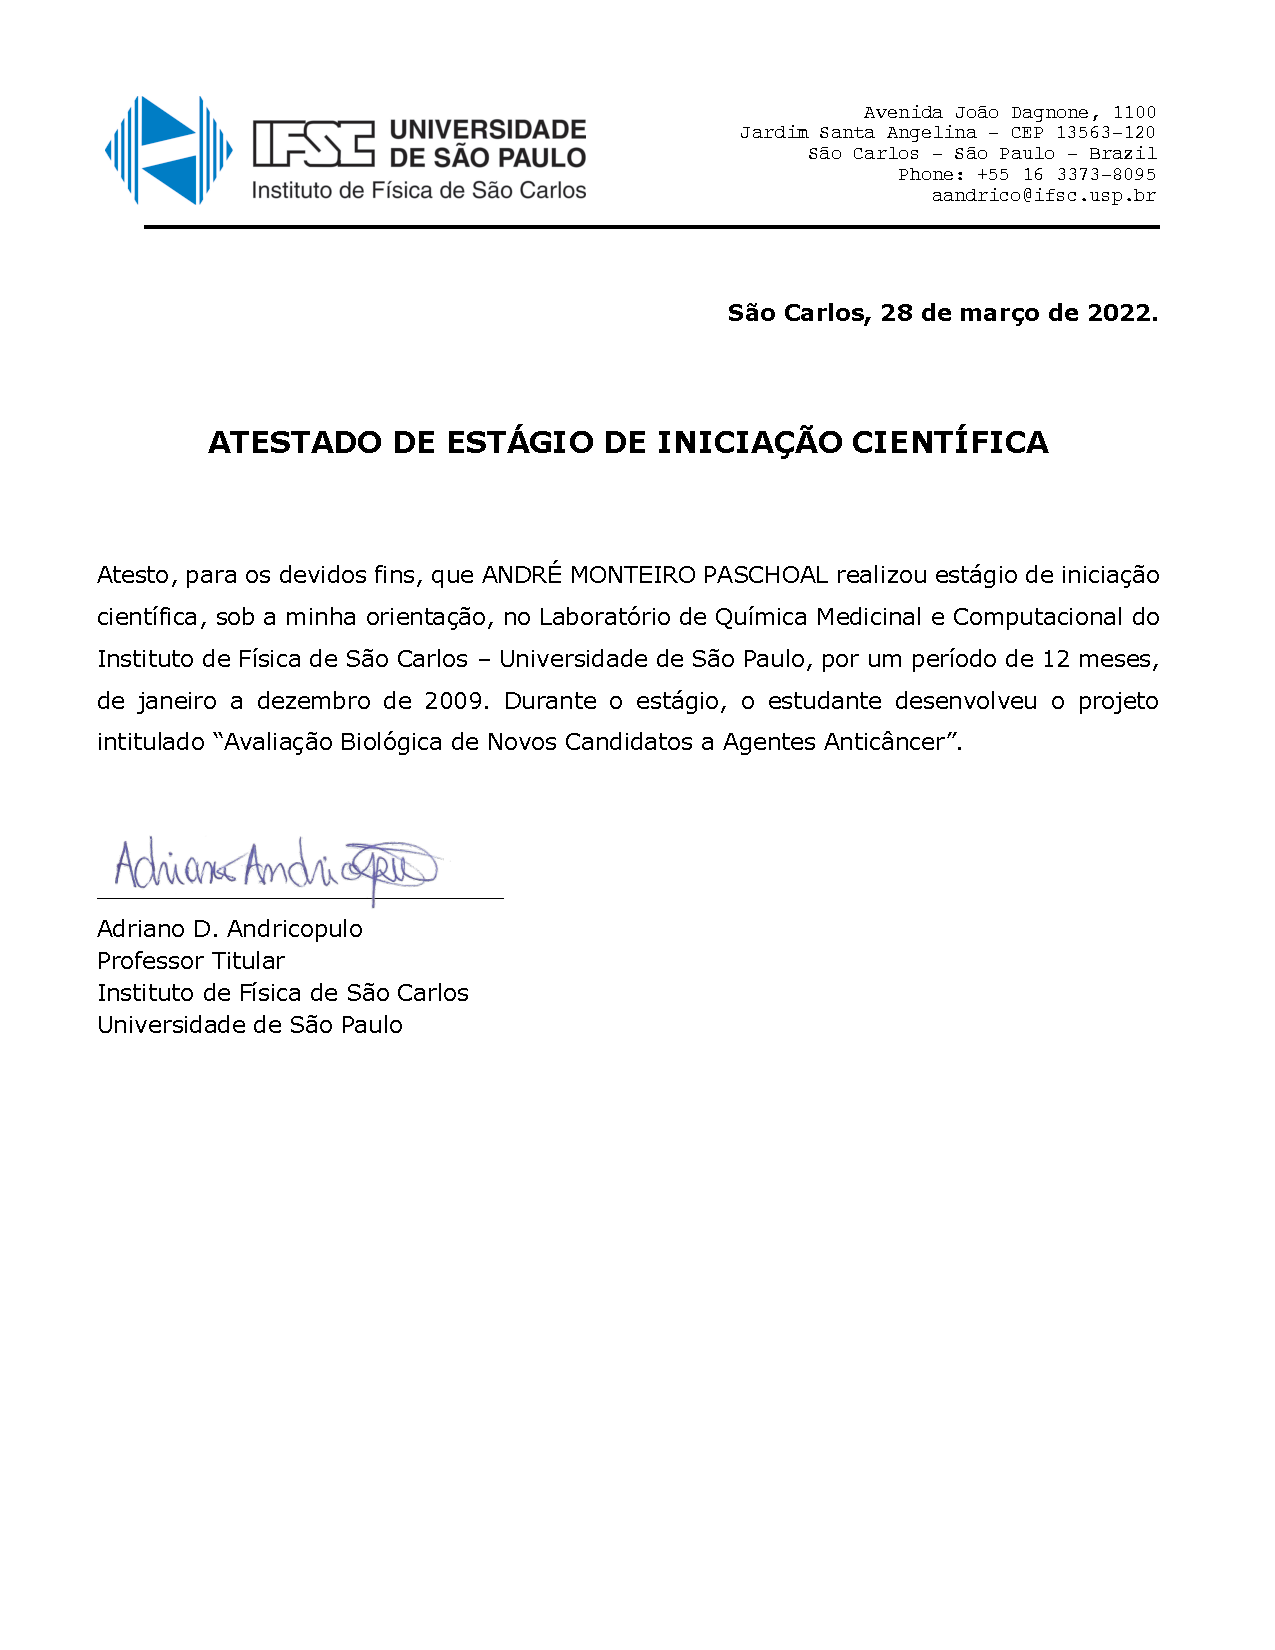
\includepdf[pages=-, scale=1,pagecommand=\thispagestyle{empty}]{\detokenize{Diplomas/IC_IFSC}}

\newpage
\subsection{Diploma de Mestre em Ciências, junto ao Instituto de Física de São Carlos (IFSC - USP)}
\label{diplomas:mestrado}
Esta subseção apresenta o diploma de Mestre em Ciências do candidato.
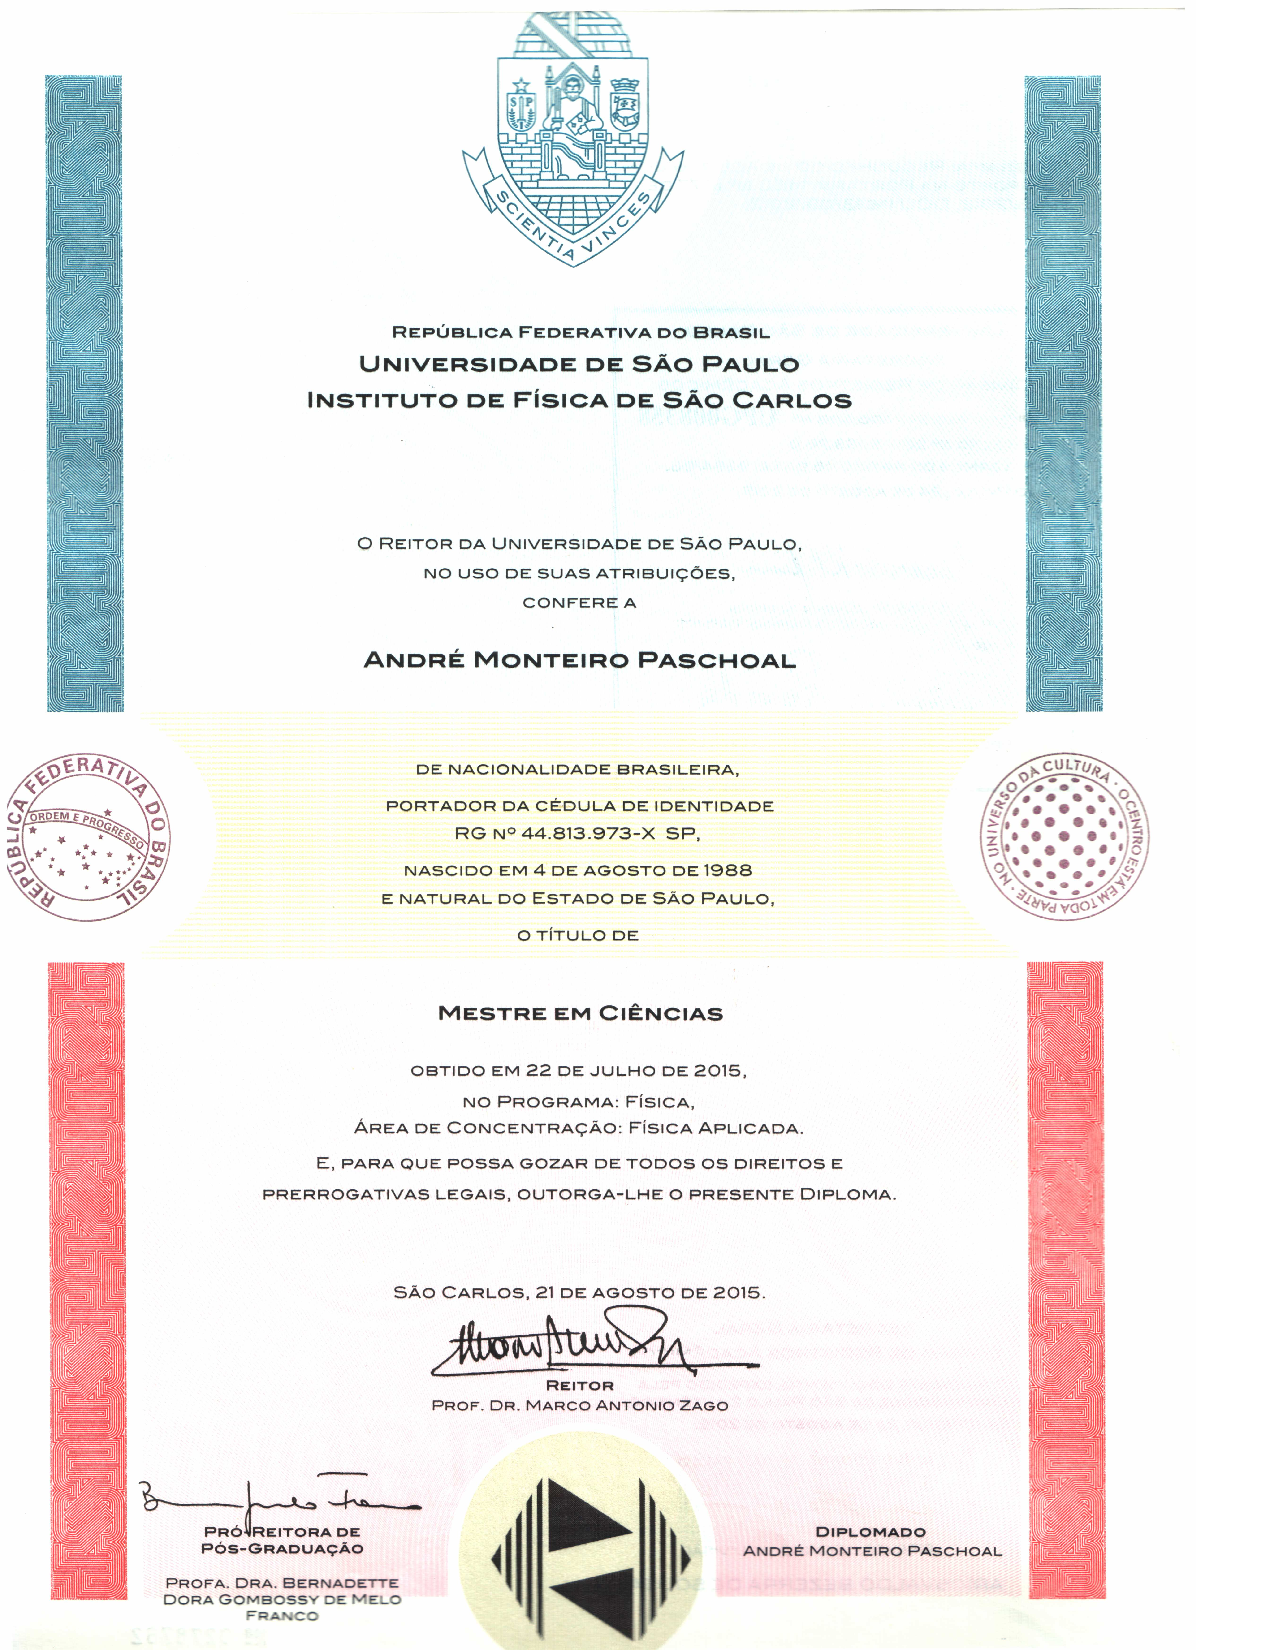
\includepdf[pages=-, scale=1,pagecommand=\thispagestyle{empty}]{\detokenize{Diplomas/diploma-mestrado}}

\newpage
\subsection{Diploma de Doutor em Ciências, junto ao Departamento de Física da Faculdade de Filosofia, Ciências e Letras de Ribeirão Preto (FFCLRP) da Universidade de São Paulo (USP)}
\label{diplomas:doutorado}
Esta subseção apresenta o diploma de Doutor em Ciências do candidato.
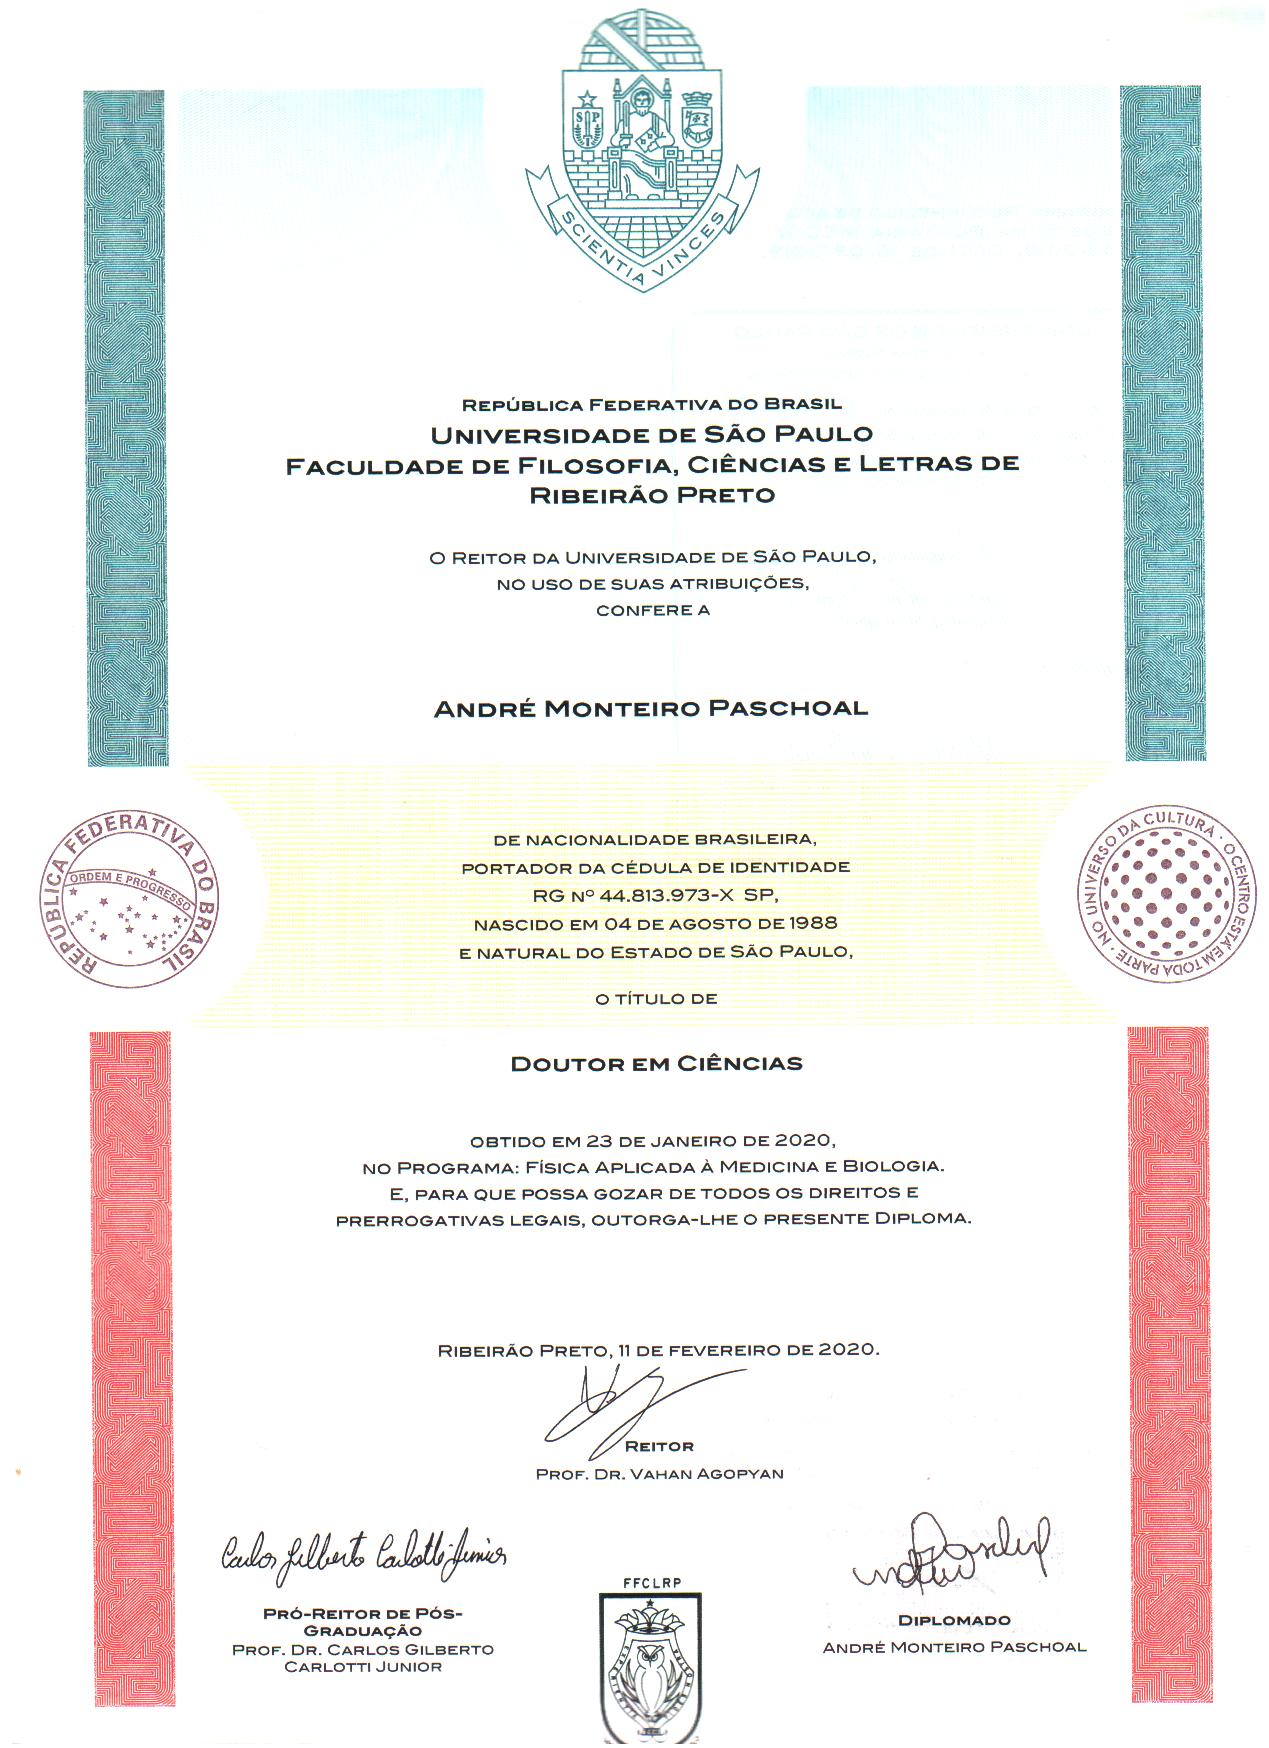
\includepdf[pages=-, scale=1,pagecommand=\thispagestyle{empty}]{\detokenize{Diplomas/PhDcertificate}}

\newpage
\subsection{Certificado de Pós Doutorado, junto à Faculdade de Medicina de Ribeirão Preto (FMRP) da Universidade de São Paulo (USP)}
\label{diplomas:posdoc1}
Esta subseção apresenta o certificado de conclusão do pós doutorado junto à FMRP do candidato.
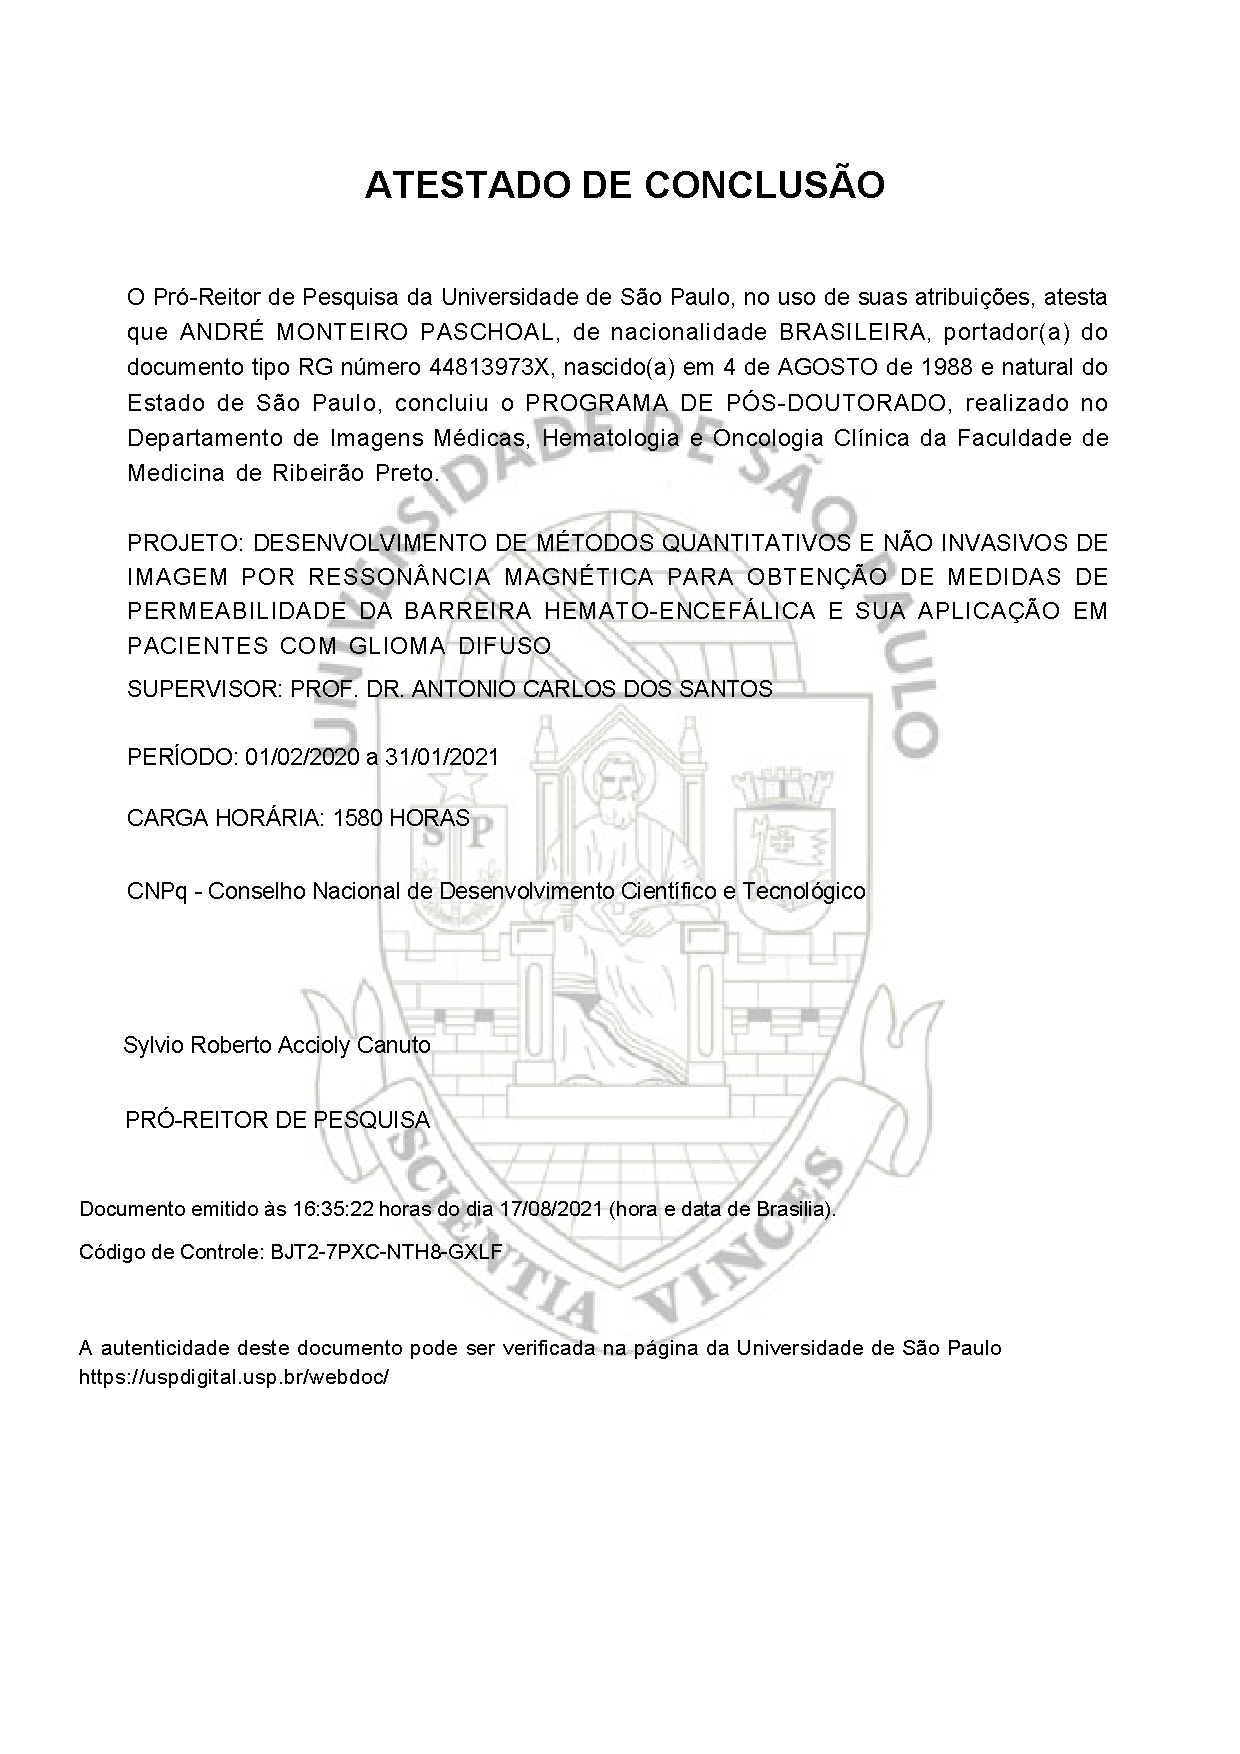
\includepdf[pages=-, scale=1,pagecommand=\thispagestyle{empty}]{\detokenize{Diplomas/posdocFMRP}}

\newpage
\subsection{Declaração de pesquisador, junto à Faculdade de Medicina da Universidade de São Paulo (FMUSP)}
\label{diplomas:posdoc2}
Esta subseção apresenta a declaração das atividades do candidato como pesquisador no Instituto de Radiologia, da Faculdade de Medicina da Universidade de São 
Paulo.
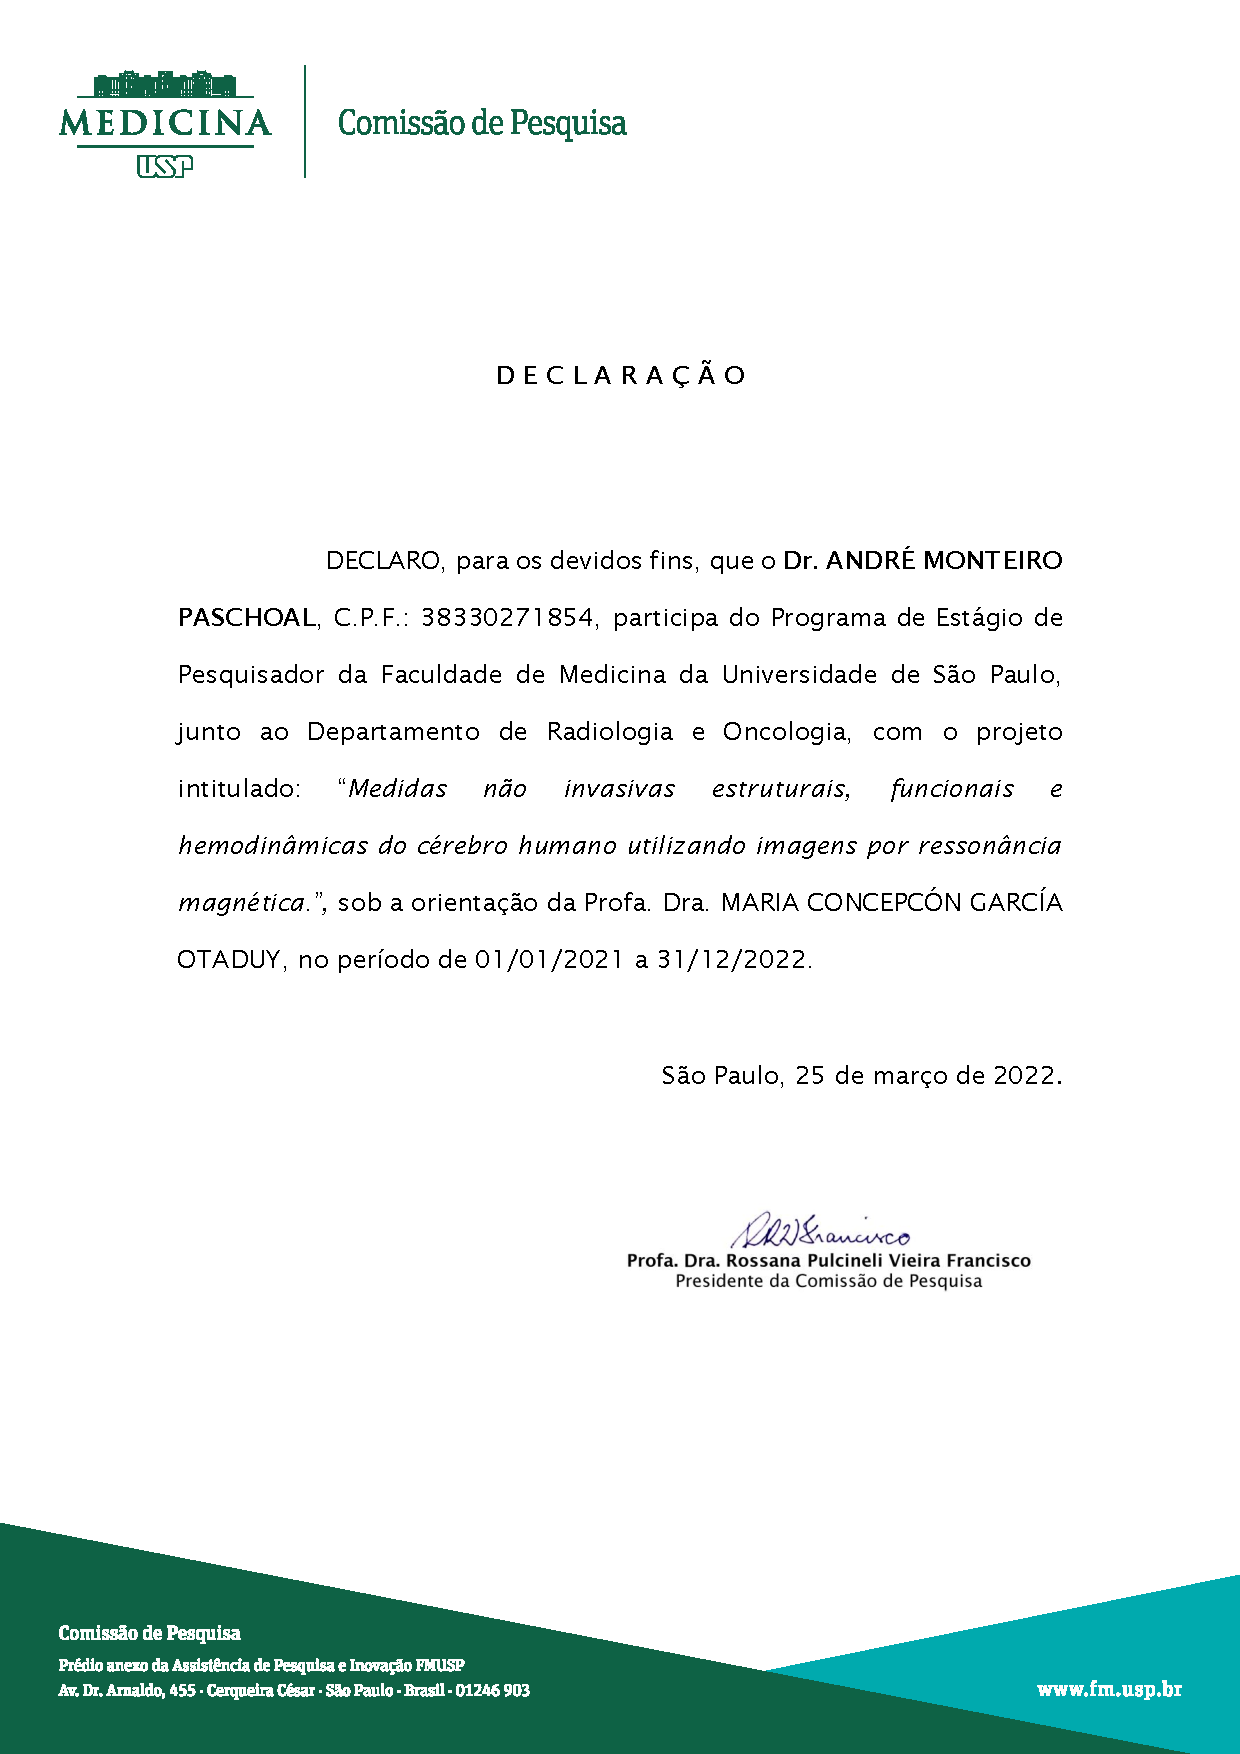
\includepdf[pages=-, scale=1,pagecommand=\thispagestyle{empty}]{\detokenize{Diplomas/declaracaoEstagioInRad}}

\newpage
\subsection{Participação como pesquisador associado no projeto FAPESP número 2019/06148-6}
\label{certificados:fapesp_regular2019}
Esta subseção apresenta o comprovante de participação como pesquisador associado no projeto FAPESP número 2019/06148-6.
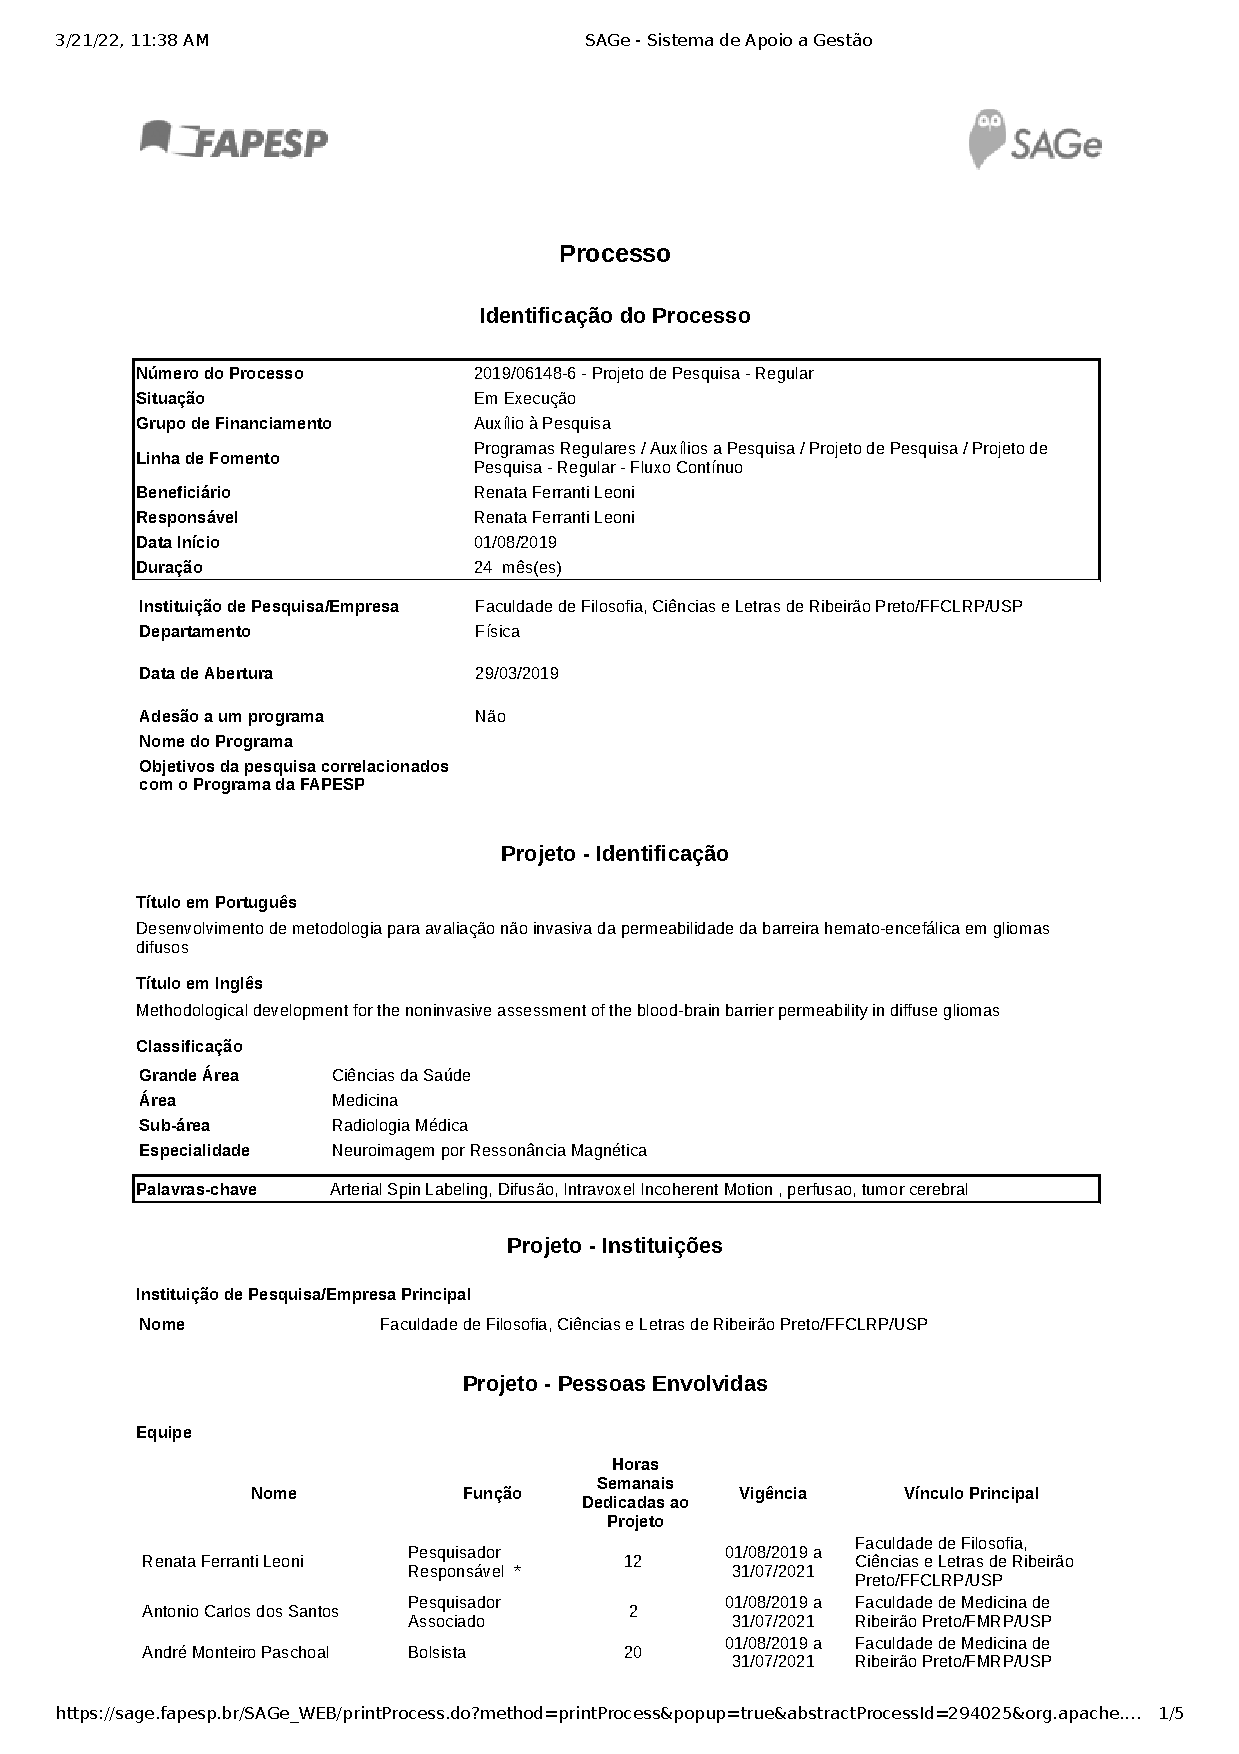
\includepdf[pages=-, scale=1,pagecommand=\thispagestyle{empty}]{\detokenize{Diplomas/fapesp_renata2019}}

\newpage
\subsection{Declaração de realização de estágio remunerado}
\label{declaracao:SAPRA}
Esta subseção apresenta a declaração de realização de estágio remunerado na empresa SAPRA-Landauer Serviço de Assessoria e Proteção Radiológica Ltda no período 
de 08 de fevereiro à 07 de dezembro de 2012.
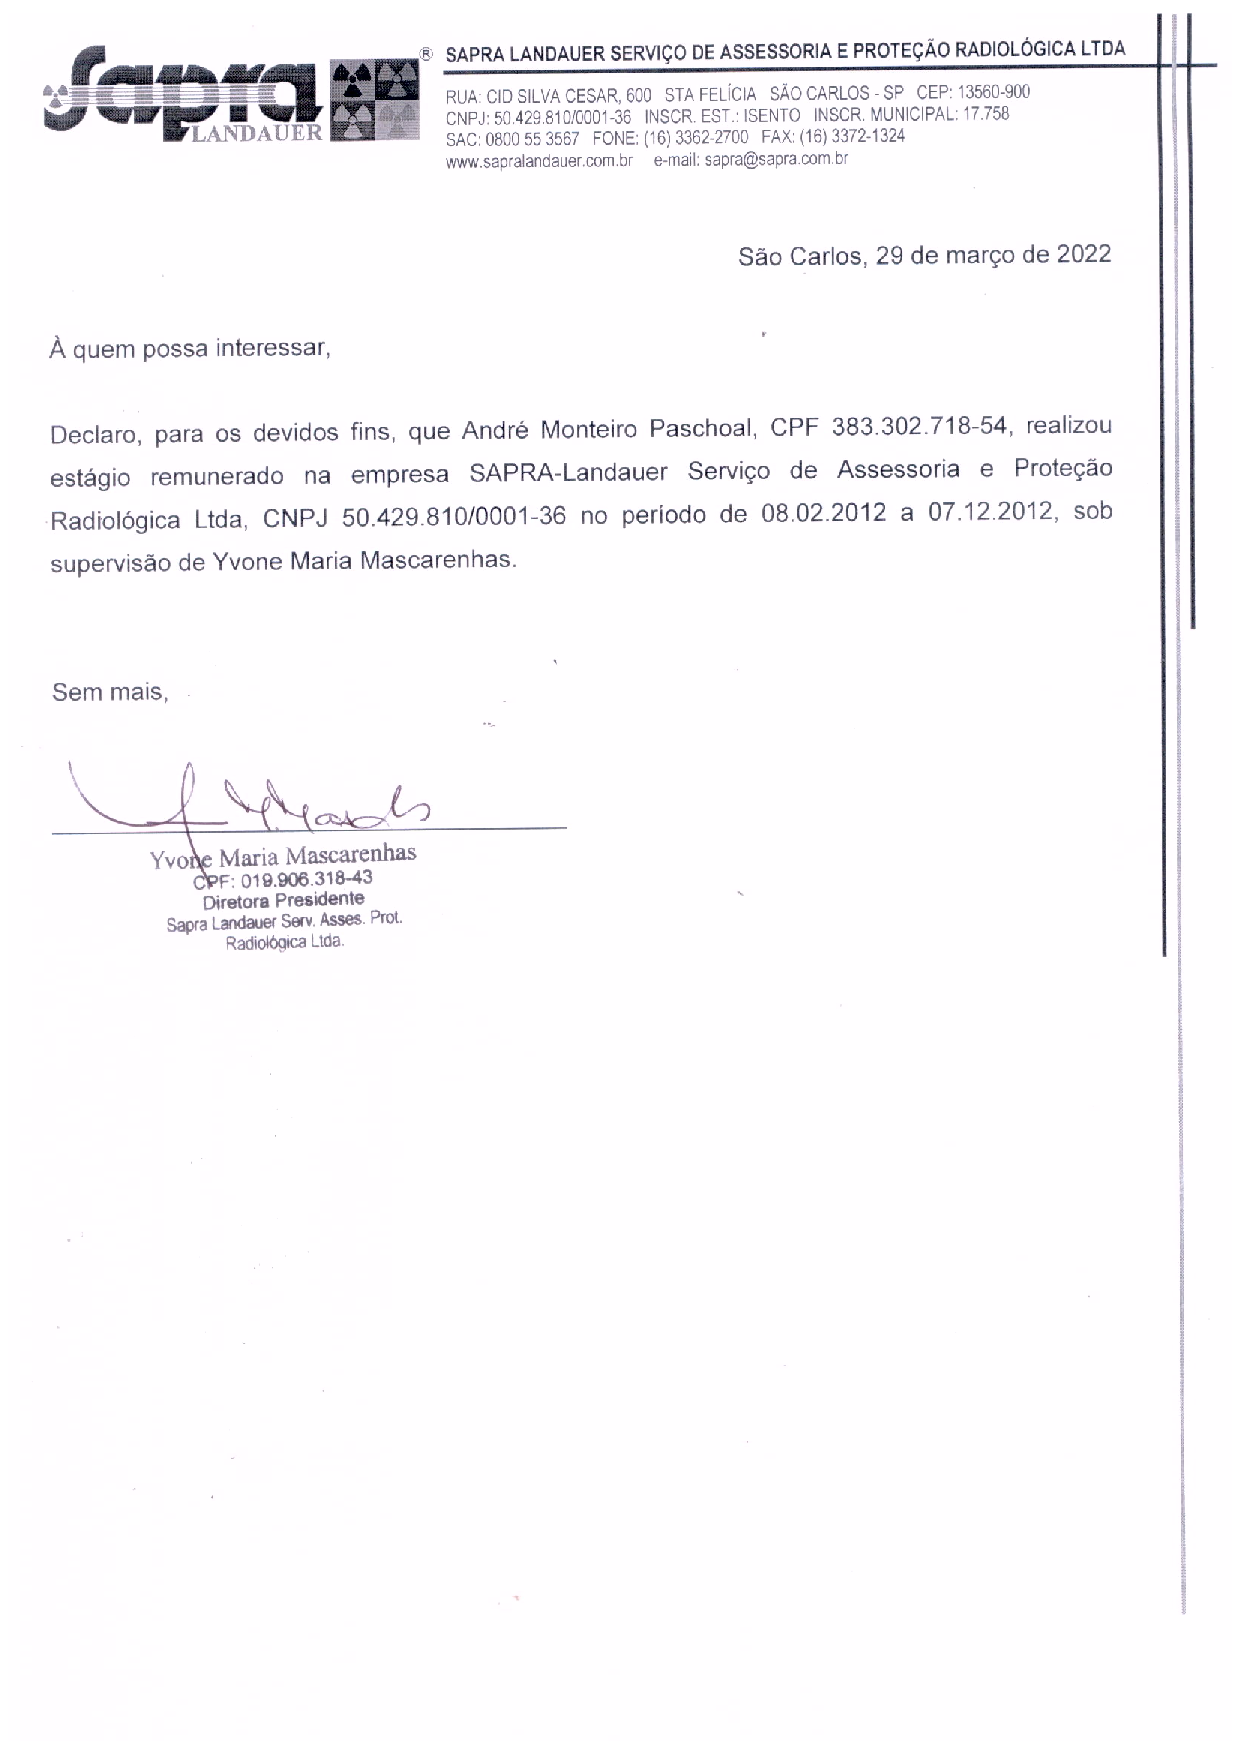
\includepdf[pages=-, scale=1,pagecommand=\thispagestyle{empty}]{\detokenize{Diplomas/estagioSAPRA}}

\newpage
\subsection{Certificado de conclusão do MRI Graduate Program pela Universidade de Oxford}
\label{diplomas:oxford}
Esta subseção apresenta o comprovante de conclusão do curso MRI \textit{Graduate Program}, oferecido pelo programa WIN da Universidade de Oxford, 
com duração de um ano.

\includepdf[pages=-, scale=1,pagecommand=\thispagestyle{empty}]{\detokenize{Diplomas/MRIoxford}}

\newpage
\subsection{Prêmios de mérito científico}
\label{awards:OHBM}
Esta subseção apresenta o certificado de obtenção do Prêmio \textbf{OHBM Travel Award}, concedido no Encontro Anual da \textit{Organization for Human Brain Mapping} no ano de 2019, realizado em Roma - Itália.
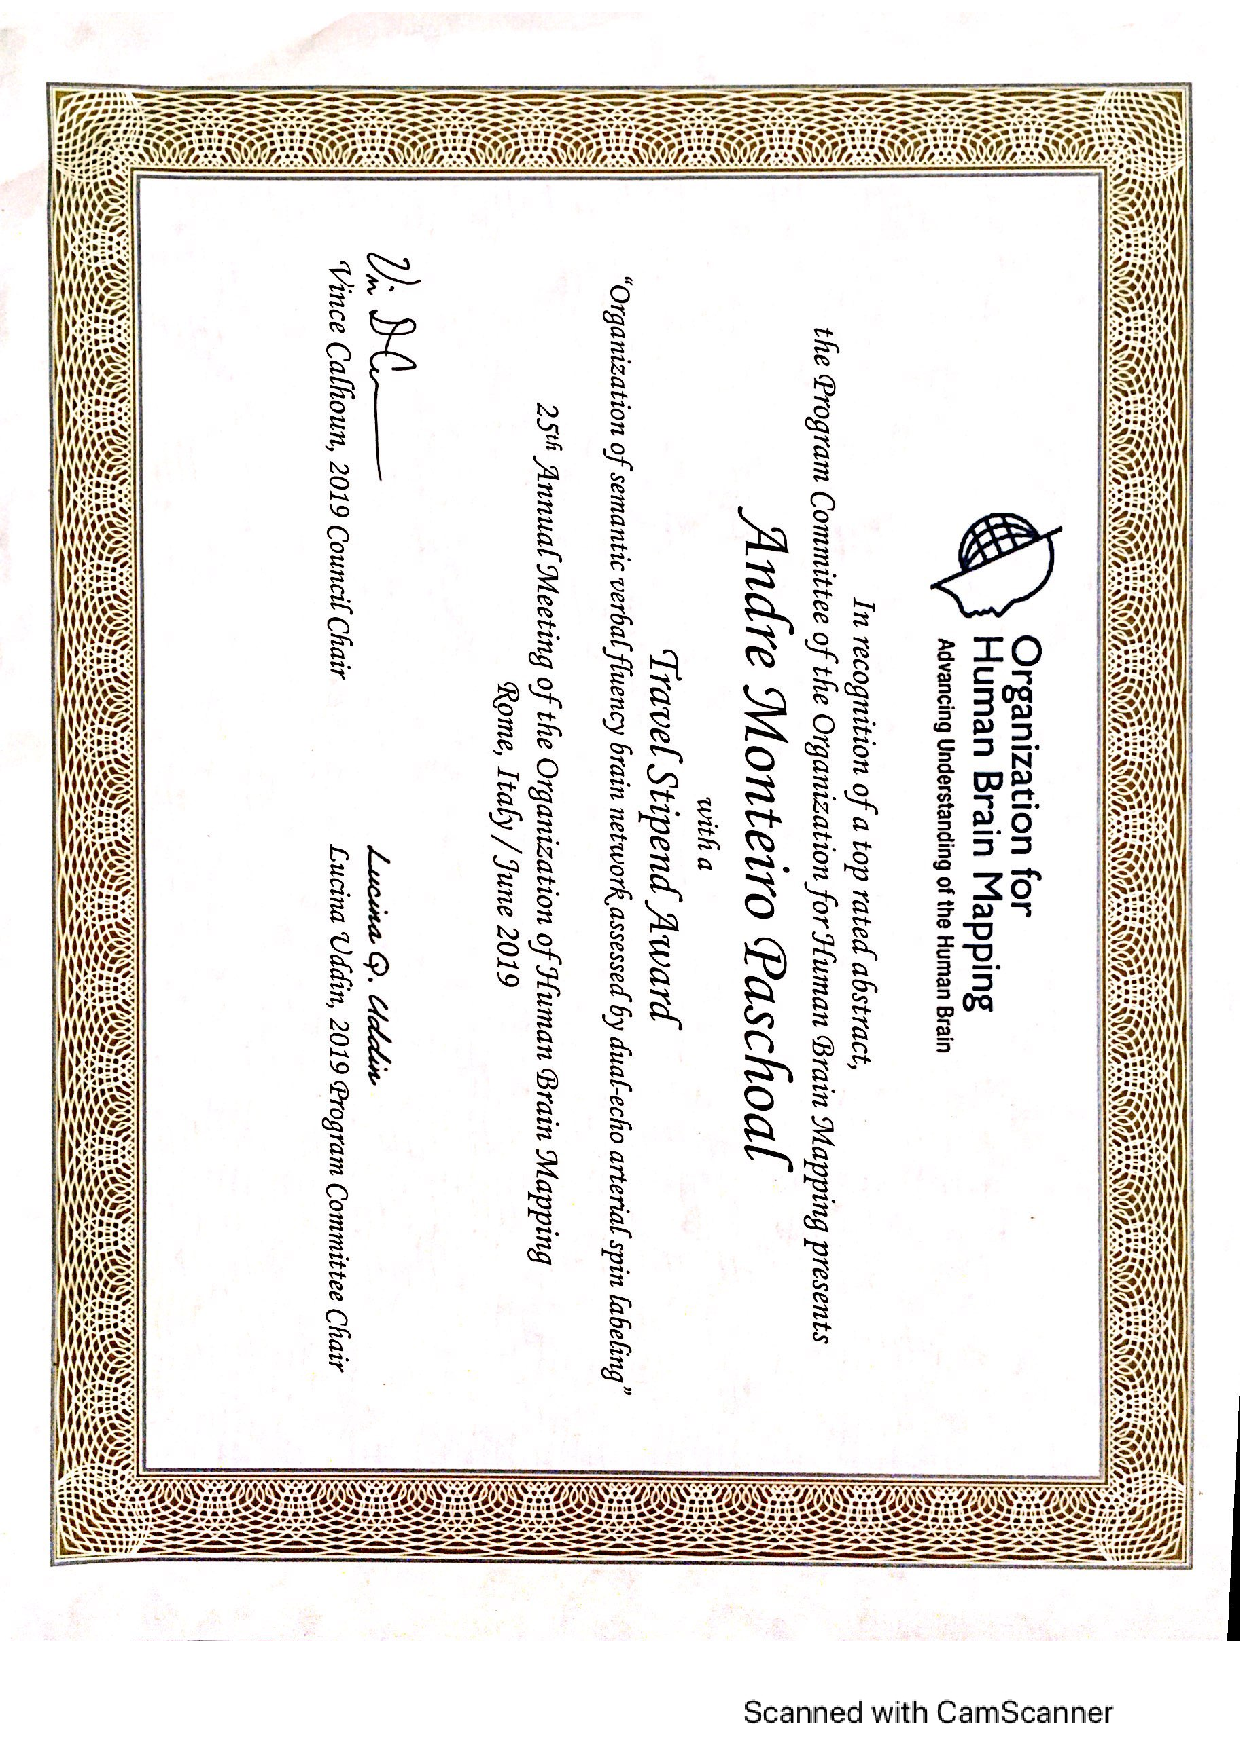
\includepdf[pages=-, scale=1,pagecommand=\thispagestyle{empty}]{\detokenize{Diplomas/OHBMtravelAward}}

\newpage
\subsection{Prêmios de mérito científico - Prêmio CAPES de Teses}
\label{awards:CAPES}
Esta subseção apresenta o certificado de obtenção da Menção Honrosa no \textbf{Prêmio CAPES de Teses 2021}, concedido pela CAPES no ano de 2021.
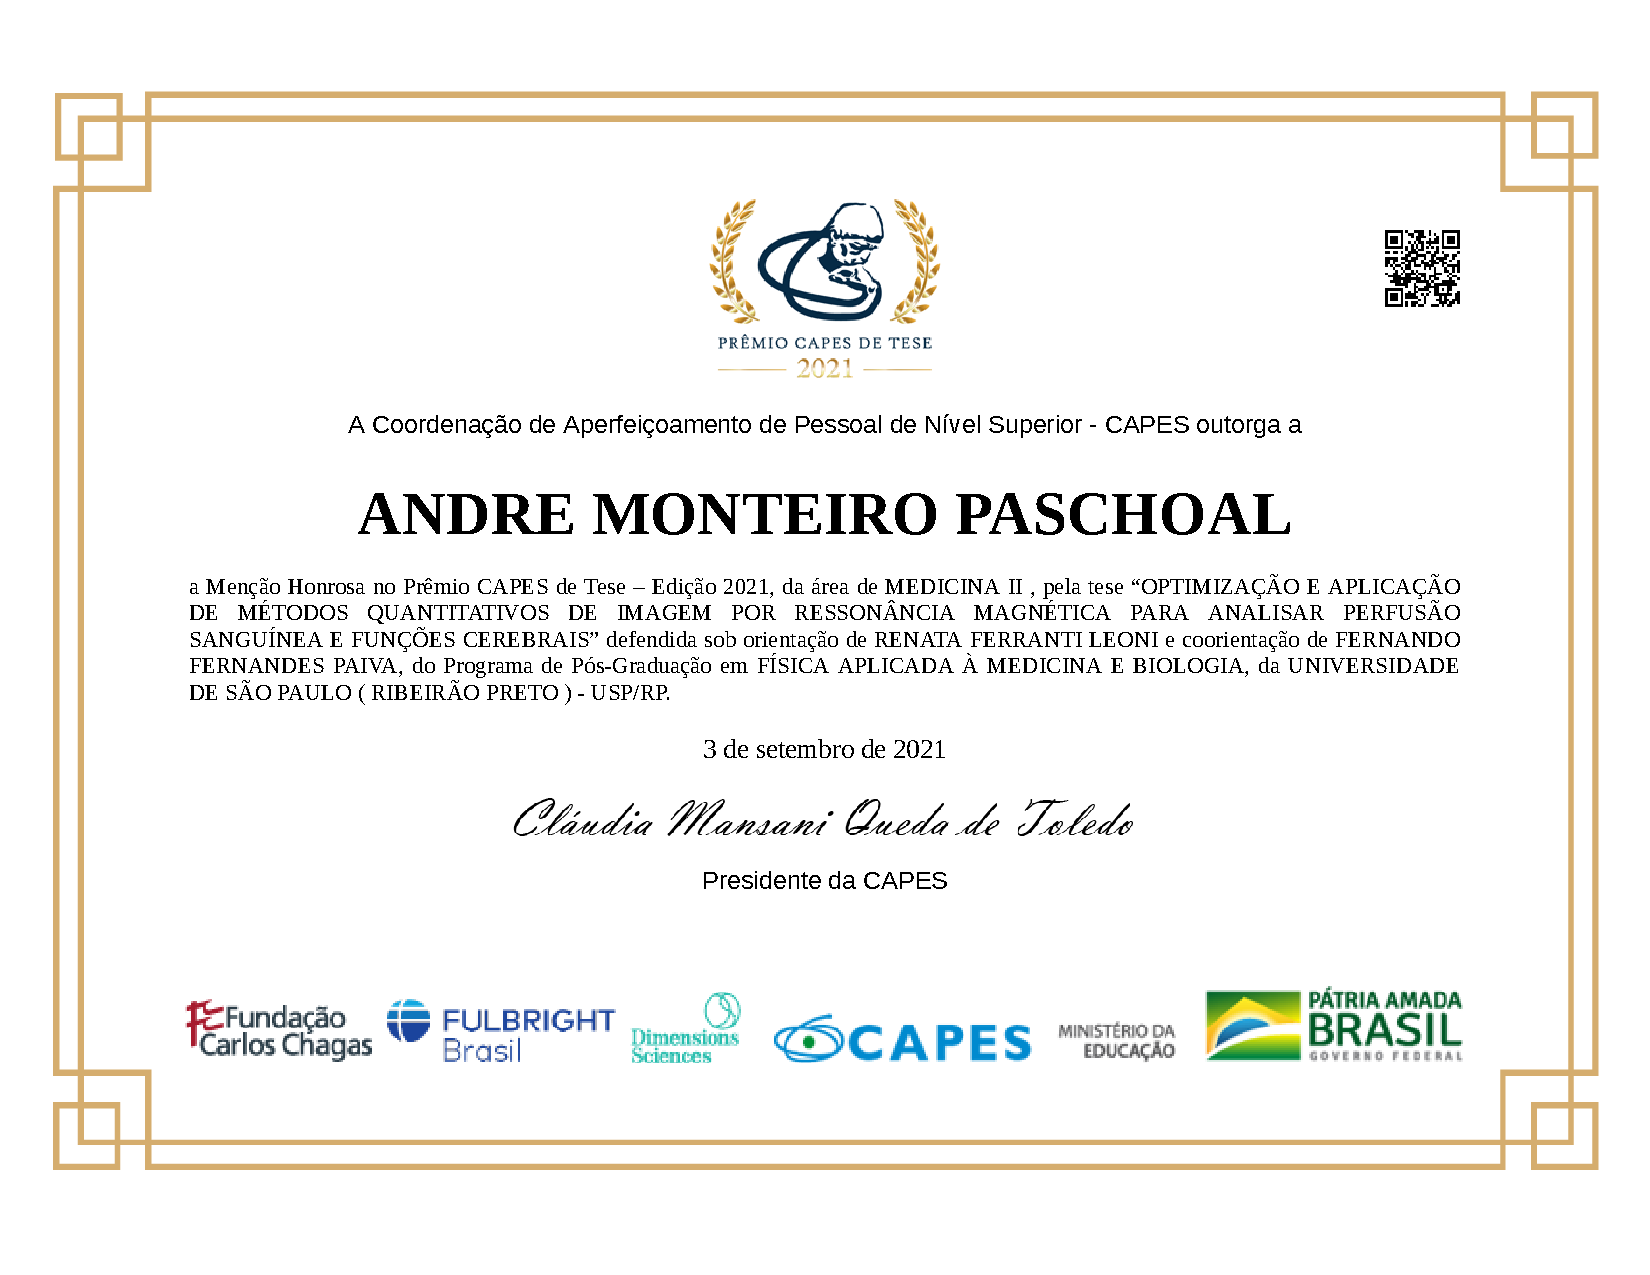
\includepdf[pages=-, scale=1,pagecommand=\thispagestyle{empty}]{\detokenize{Diplomas/premioCAPES}}

%%%%%%%%%%%%%%%%%%%%%%%%%%%%%%%%%%%%%%%%%%%%%%%%%%%%%%%%%%%%%%%%%%%%%%%%%%%%%%%
% Subgrupo 2.1 - Produtividade de Pesquisa
%%%%%%%%%%%%%%%%%%%%%%%%%%%%%%%%%%%%%%%%%%%%%%%%%%%%%%%%%%%%%%%%%%%%%%%%%%%%%%%

\newpage
\subsection{Participa\c{c}\~{a}o em Eventos Cient\'{\i}ficos (com apresenta\c{c}\~{a}o de trabalho ou oferecimento de cursos, palestras ou debates}
\label{certificados:SIFSC2013}
Esta subseção apresenta o comprovante da participação na III Semana Integrada do Instituto de Física de São Carlos com seus respectivos propósitos.
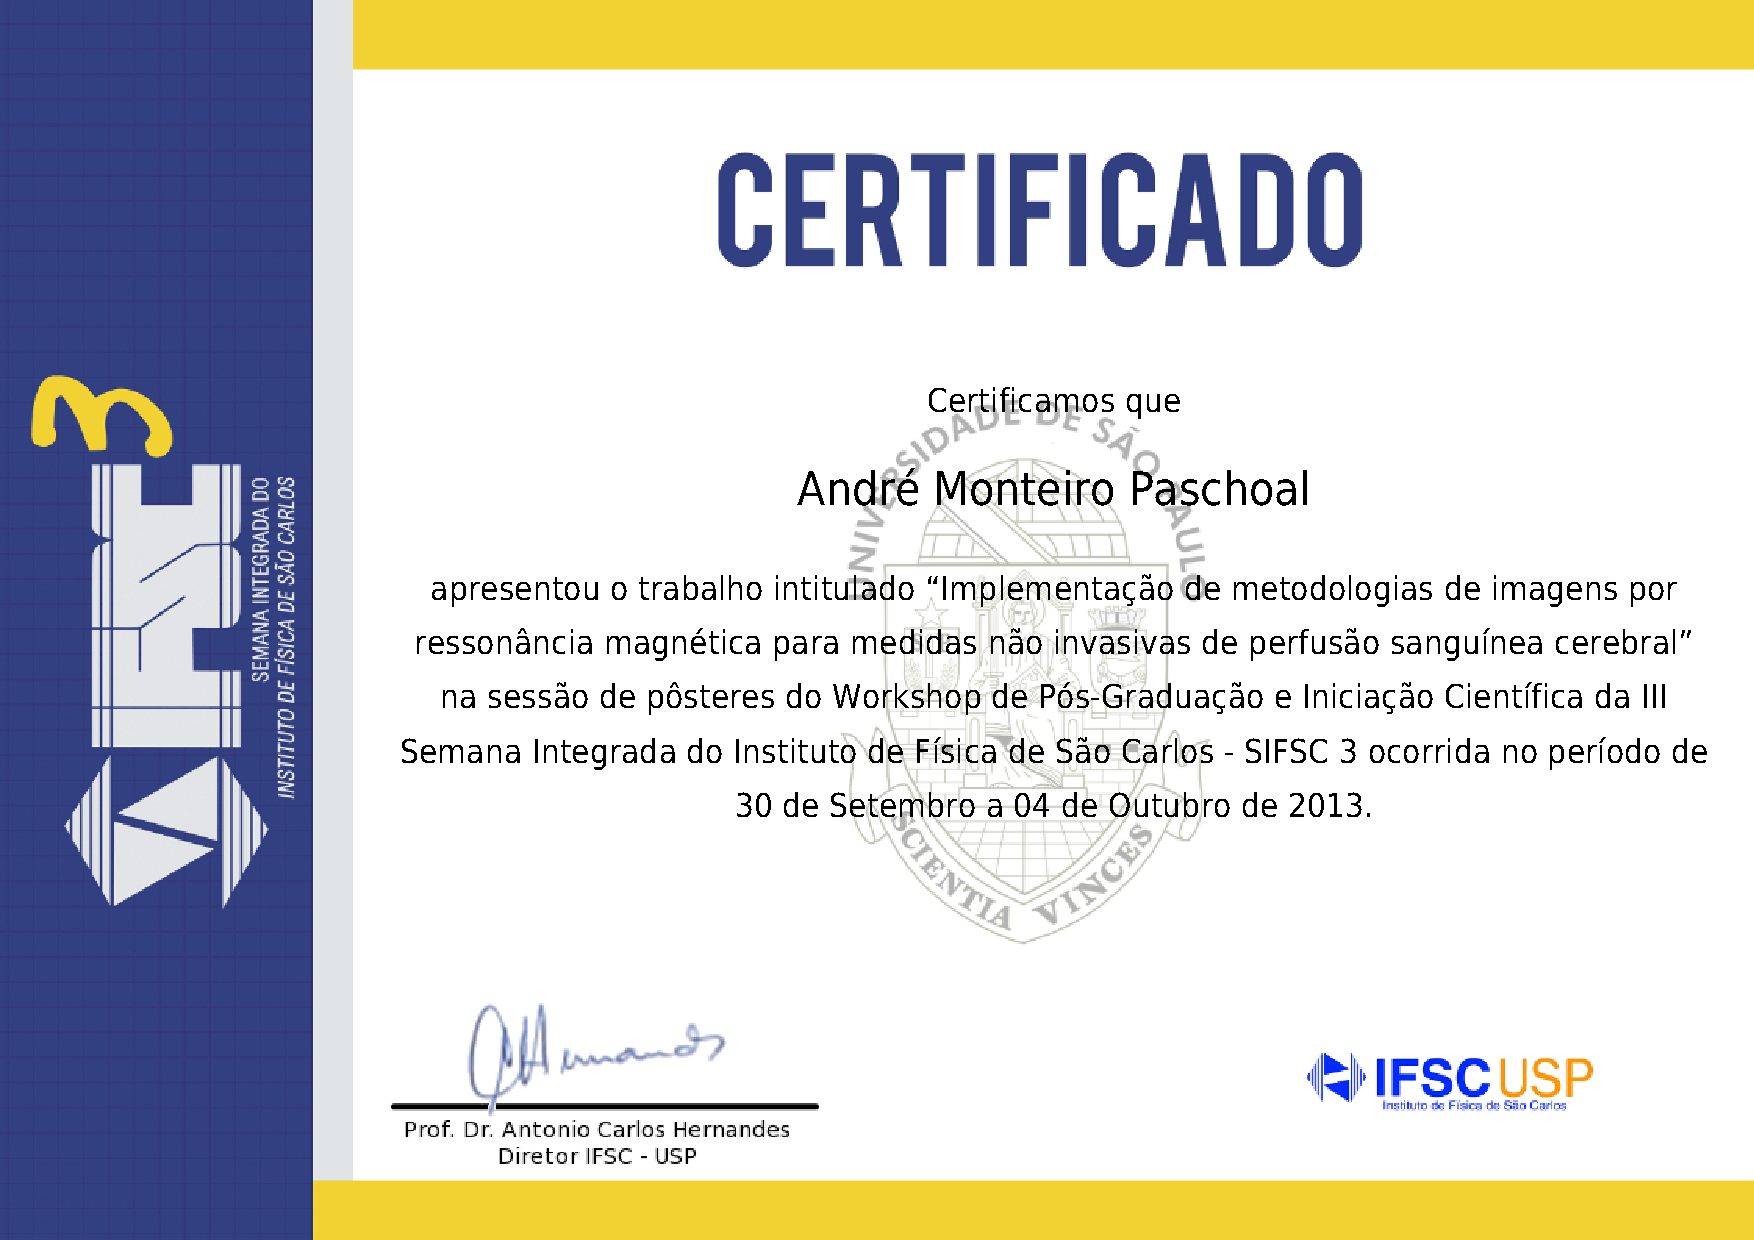
\includepdf[pages=-, scale=1,pagecommand=\thispagestyle{empty}]{\detokenize{Diplomas/CertificadoSIFSC2013}}

\newpage
\subsection{Participa\c{c}\~{a}o em Eventos Cient\'{\i}ficos (com apresenta\c{c}\~{a}o de trabalho ou oferecimento de cursos, palestras ou debates}
\label{certificados:SIFSC2014}
Esta subseção apresenta o comprovante da participação na IV Semana Integrada do Instituto de Física de São Carlos com seus respectivos propósitos.
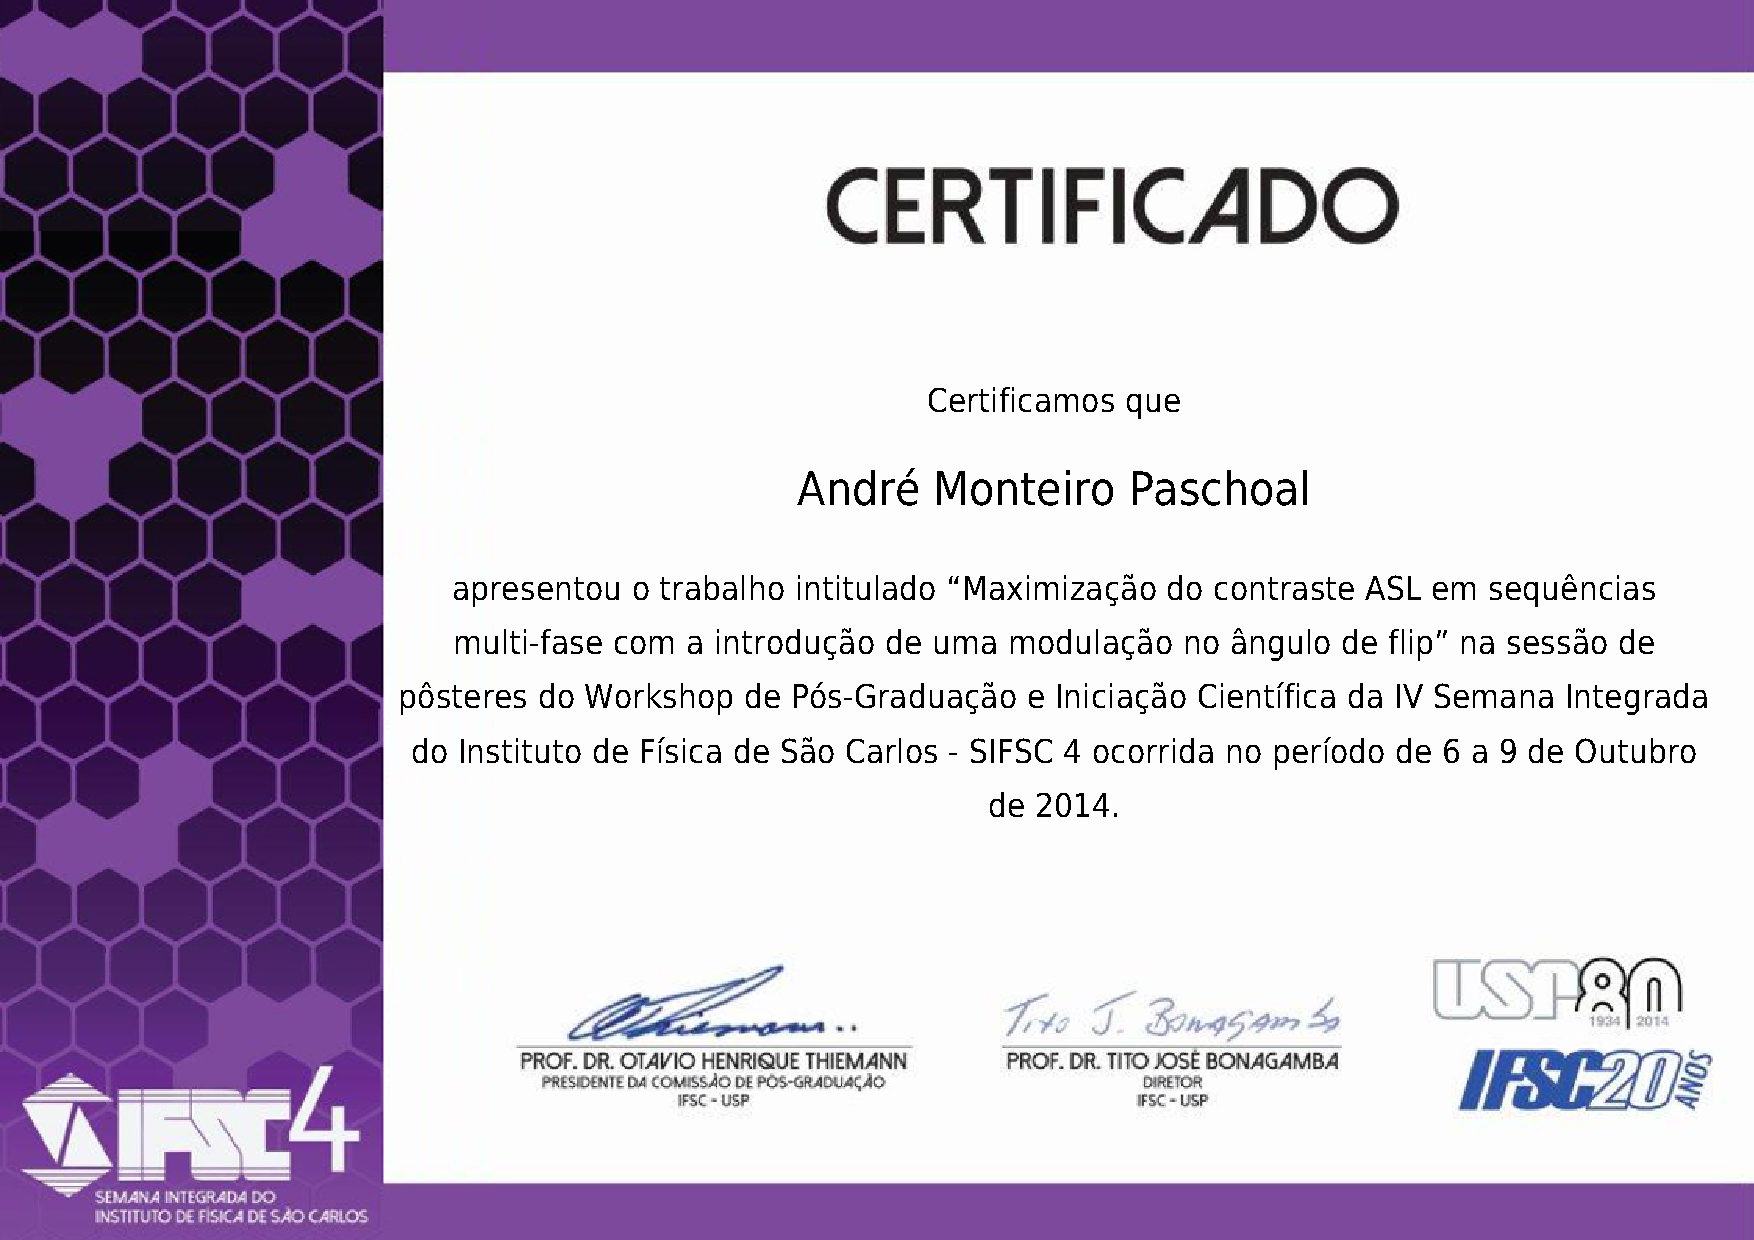
\includepdf[pages=-, scale=1,pagecommand=\thispagestyle{empty}]{\detokenize{Diplomas/CertificadoSIFSC2014}}

\newpage
\subsection{Participa\c{c}\~{a}o em Eventos Cient\'{\i}ficos (com apresenta\c{c}\~{a}o de trabalho ou oferecimento de cursos, palestras ou debates}
\label{certificados:Transatlantic}
Esta subseção apresenta o comprovante da participação no I Transatlantic Workshop on Methods for Multimodal Neurosciences Studies com seus respectivos propósitos.
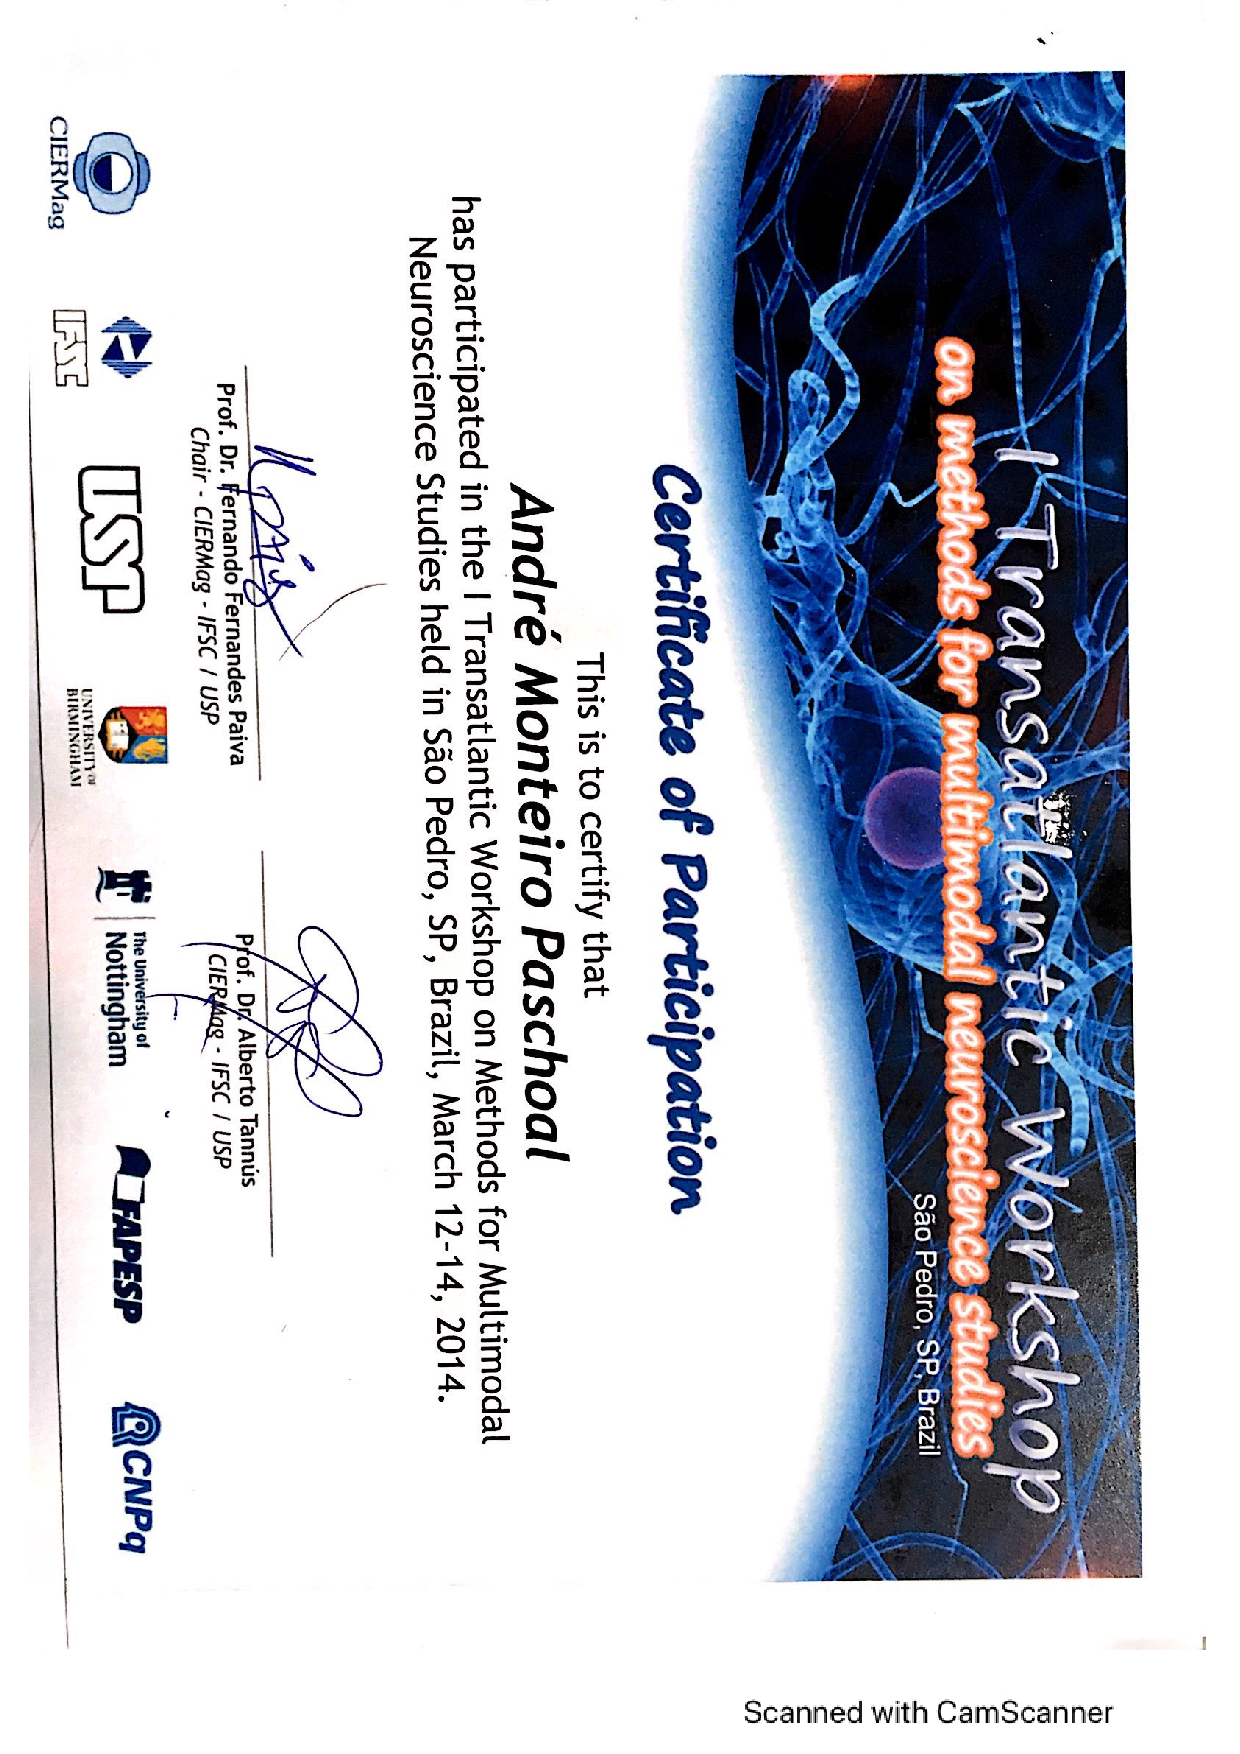
\includepdf[pages=-, scale=1,pagecommand=\thispagestyle{empty}]{\detokenize{Diplomas/TransatlanticWorkshopParticipation}}
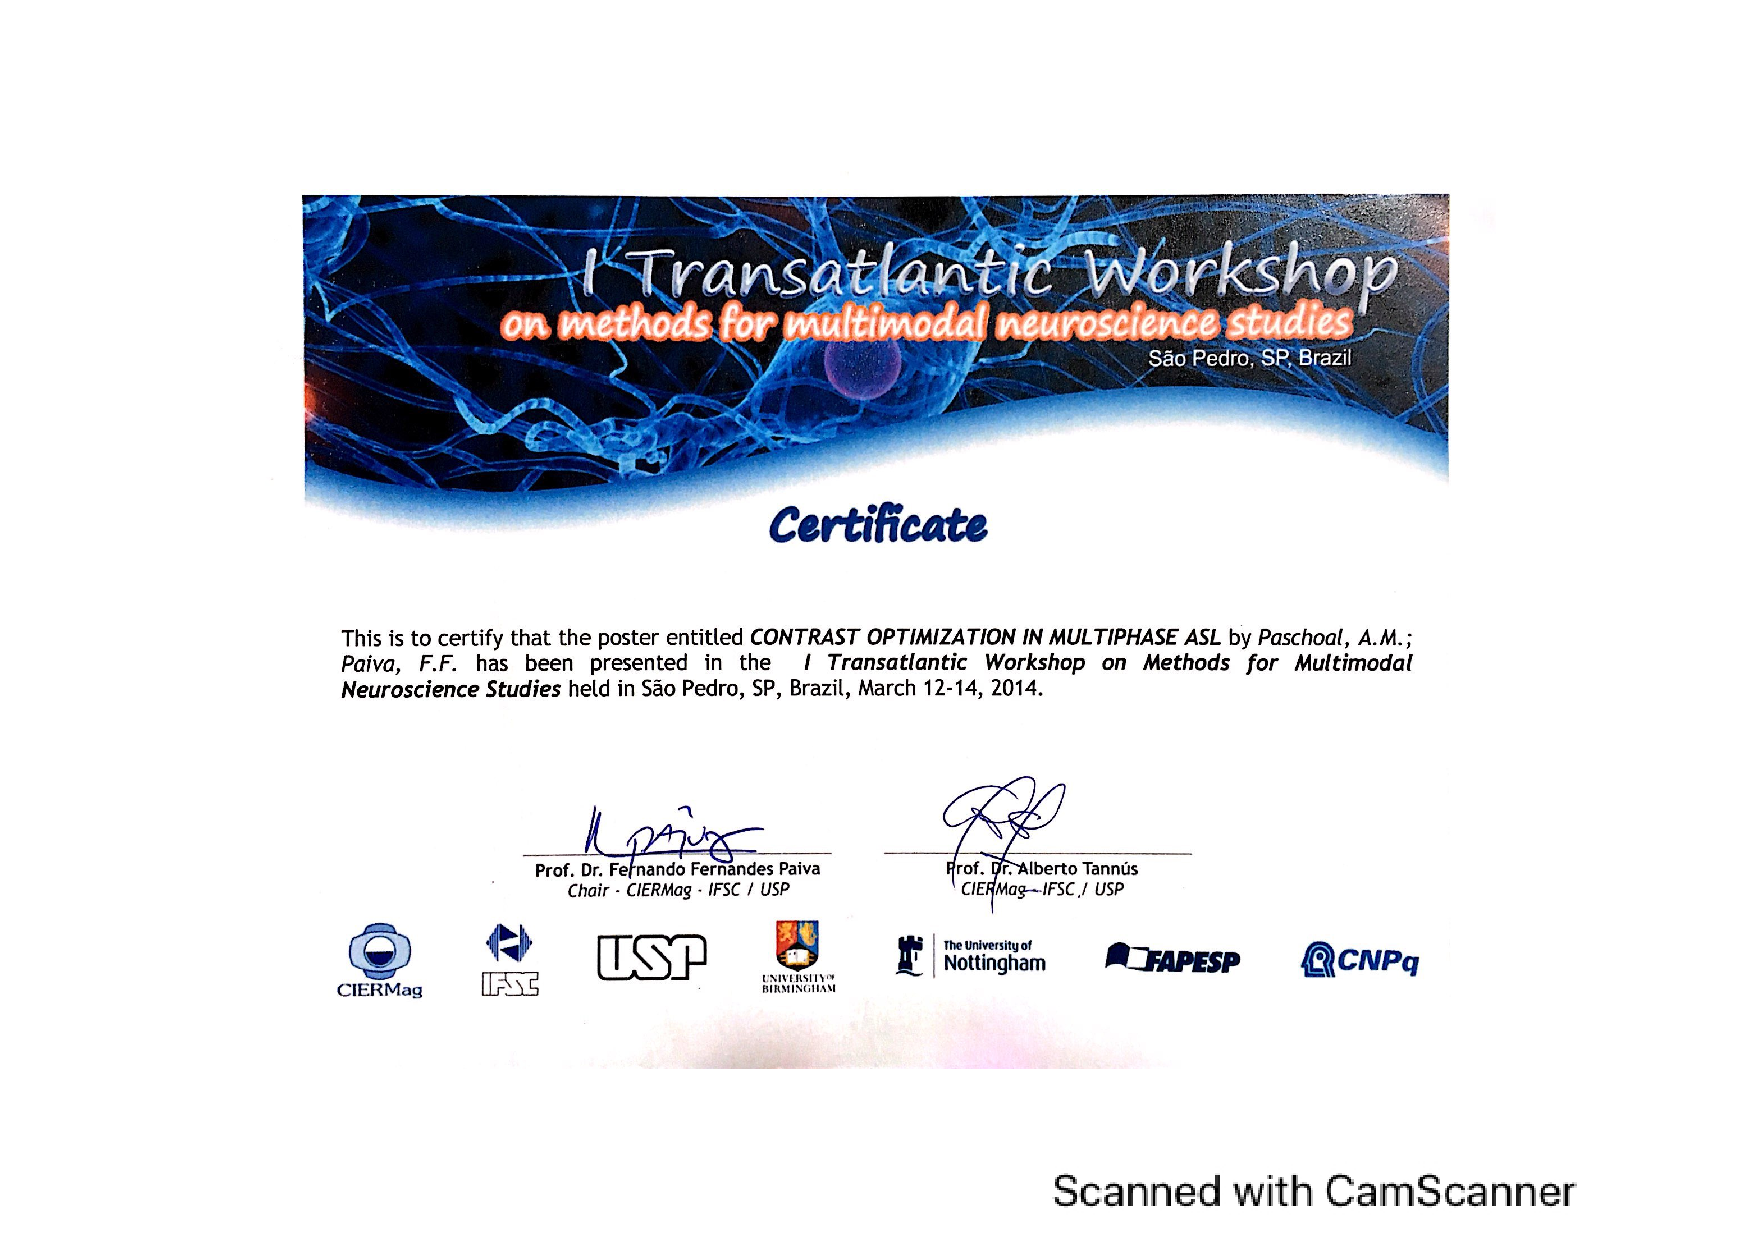
\includepdf[pages=-, scale=1,pagecommand=\thispagestyle{empty}]{\detokenize{Diplomas/TransatlanticWorkshopPresentation}}

\newpage
\subsection{Participa\c{c}\~{a}o em Eventos Cient\'{\i}ficos (com apresenta\c{c}\~{a}o de trabalho ou oferecimento de cursos, palestras ou debates}
\label{certificados:SIFSC2015}
Esta subseção apresenta o comprovante da participação na V Semana Integrada do Instituto de Física de São Carlos com seus respectivos propósitos.
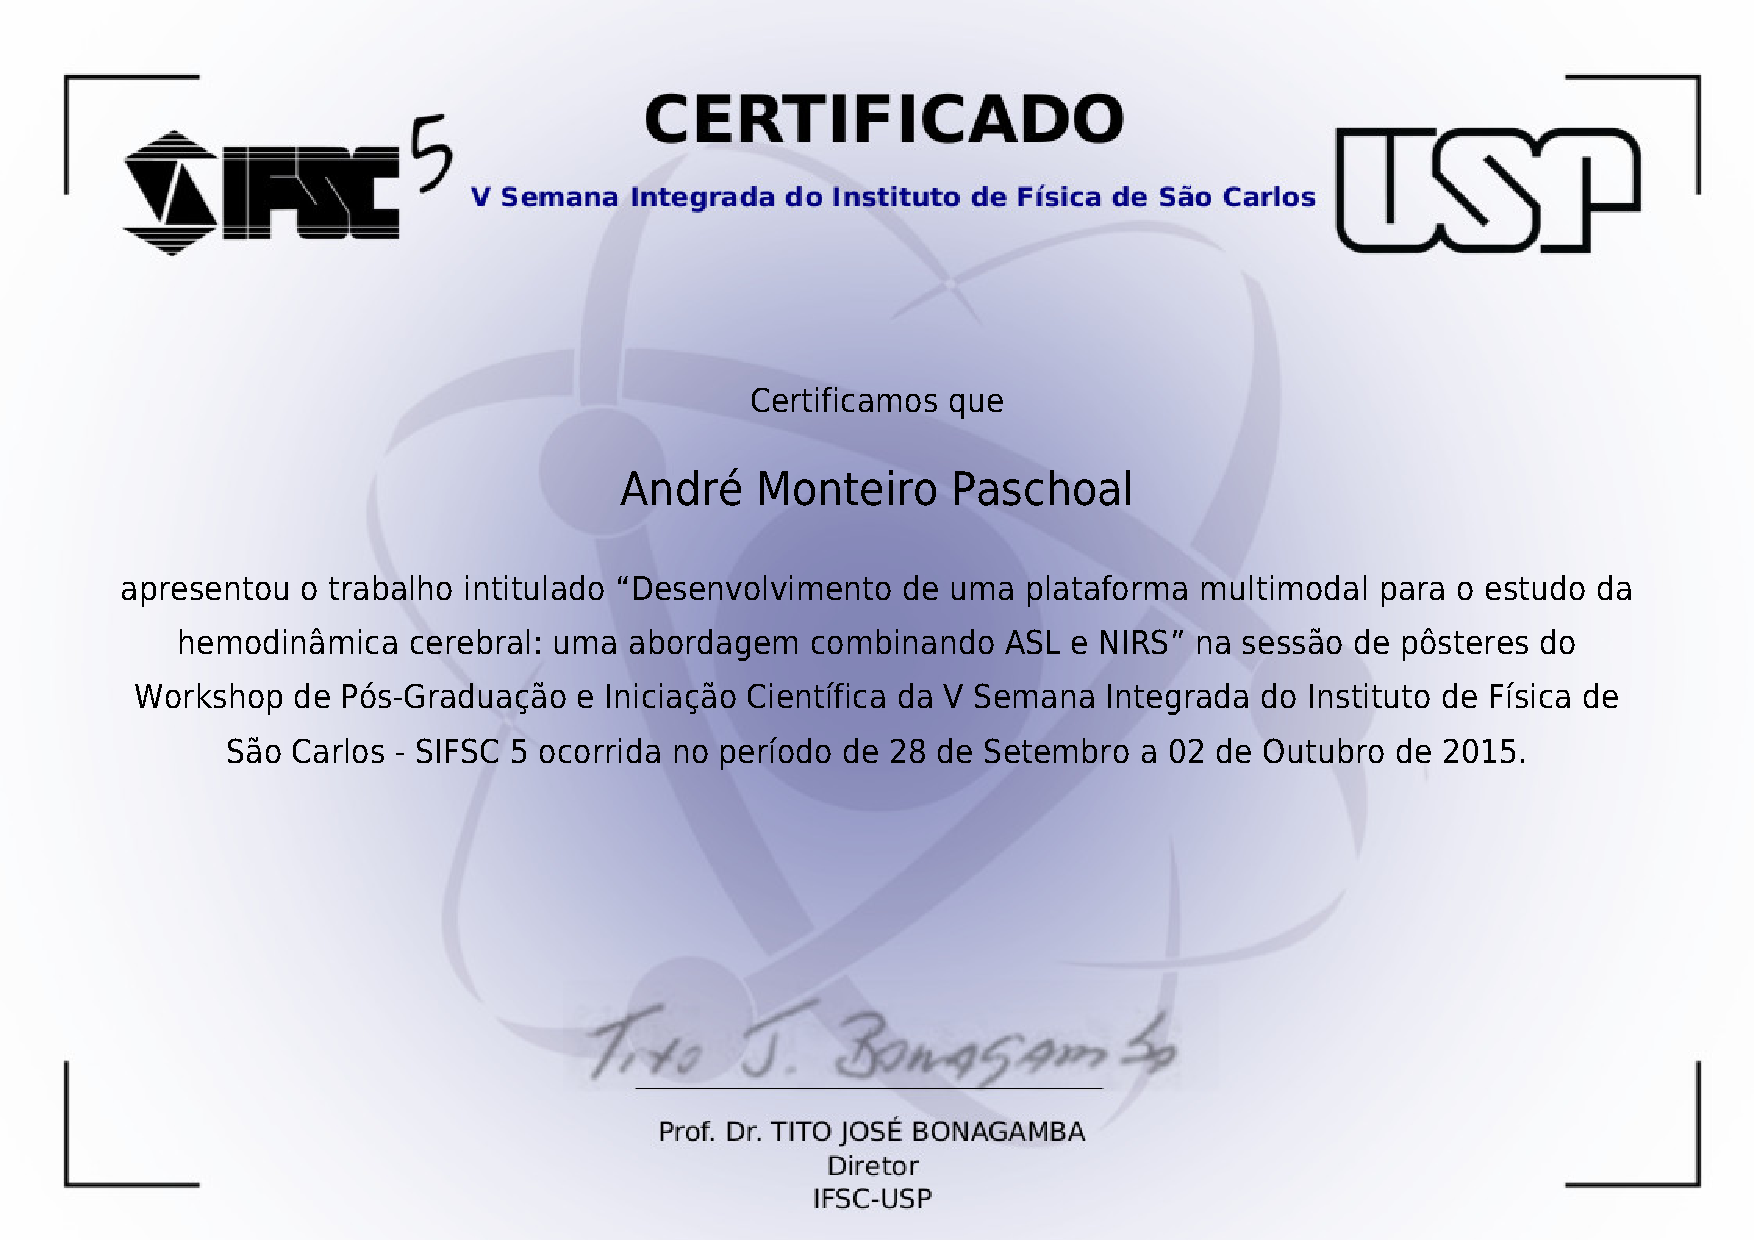
\includepdf[pages=-, scale=1,pagecommand=\thispagestyle{empty}]{\detokenize{Diplomas/CertificadoSIFSC2015}}

\newpage
\subsection{Participa\c{c}\~{a}o em Eventos Cient\'{\i}ficos (com apresenta\c{c}\~{a}o de trabalho ou oferecimento de cursos, palestras ou debates}
\label{certificados:SFM2016}
Esta subseção apresenta o comprovante da participação na XV Semana da Física Médica com seus respectivos propósitos.
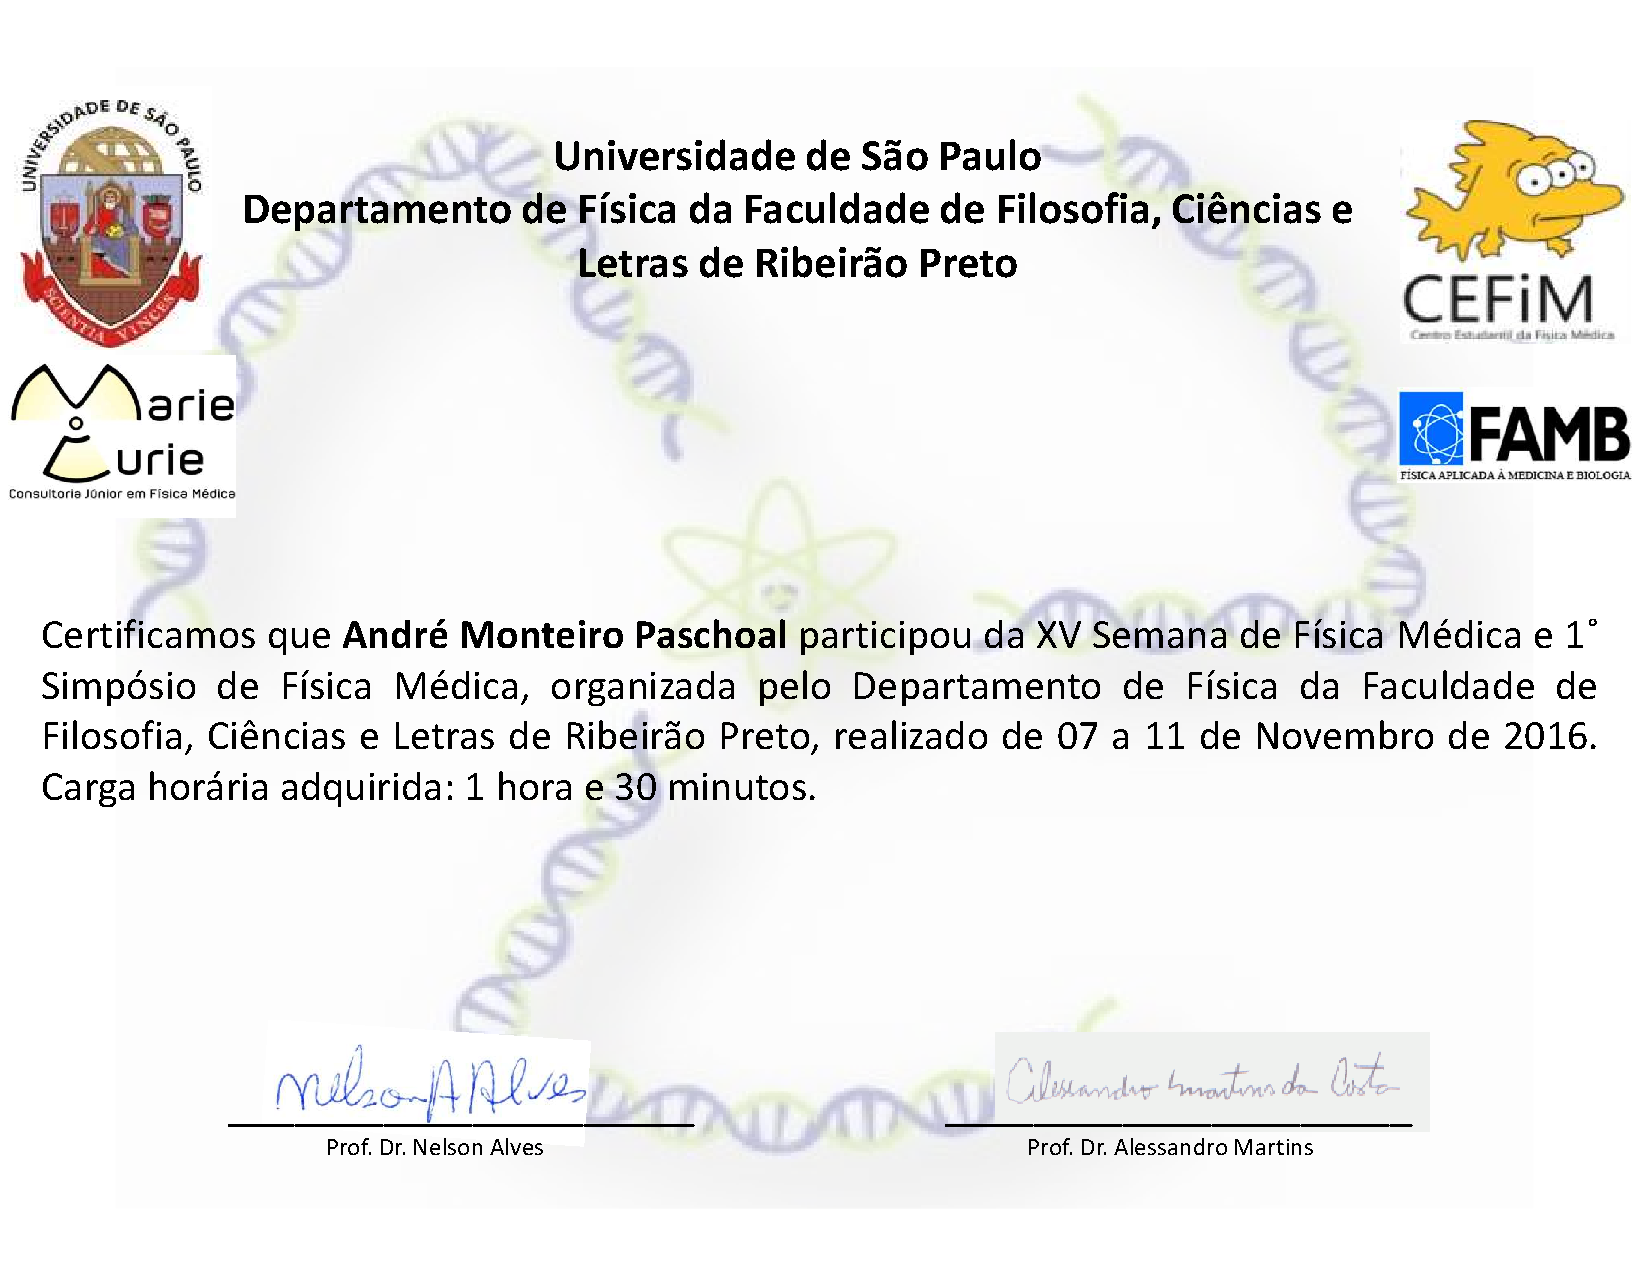
\includepdf[pages=-, scale=1,pagecommand=\thispagestyle{empty}]{\detokenize{Diplomas/certificadoSFM2016}}

\newpage
\subsection{Participa\c{c}\~{a}o em Eventos Cient\'{\i}ficos (com apresenta\c{c}\~{a}o de trabalho ou oferecimento de cursos, palestras ou debates}
\label{certificados:CBFM2017}
Esta subseção apresenta o comprovante da participação no XXII Congresso Brasileiro de Física Médica com seus respectivos propósitos.
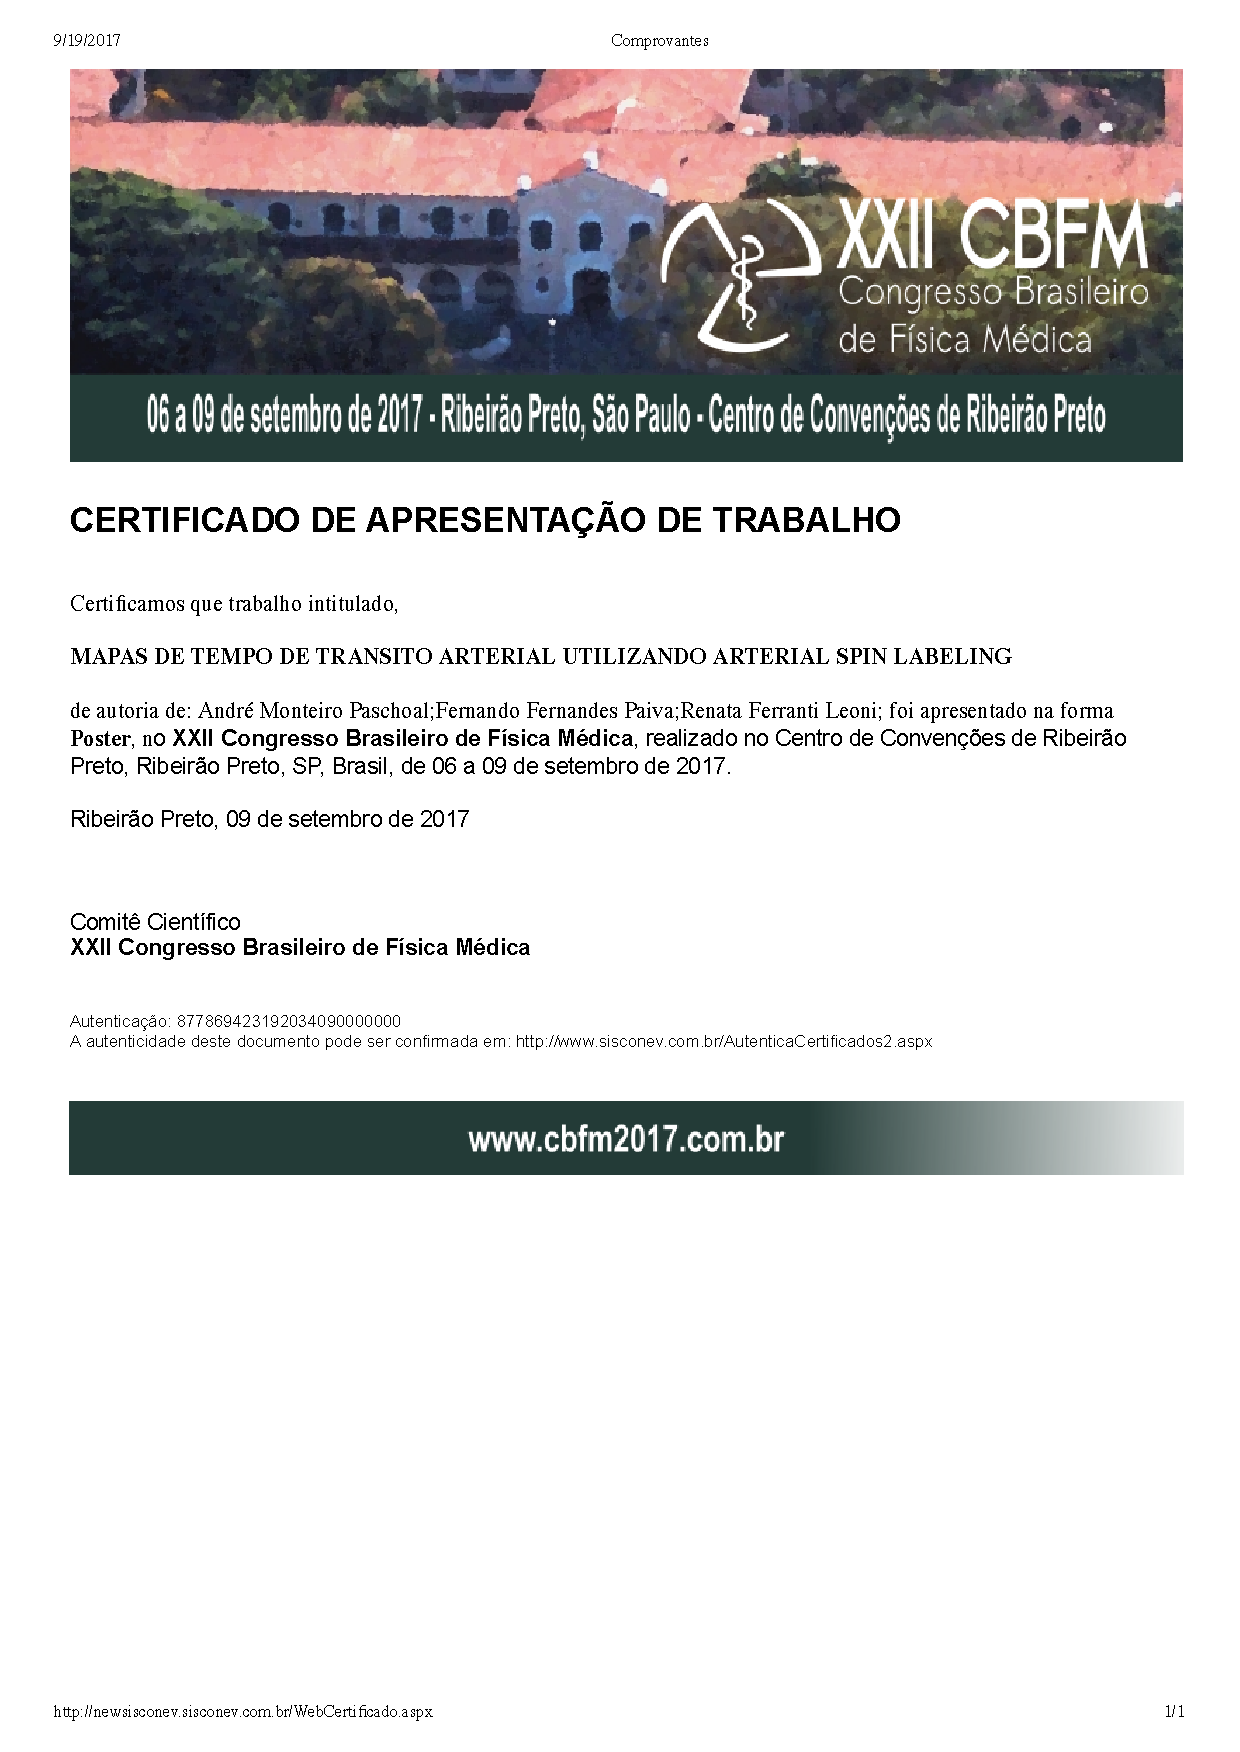
\includepdf[pages=-, scale=1,pagecommand=\thispagestyle{empty}]{\detokenize{Diplomas/certificadoCBFM2017}}

\newpage
\subsection{Participa\c{c}\~{a}o em Eventos Cient\'{\i}ficos (com apresenta\c{c}\~{a}o de trabalho ou oferecimento de cursos, palestras ou debates}
\label{certificados:FAMB2017}
Esta subseção apresenta o comprovante da participação no Seminário semanal do programa de Física Aplicada à Medicina e Biologia com seus respectivos propósitos.
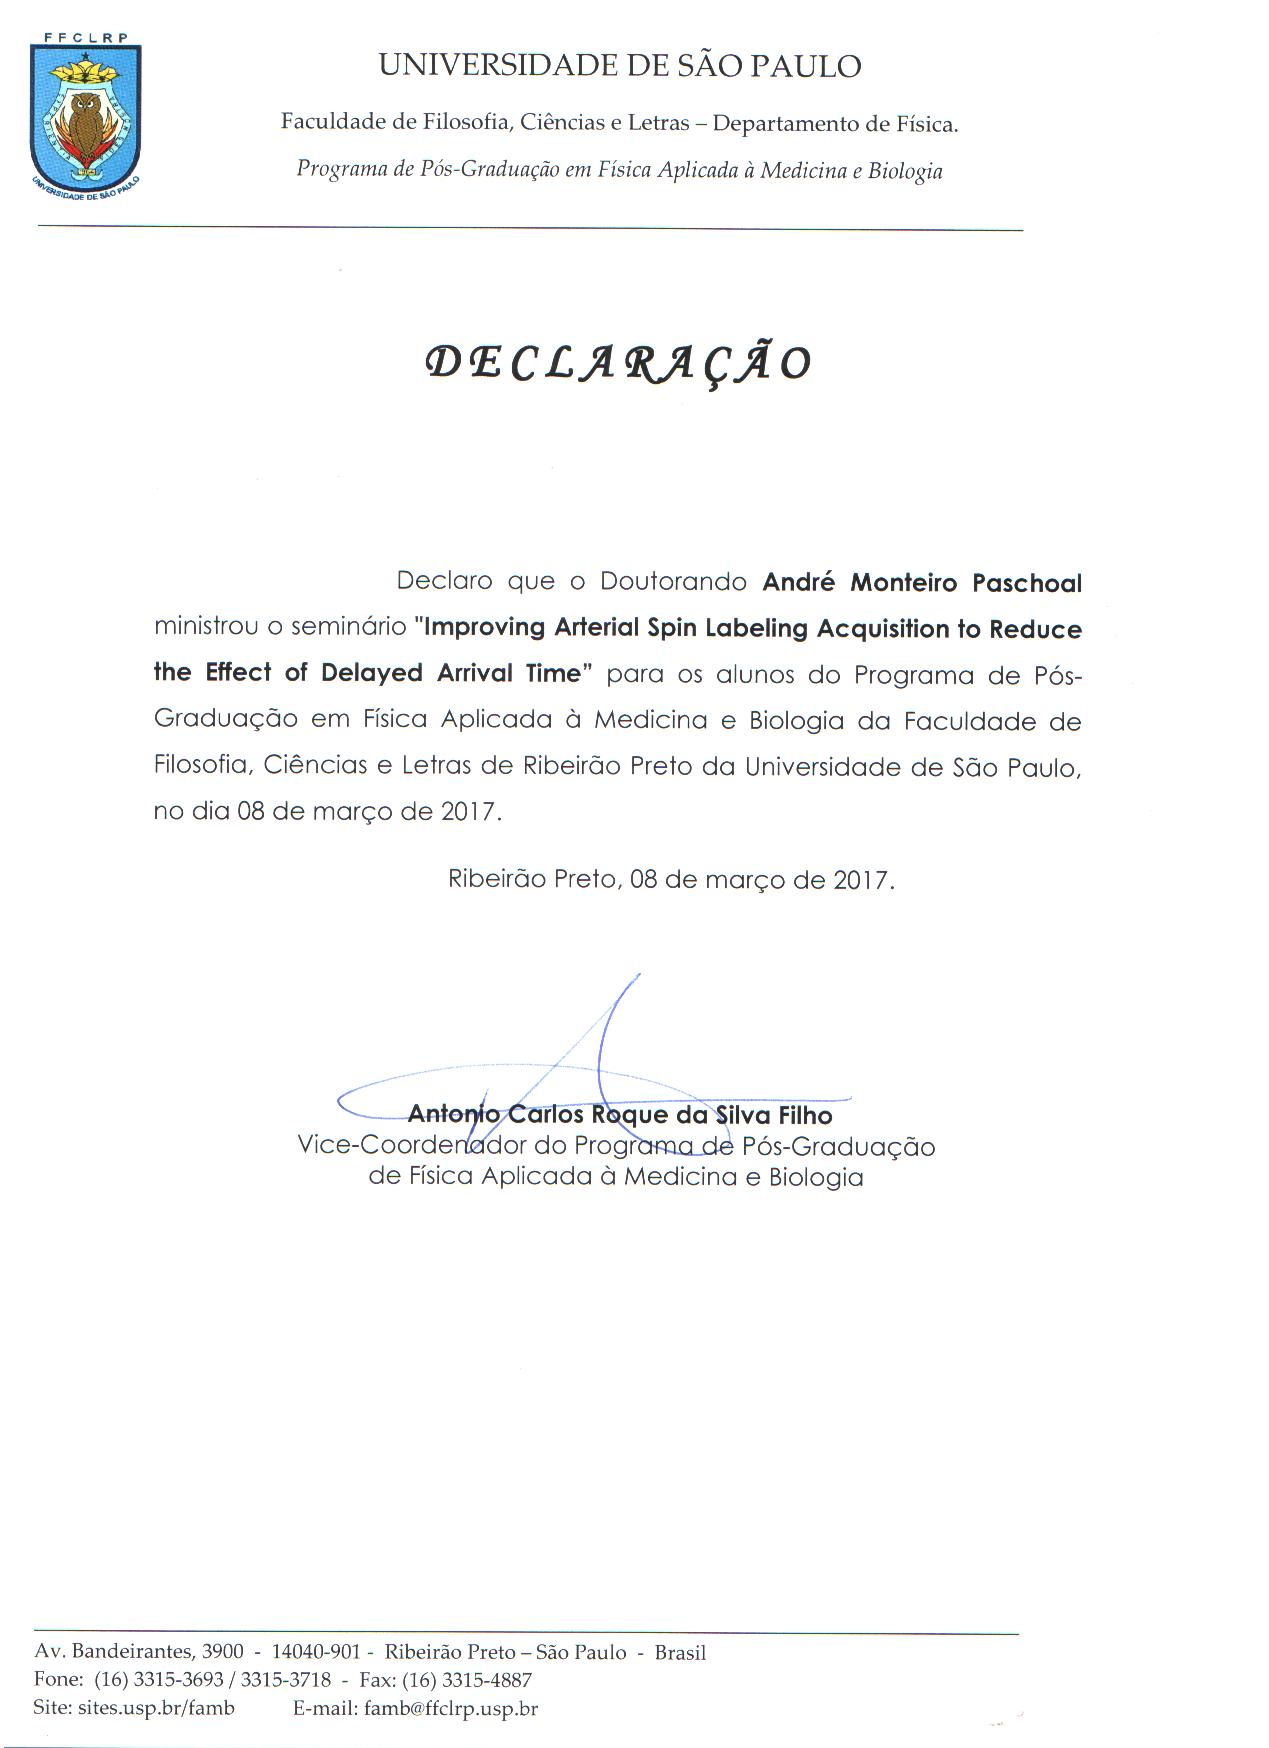
\includepdf[pages=-, scale=1,pagecommand=\thispagestyle{empty}]{\detokenize{Diplomas/CertificadoApresentacaoSeminarioFAMB}}

\newpage
\subsection{Participa\c{c}\~{a}o em Eventos Cient\'{\i}ficos (com apresenta\c{c}\~{a}o de trabalho ou oferecimento de cursos, palestras ou debates}
\label{certificados:Neuromat}
Esta subseção apresenta o comprovante da participação na palestra ``O Cérebro estatístico: desafios científicos do CEPID NeuroMat'' com seus respectivos propósitos.
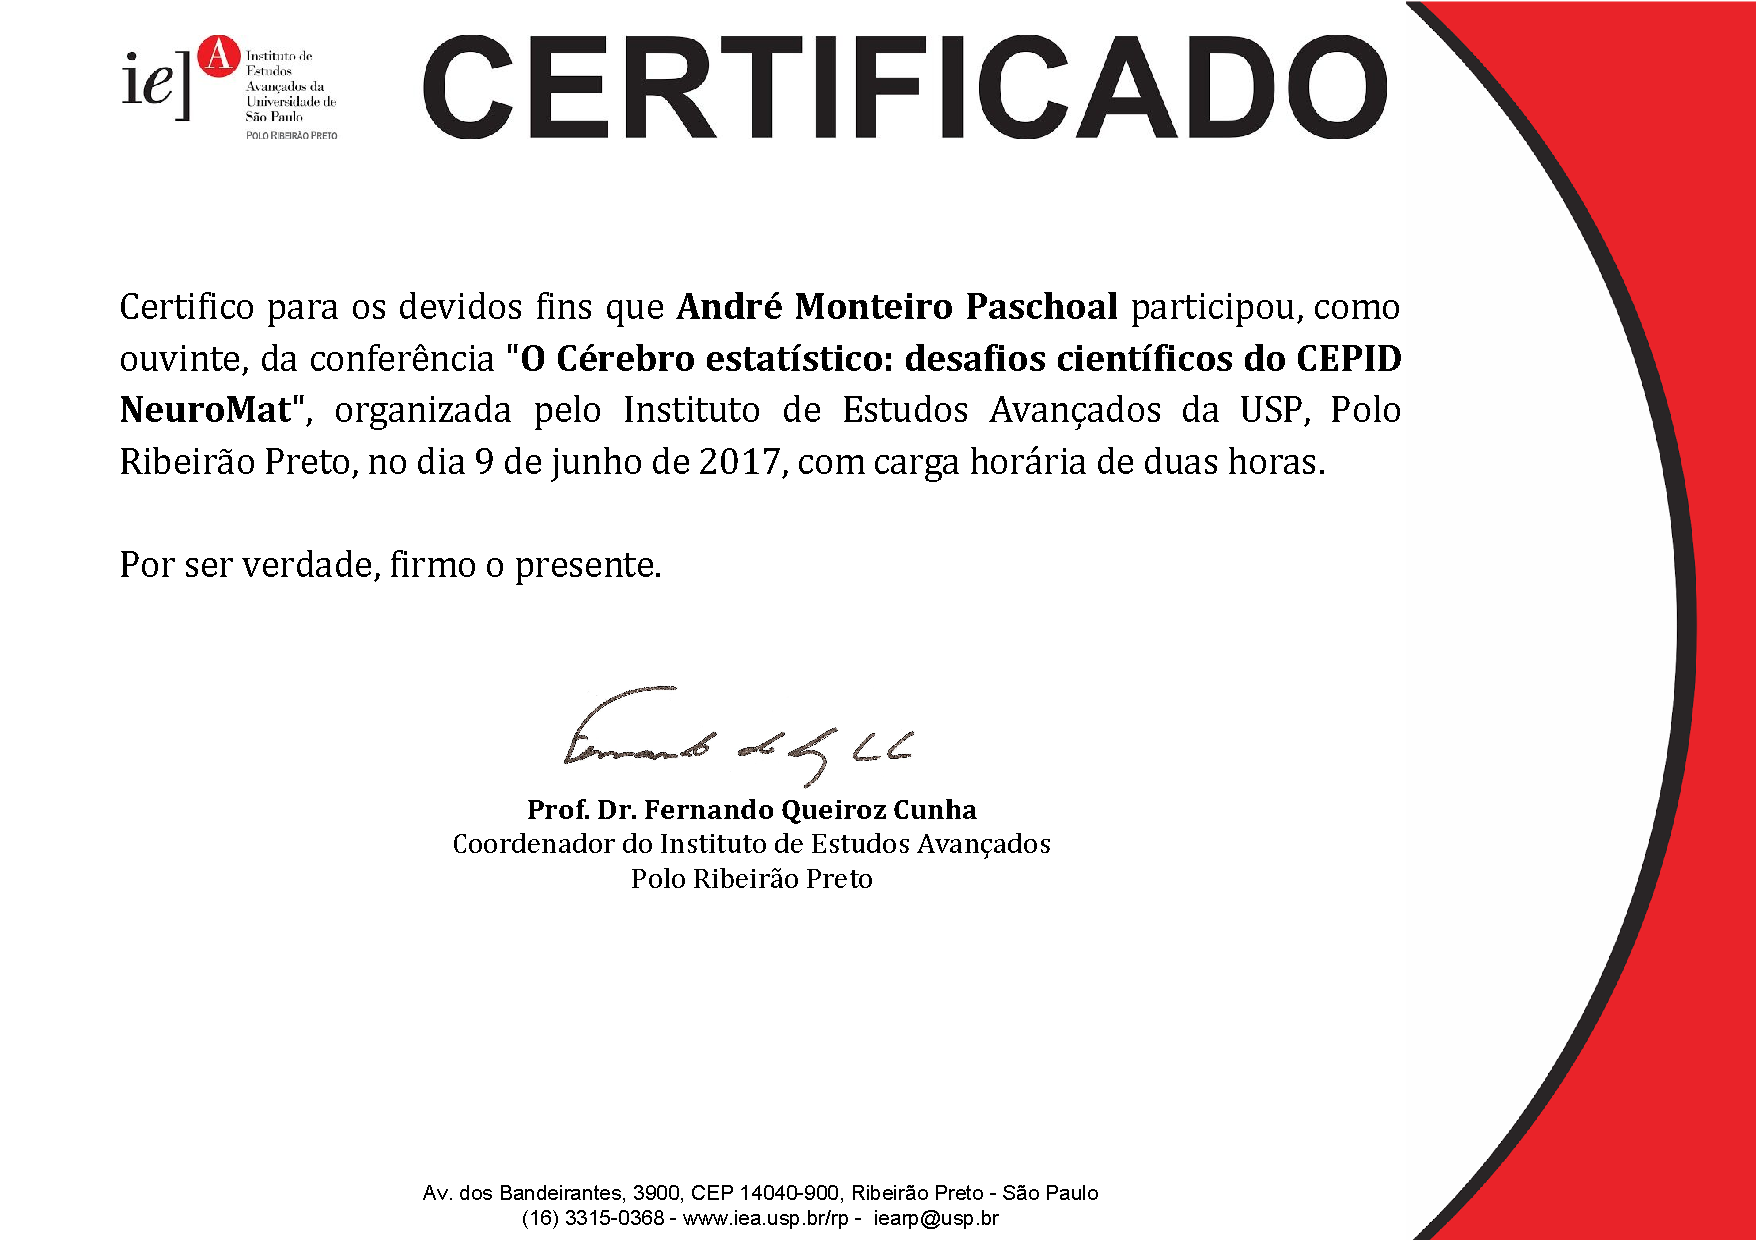
\includepdf[pages=-, scale=1,pagecommand=\thispagestyle{empty}]{\detokenize{Diplomas/Neutomat_06_2017}}

\newpage
\subsection{Participa\c{c}\~{a}o em Eventos Cient\'{\i}ficos (com apresenta\c{c}\~{a}o de trabalho ou oferecimento de cursos, palestras ou debates}
\label{certificados:SIIM2017}
Esta subseção apresenta o comprovante da participação no  8º Simpósio de Instrumentação e Imagens Médicas (SIIM) e 7º Simpósio de Processamento de Sinais (SPS) com seus respectivos propósitos.
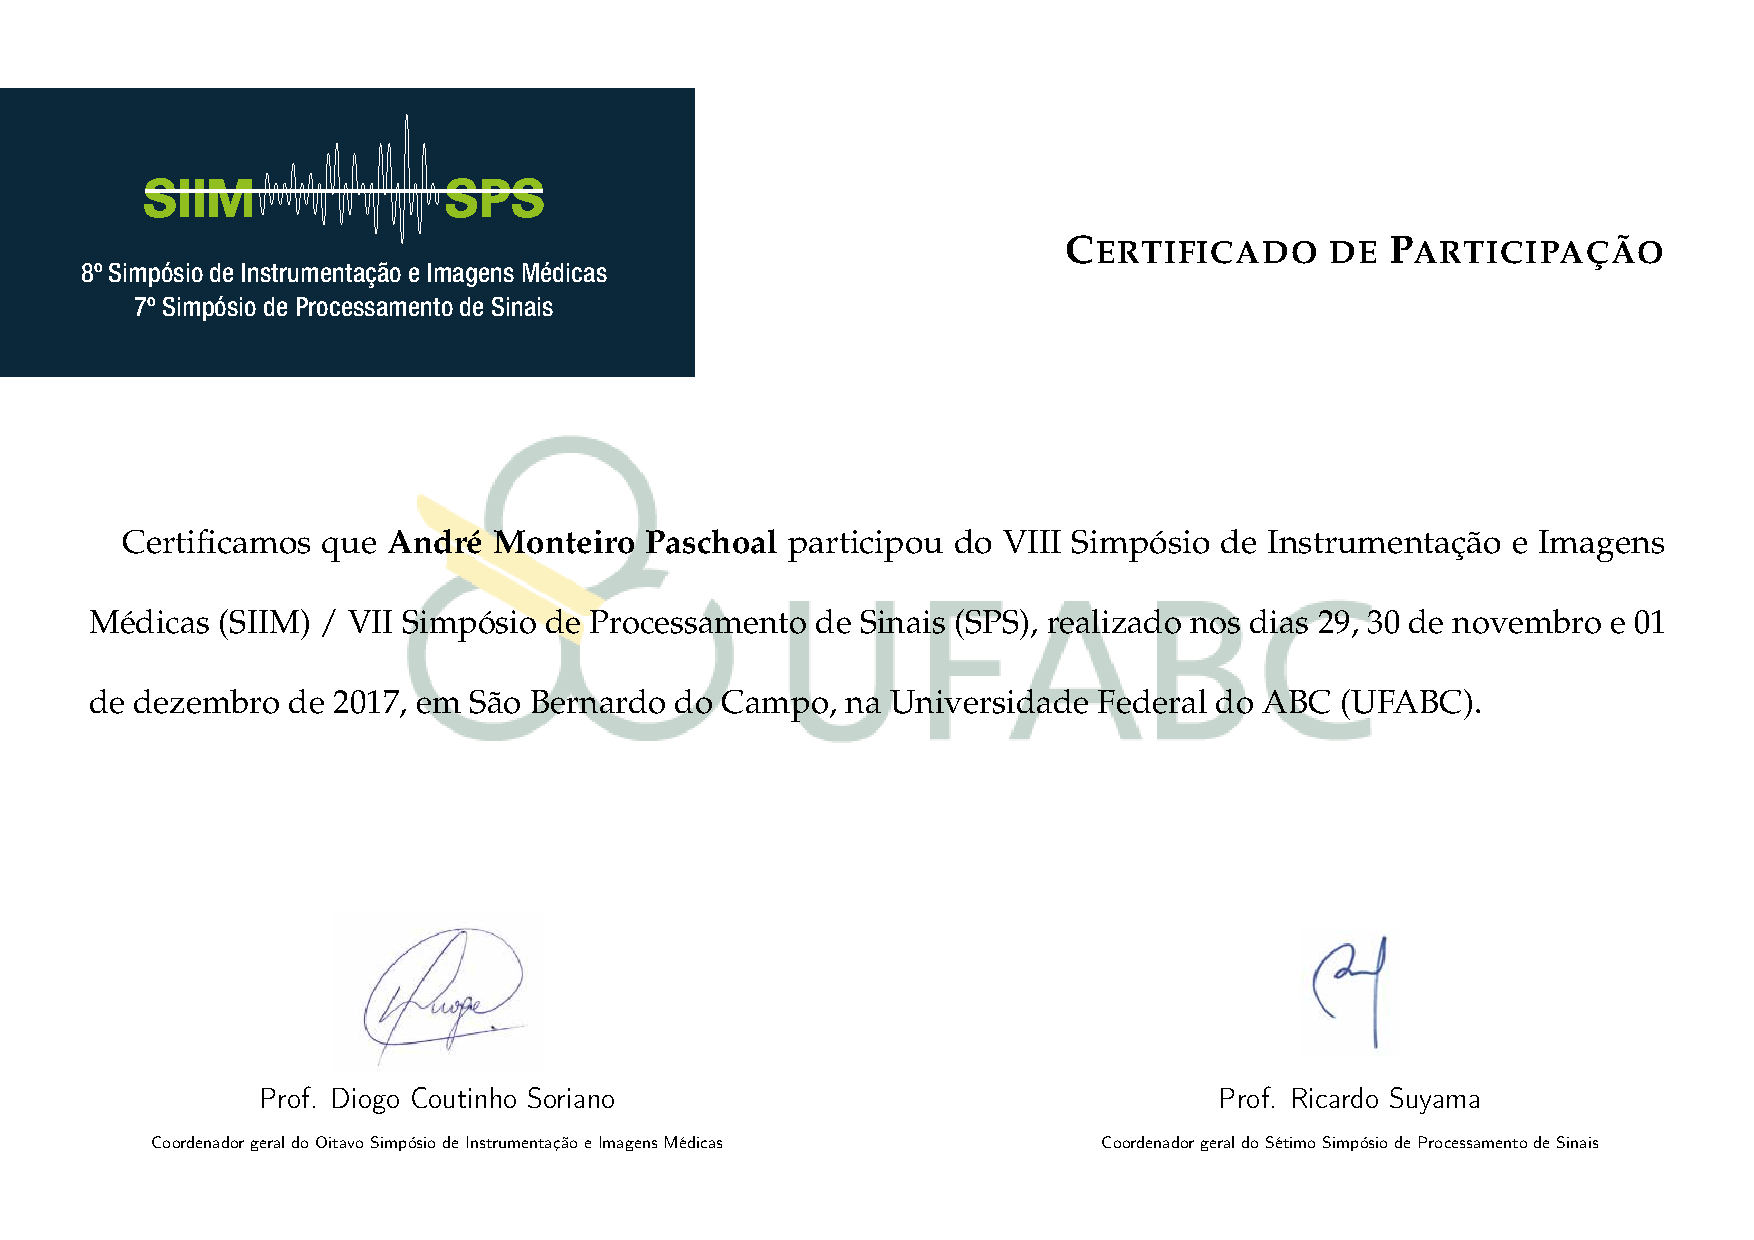
\includepdf[pages=-, scale=1,pagecommand=\thispagestyle{empty}]{\detokenize{Diplomas/SIIM2017}}

\newpage
\subsection{Participa\c{c}\~{a}o em Eventos Cient\'{\i}ficos (com apresenta\c{c}\~{a}o de trabalho ou oferecimento de cursos, palestras ou debates}
\label{certificados:ISMRM2017}
Esta subseção apresenta o comprovante da participação no 
ISMRM 25th Annual Meeting \& Exhibition com seus respectivos propósitos. \\
Obs: Ese congresso não emite certificado de apresentação de trabalhos, apenas de participação no evento.
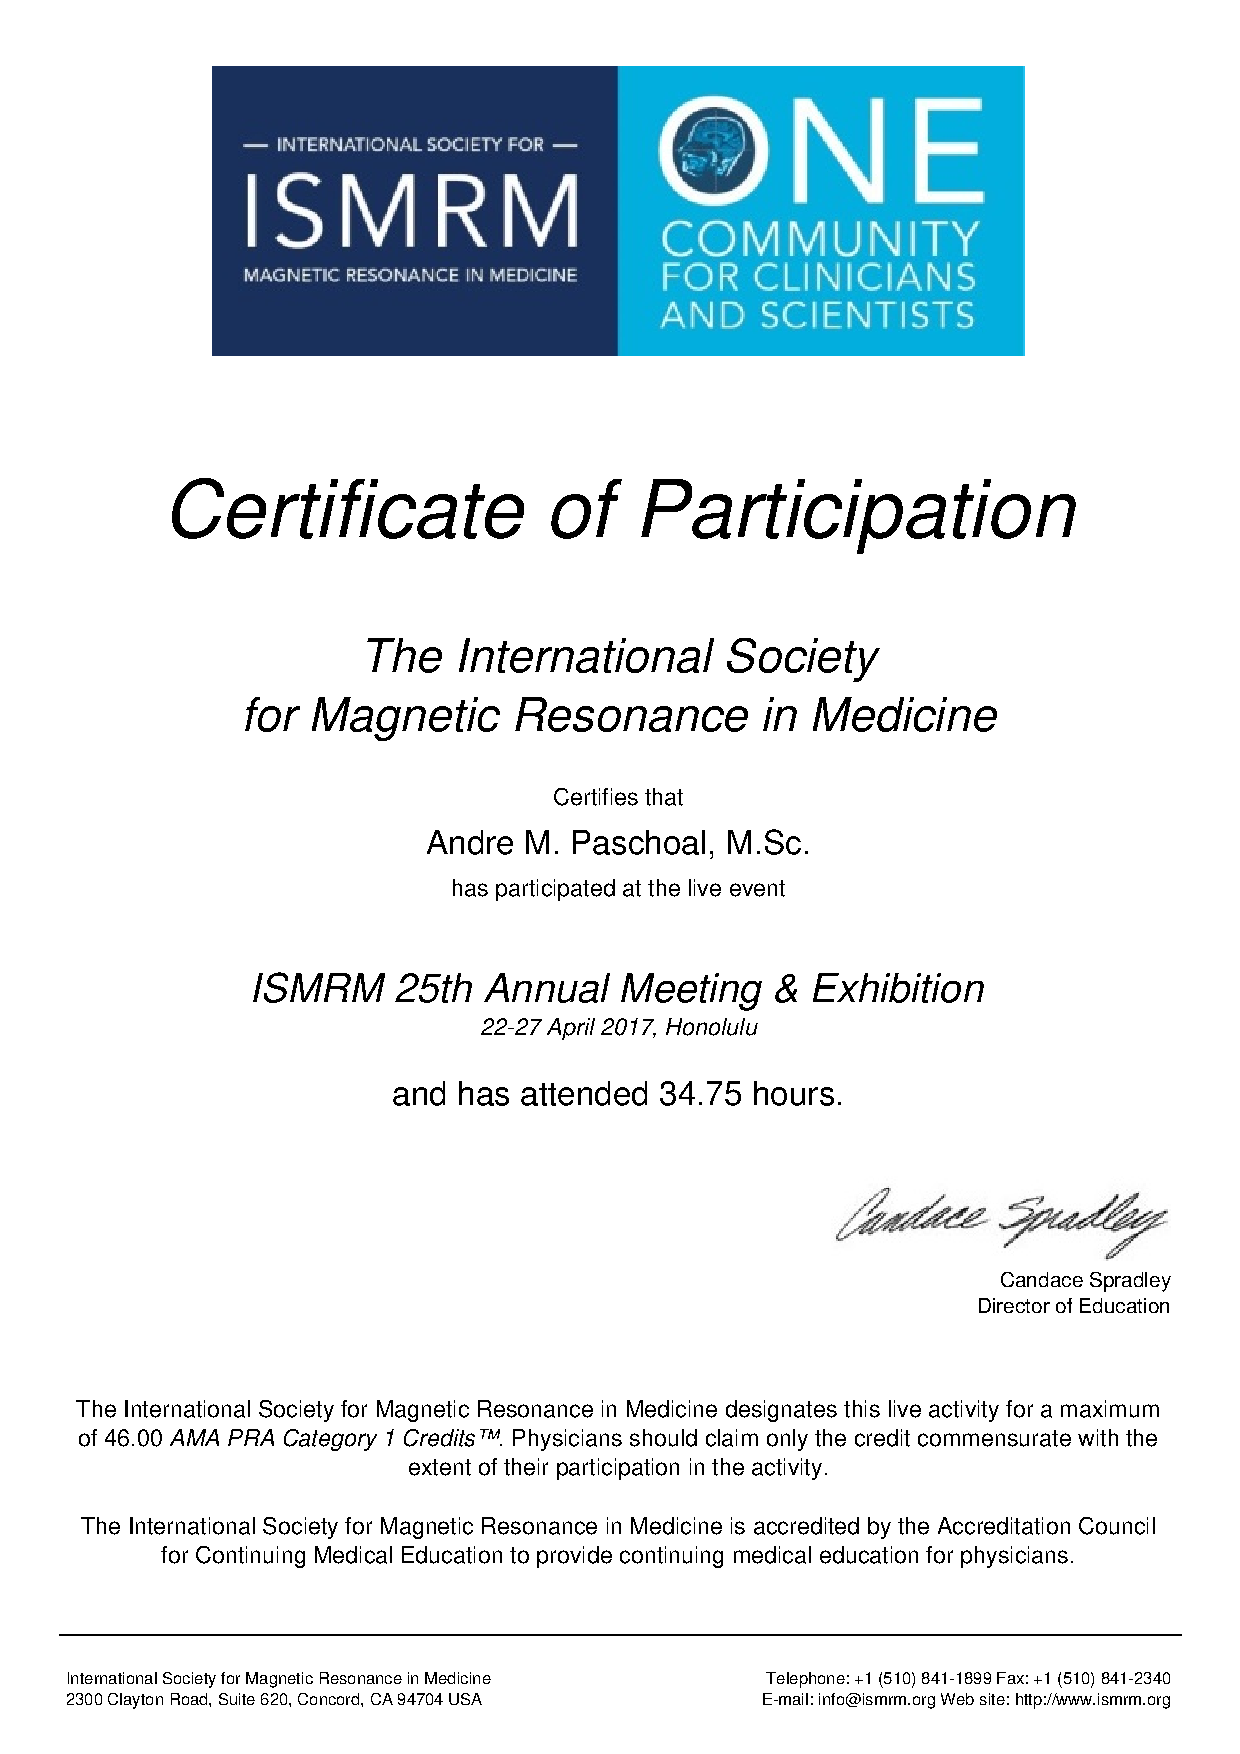
\includepdf[pages=-, scale=1,pagecommand=\thispagestyle{empty}]{\detokenize{Diplomas/ISMRM2017}}
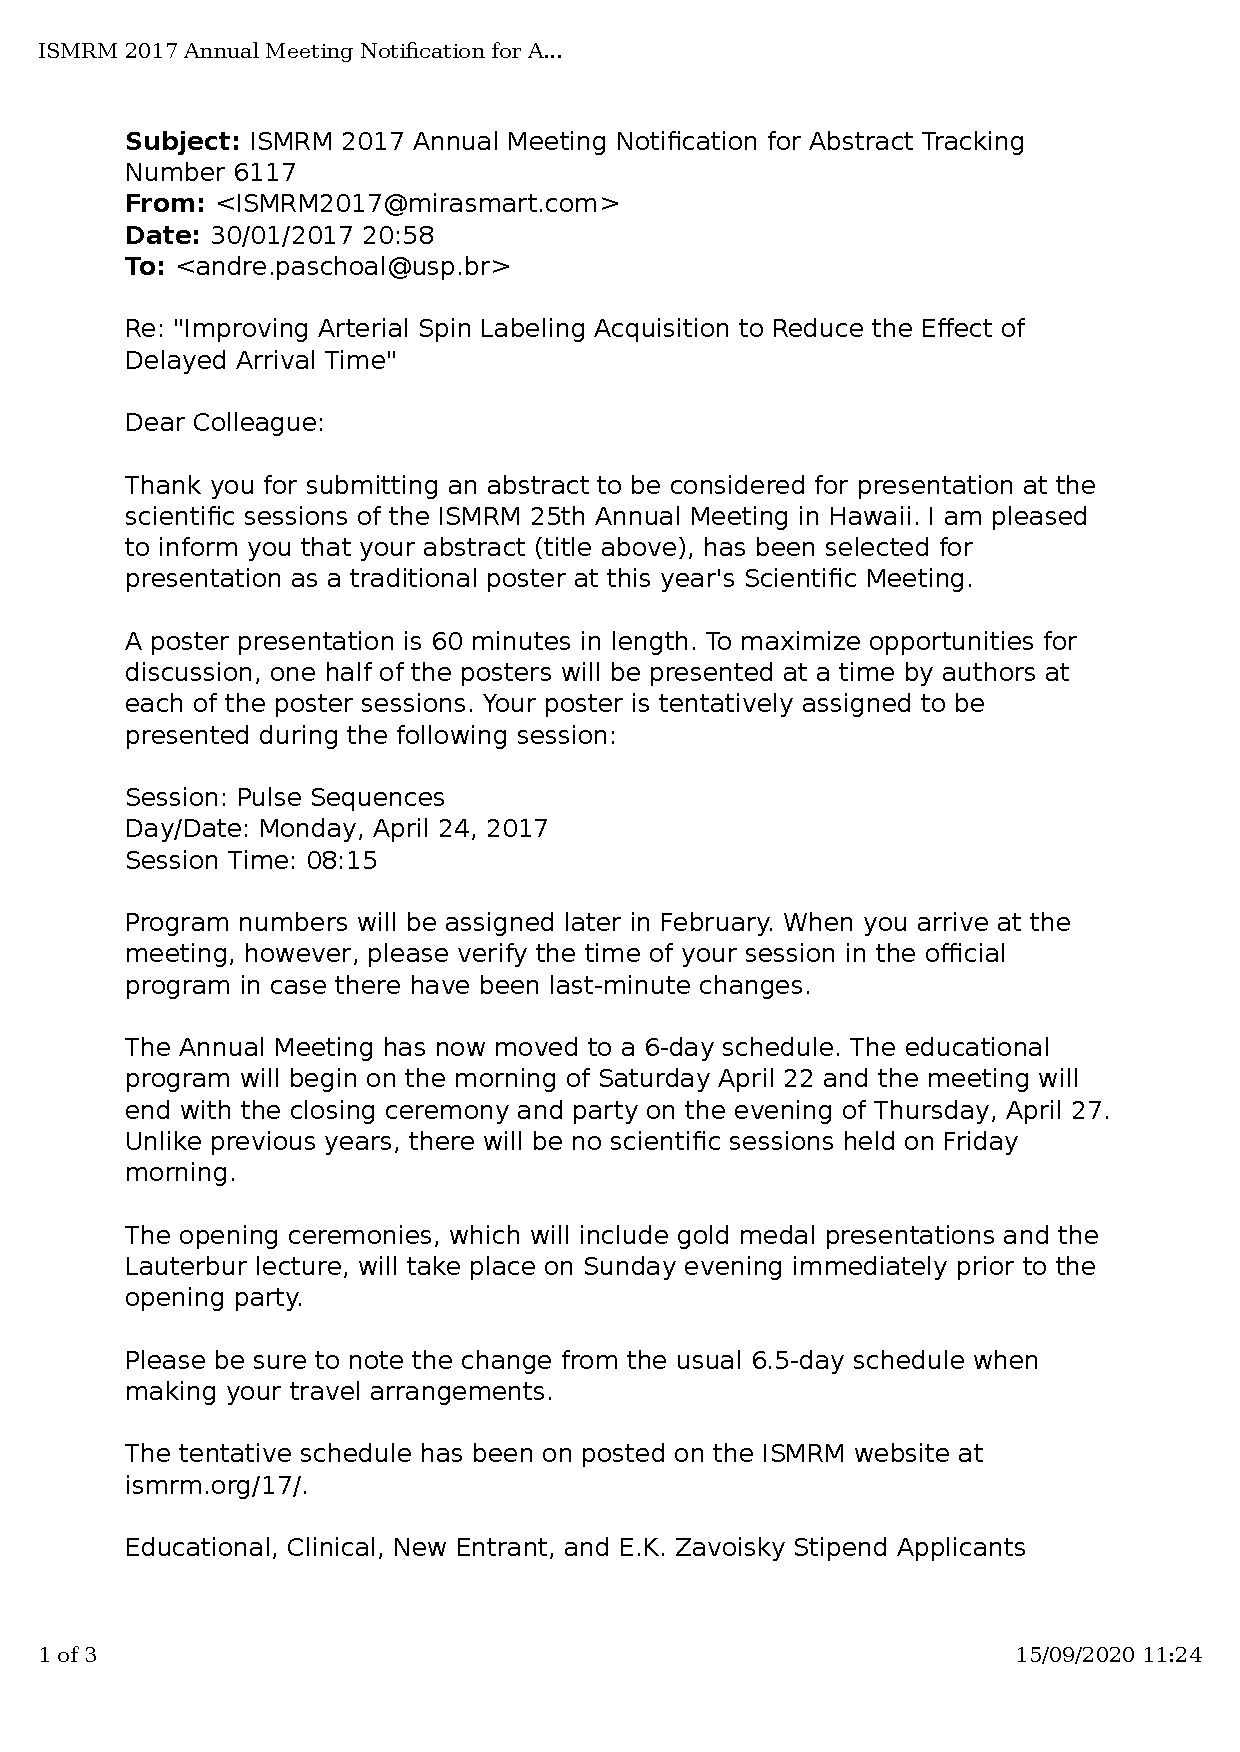
\includepdf[pages=-, scale=1,pagecommand=\thispagestyle{empty}]{\detokenize{Diplomas/AcceptanceISMRM2017}}

\newpage
\subsection{Participa\c{c}\~{a}o em Eventos Cient\'{\i}ficos (com apresenta\c{c}\~{a}o de trabalho ou oferecimento de cursos, palestras ou debates}
\label{certificados:BRAINN2017}
Esta subseção apresenta o comprovante da participação no 4º BRAINN Congress com seus respectivos propósitos.
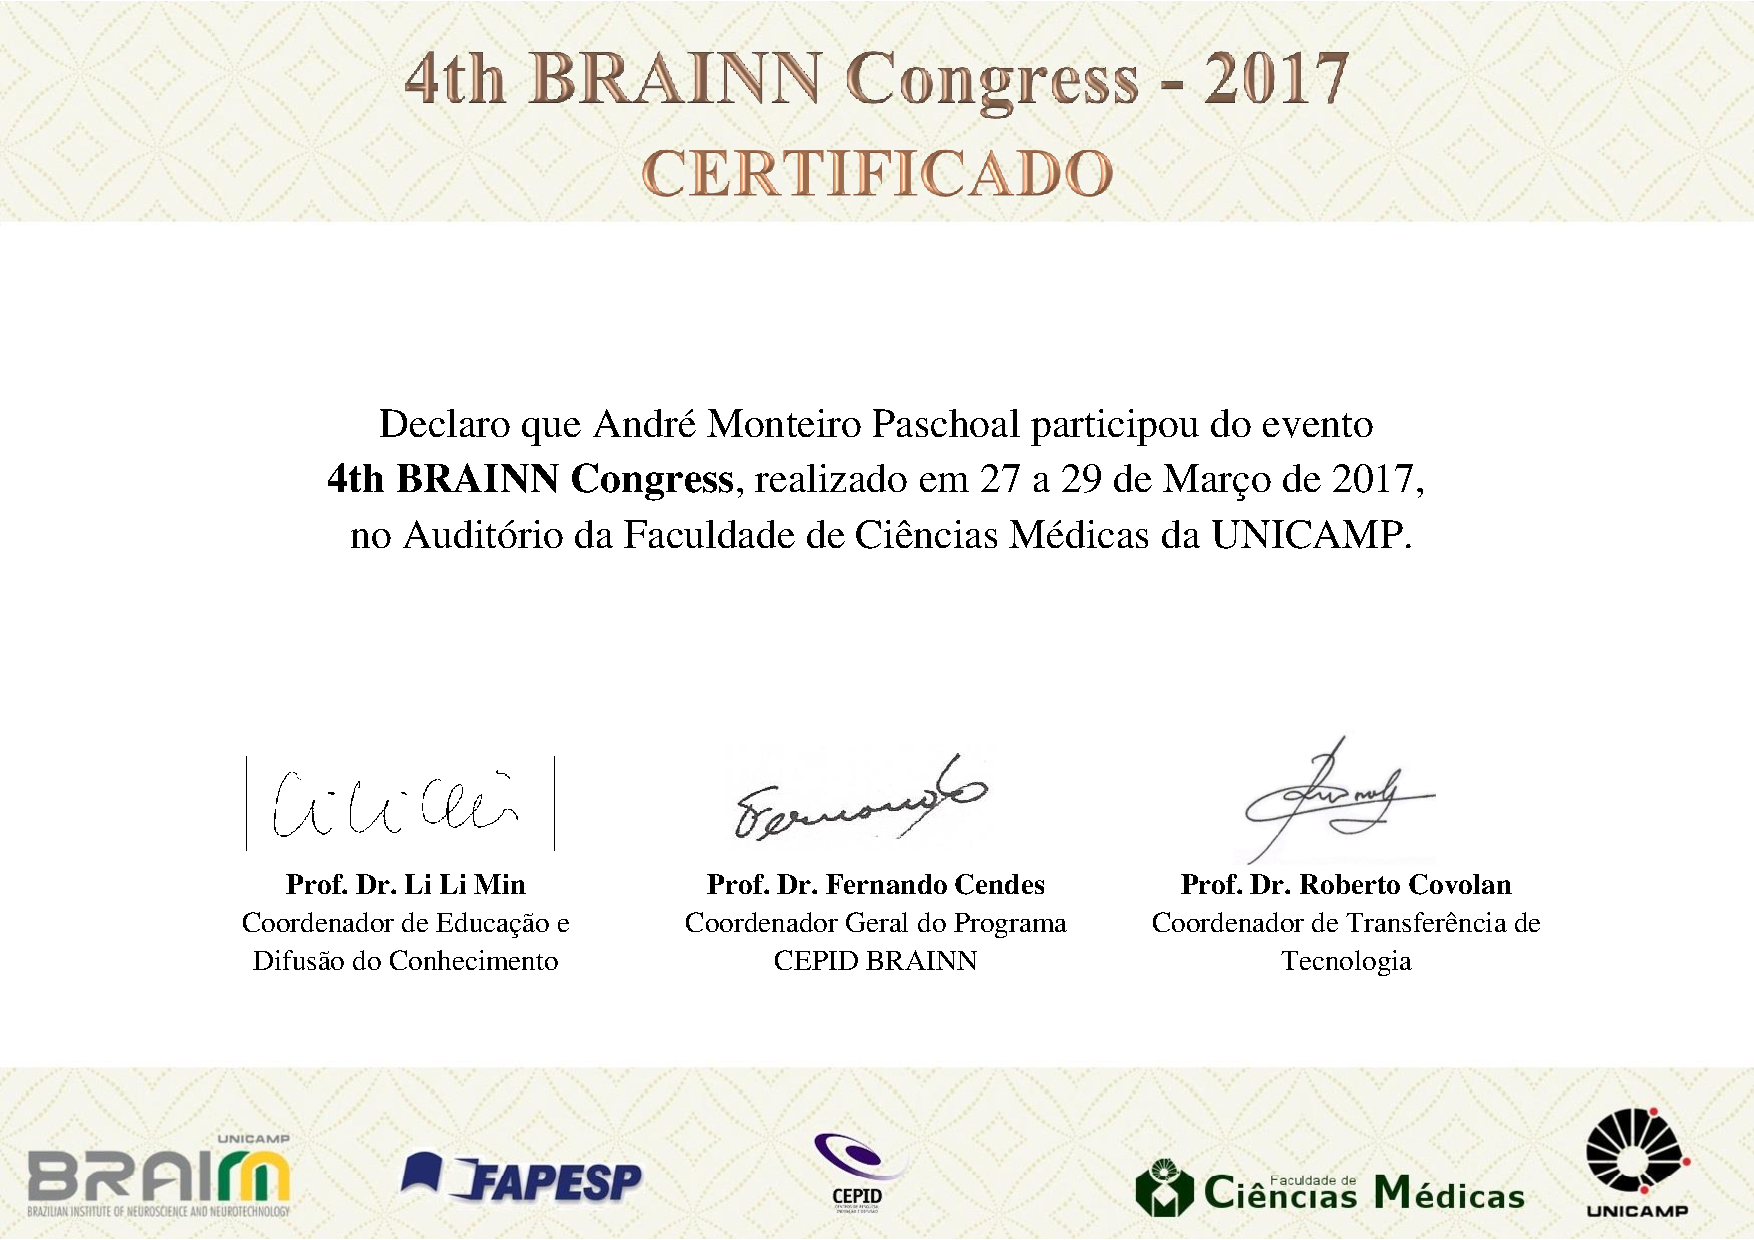
\includepdf[pages=-, scale=1,pagecommand=\thispagestyle{empty}]{\detokenize{Diplomas/BRAINN2017}}

\newpage
\subsection{Participa\c{c}\~{a}o em Eventos Cient\'{\i}ficos (com apresenta\c{c}\~{a}o de trabalho ou oferecimento de cursos, palestras ou debates}
\label{certificados:BRAINN2018}
Esta subseção apresenta o comprovante da participação no 5º BRAINN Congress com seus respectivos propósitos.
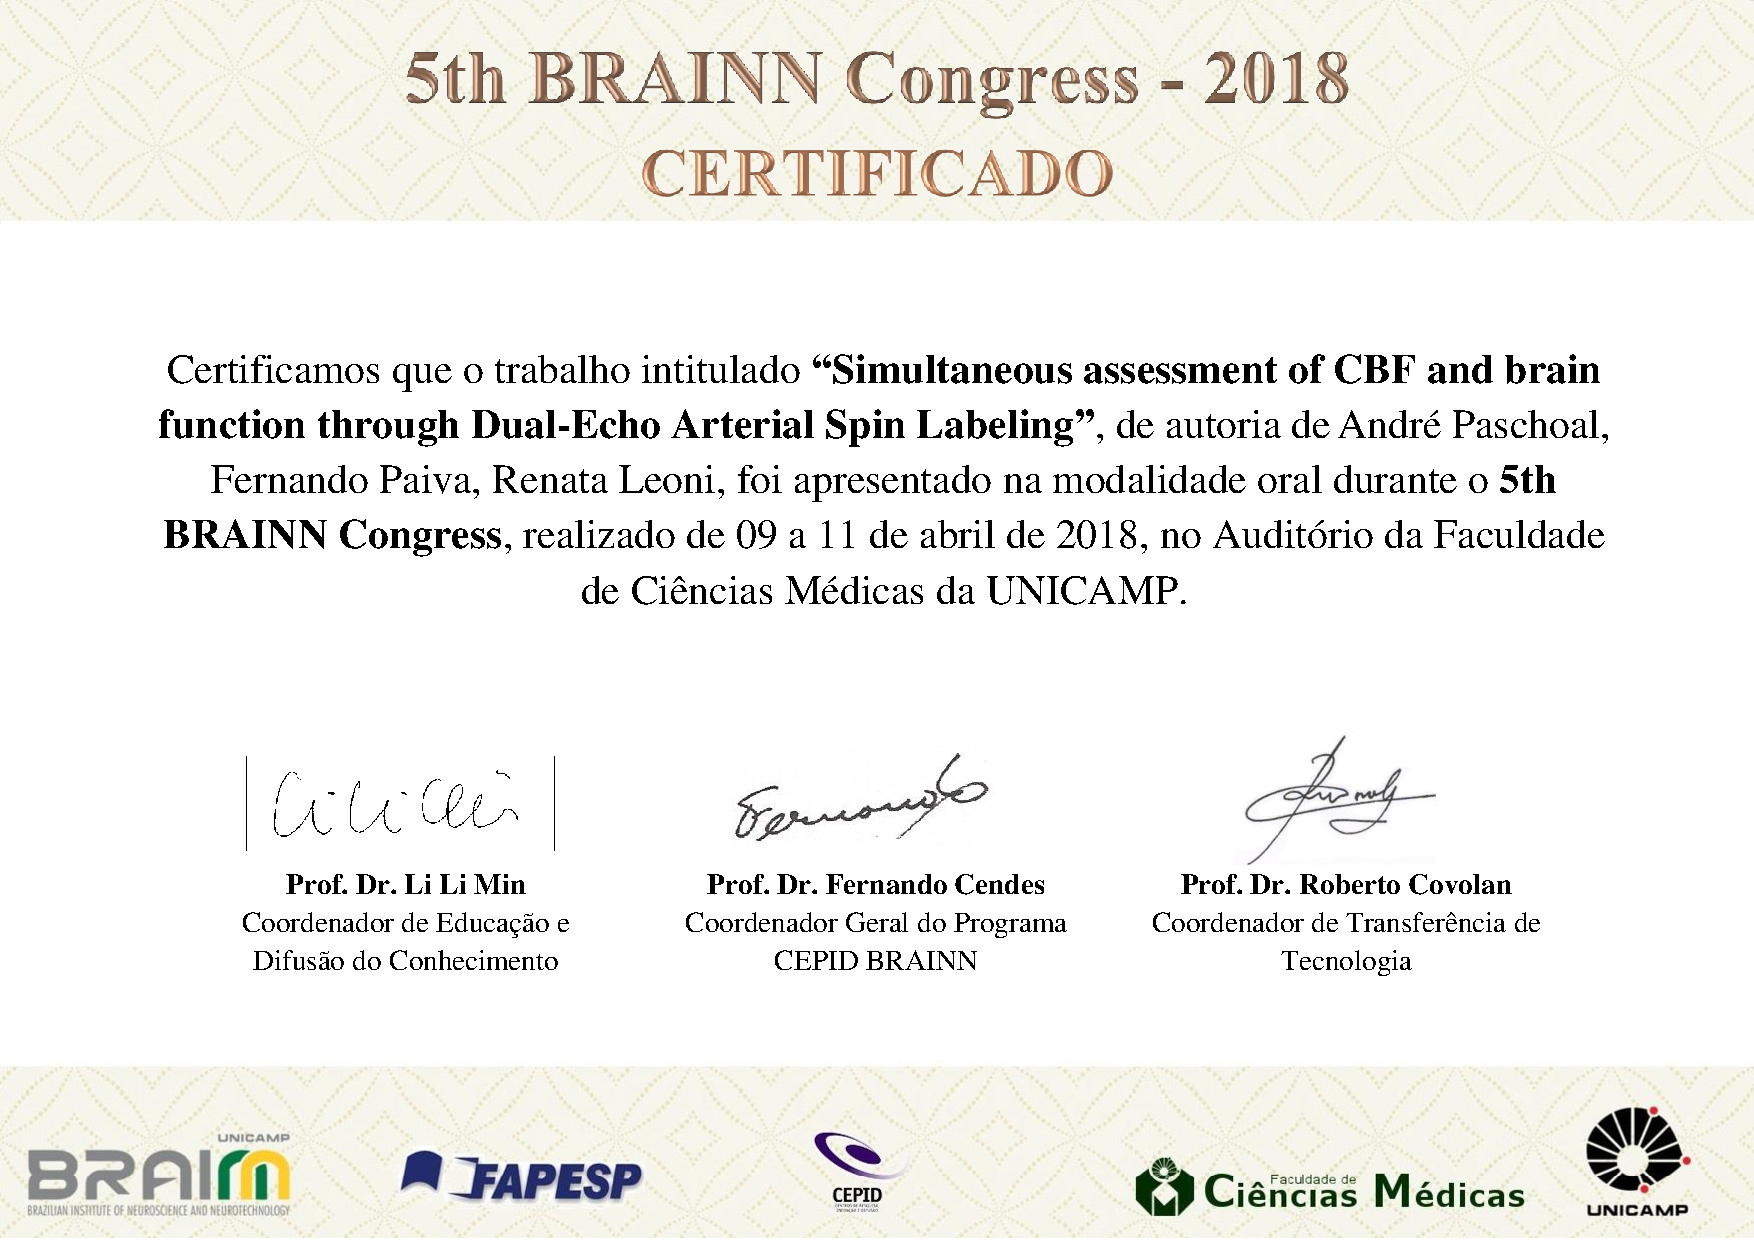
\includepdf[pages=-, scale=1,pagecommand=\thispagestyle{empty}]{\detokenize{Diplomas/BRAINN2018_apresentacao}}

\newpage
\subsection{Participa\c{c}\~{a}o em Eventos Cient\'{\i}ficos (com apresenta\c{c}\~{a}o de trabalho ou oferecimento de cursos, palestras ou debates}
\label{certificados:BRAINN2018_2}
Esta subseção apresenta o resumo publicado nos anais do 5º BRAINN Congress com seus respectivos propósitos.
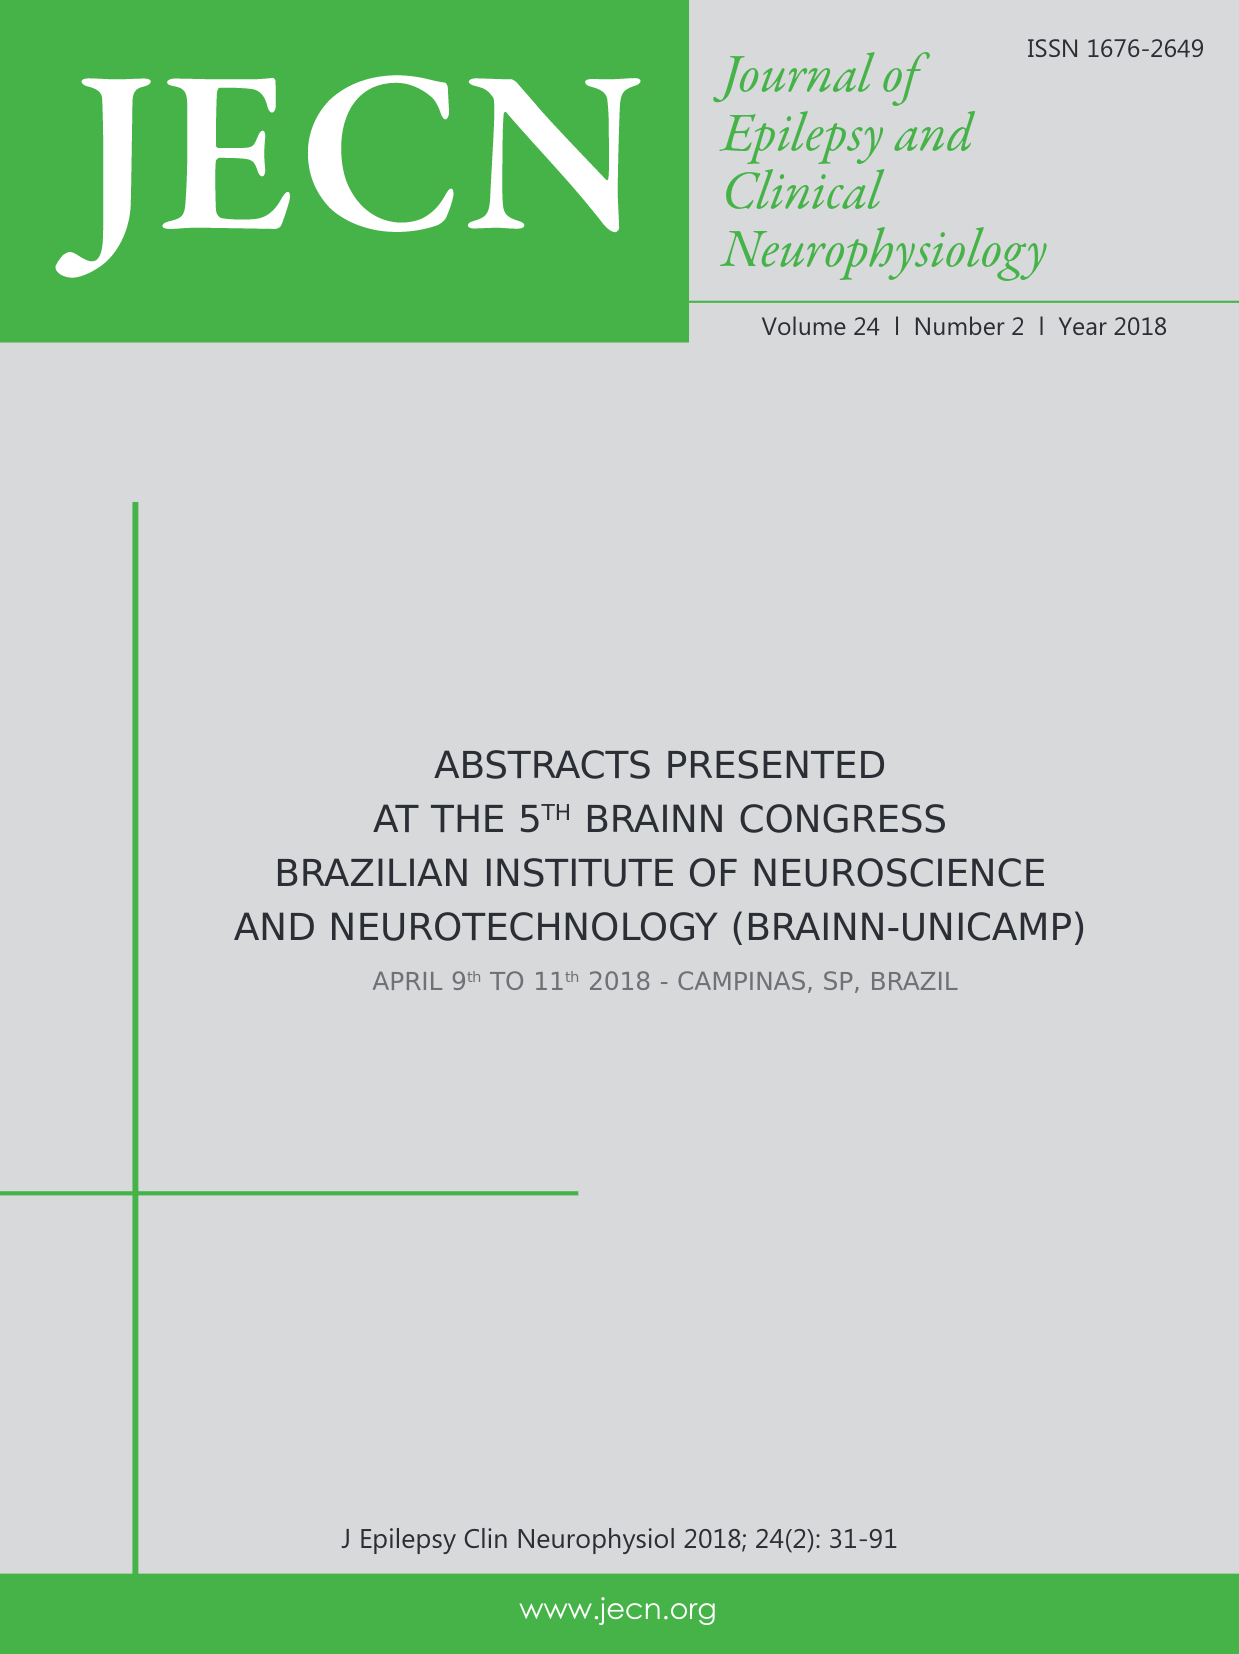
\includepdf[pages=-, scale=1,pagecommand=\thispagestyle{empty}]{\detokenize{docs/brainn2018}}

\newpage
\subsection{Participa\c{c}\~{a}o em Eventos Cient\'{\i}ficos (com apresenta\c{c}\~{a}o de trabalho ou oferecimento de cursos, palestras ou debates}
\label{certificados:ISMRM2018}
Esta subseção apresenta o comprovante da participação no Joint Annual Meeting ISMRM-ESMRMB com seus respectivos propósitos. \\
Obs: Ese congresso não emite certificado de apresentação de trabalhos, apenas de participação no evento.
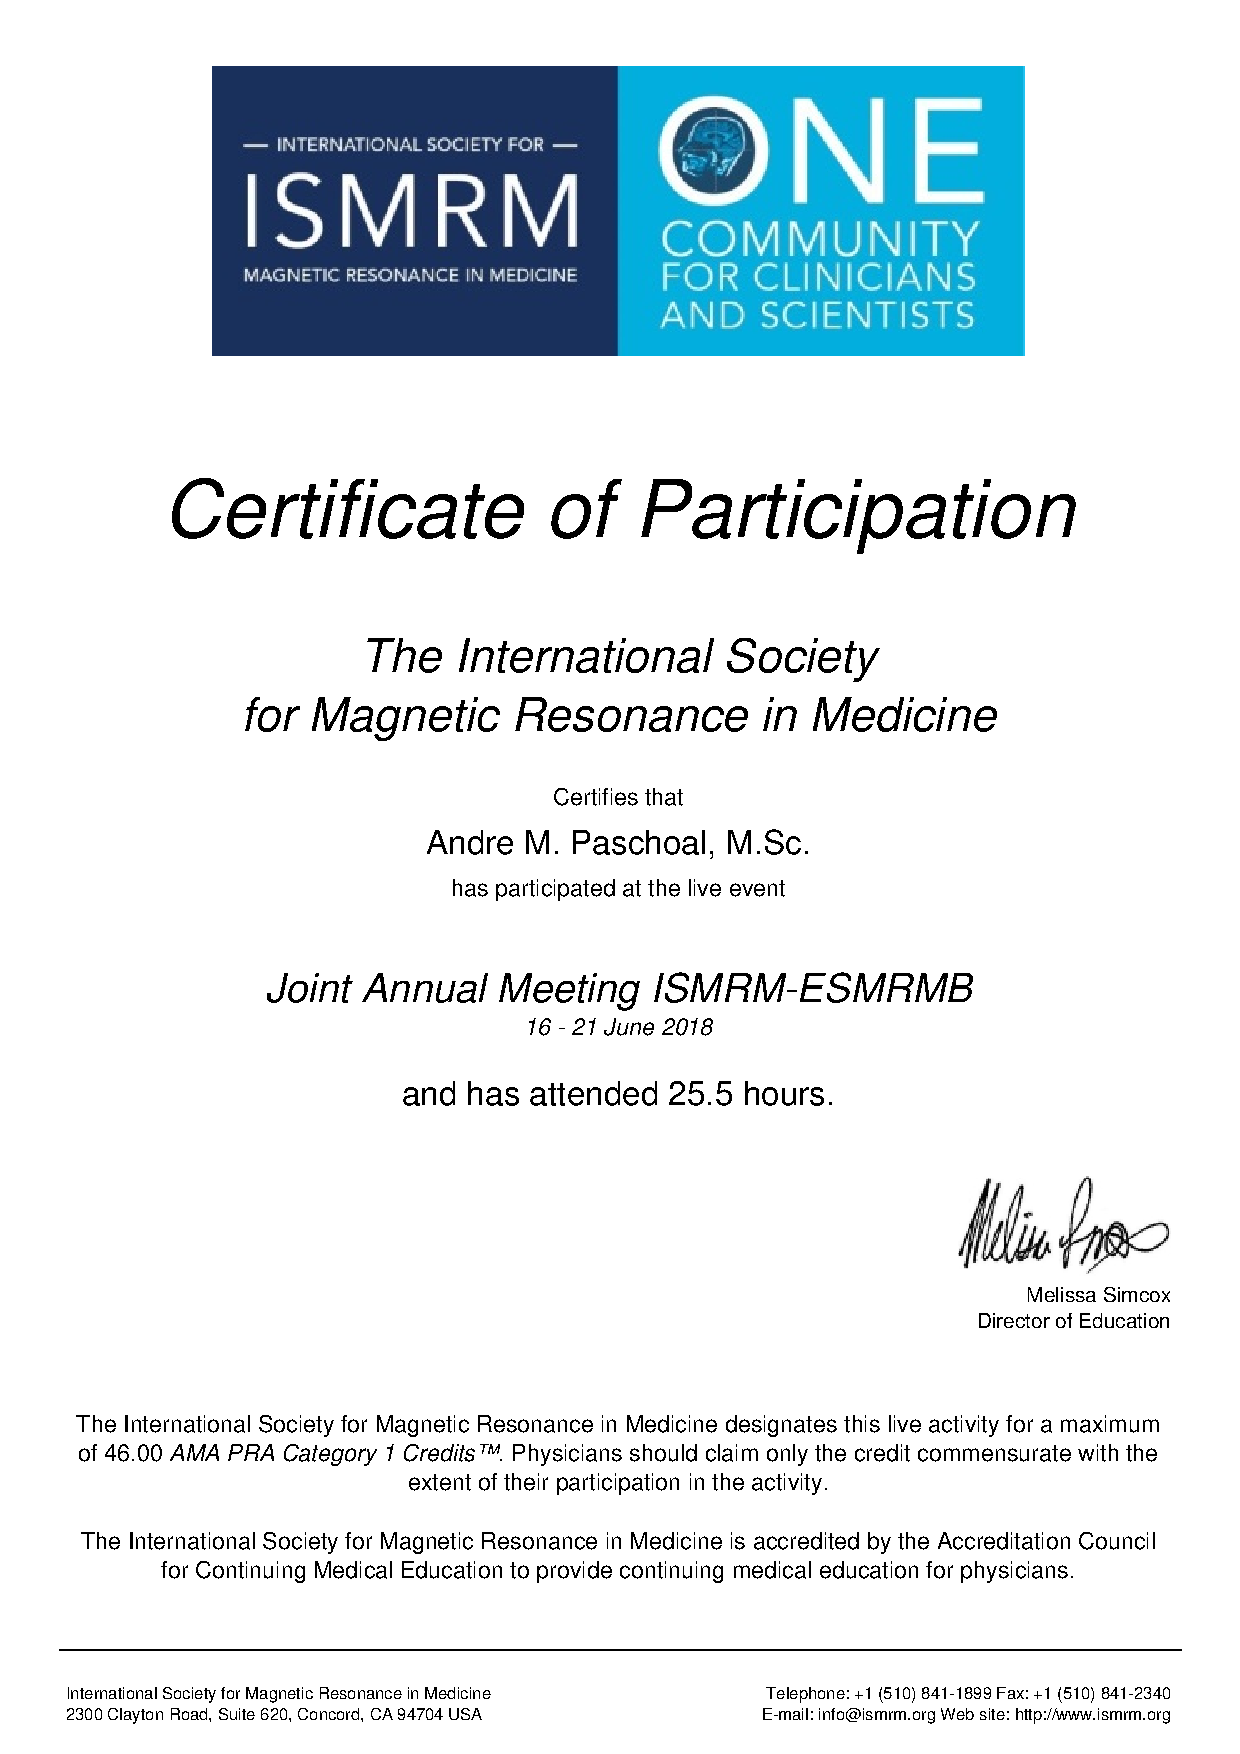
\includepdf[pages=-, scale=1,pagecommand=\thispagestyle{empty}]{\detokenize{Diplomas/ISMRM2018}}
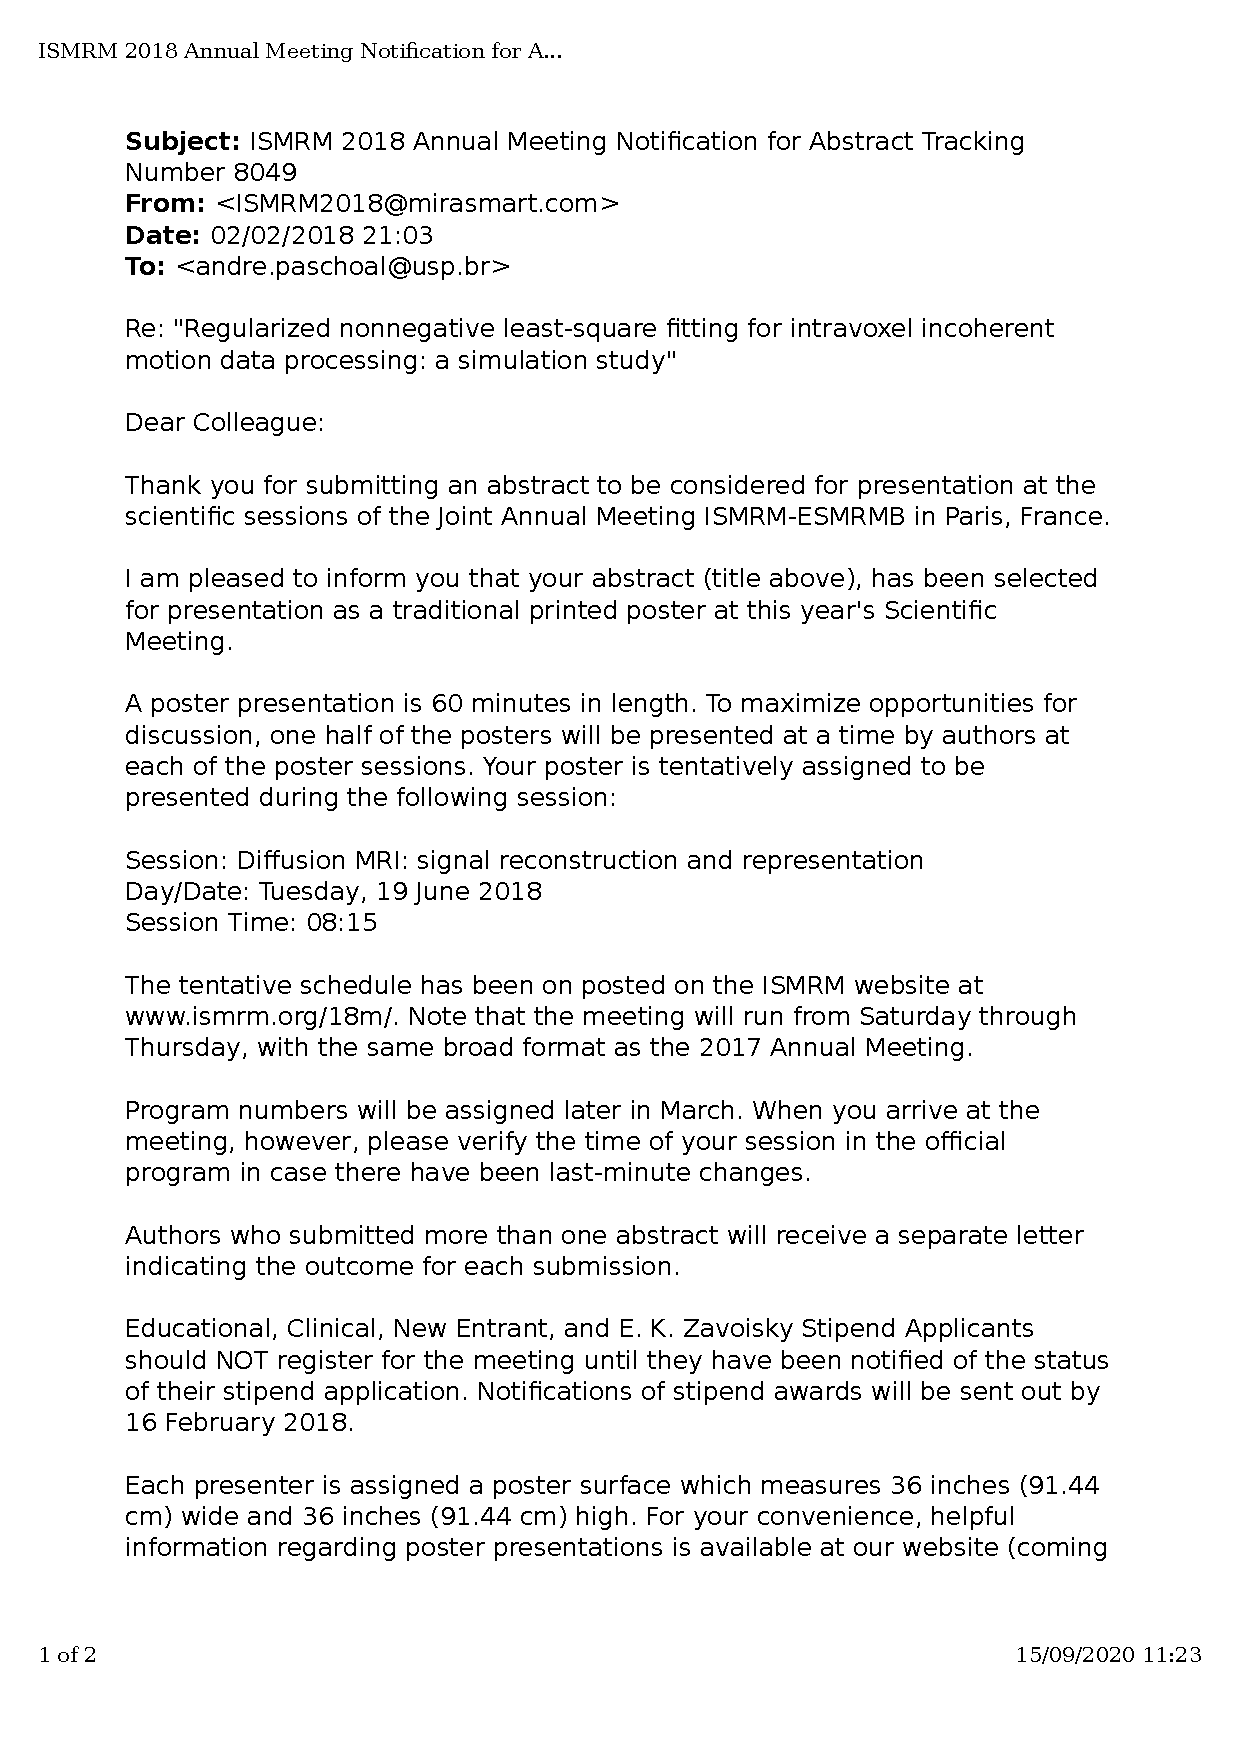
\includepdf[pages=-, scale=1,pagecommand=\thispagestyle{empty}]{\detokenize{Diplomas/AcceptanceISMRM2018_1}}
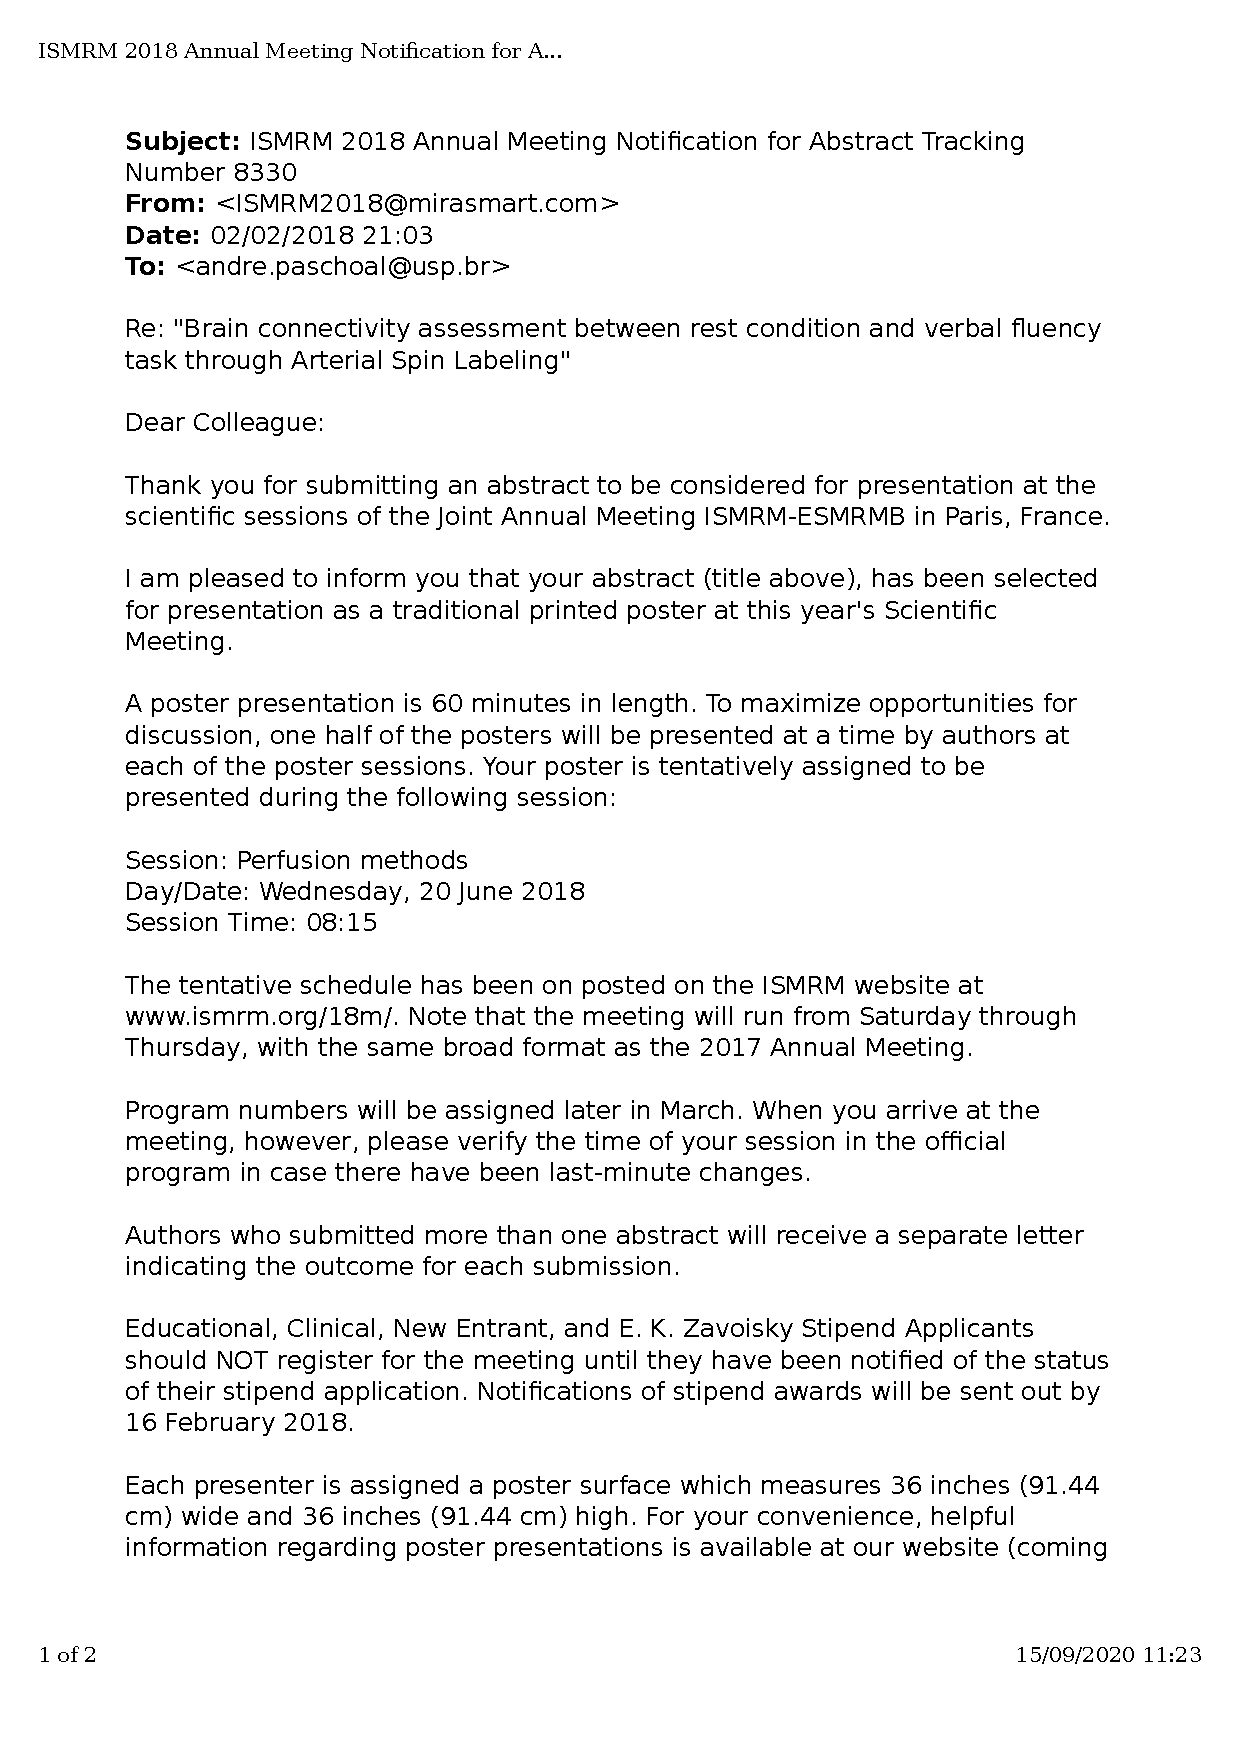
\includepdf[pages=-, scale=1,pagecommand=\thispagestyle{empty}]{\detokenize{Diplomas/AcceptanceISMRM2018_2}}


\newpage
\subsection{Participa\c{c}\~{a}o em Eventos Cient\'{\i}ficos (com apresenta\c{c}\~{a}o de trabalho ou oferecimento de cursos, palestras ou debates}
\label{certificados:SFM2017}
Esta subseção apresenta o comprovante da participação na XV Semana da Física Médica com seus respectivos propósitos.
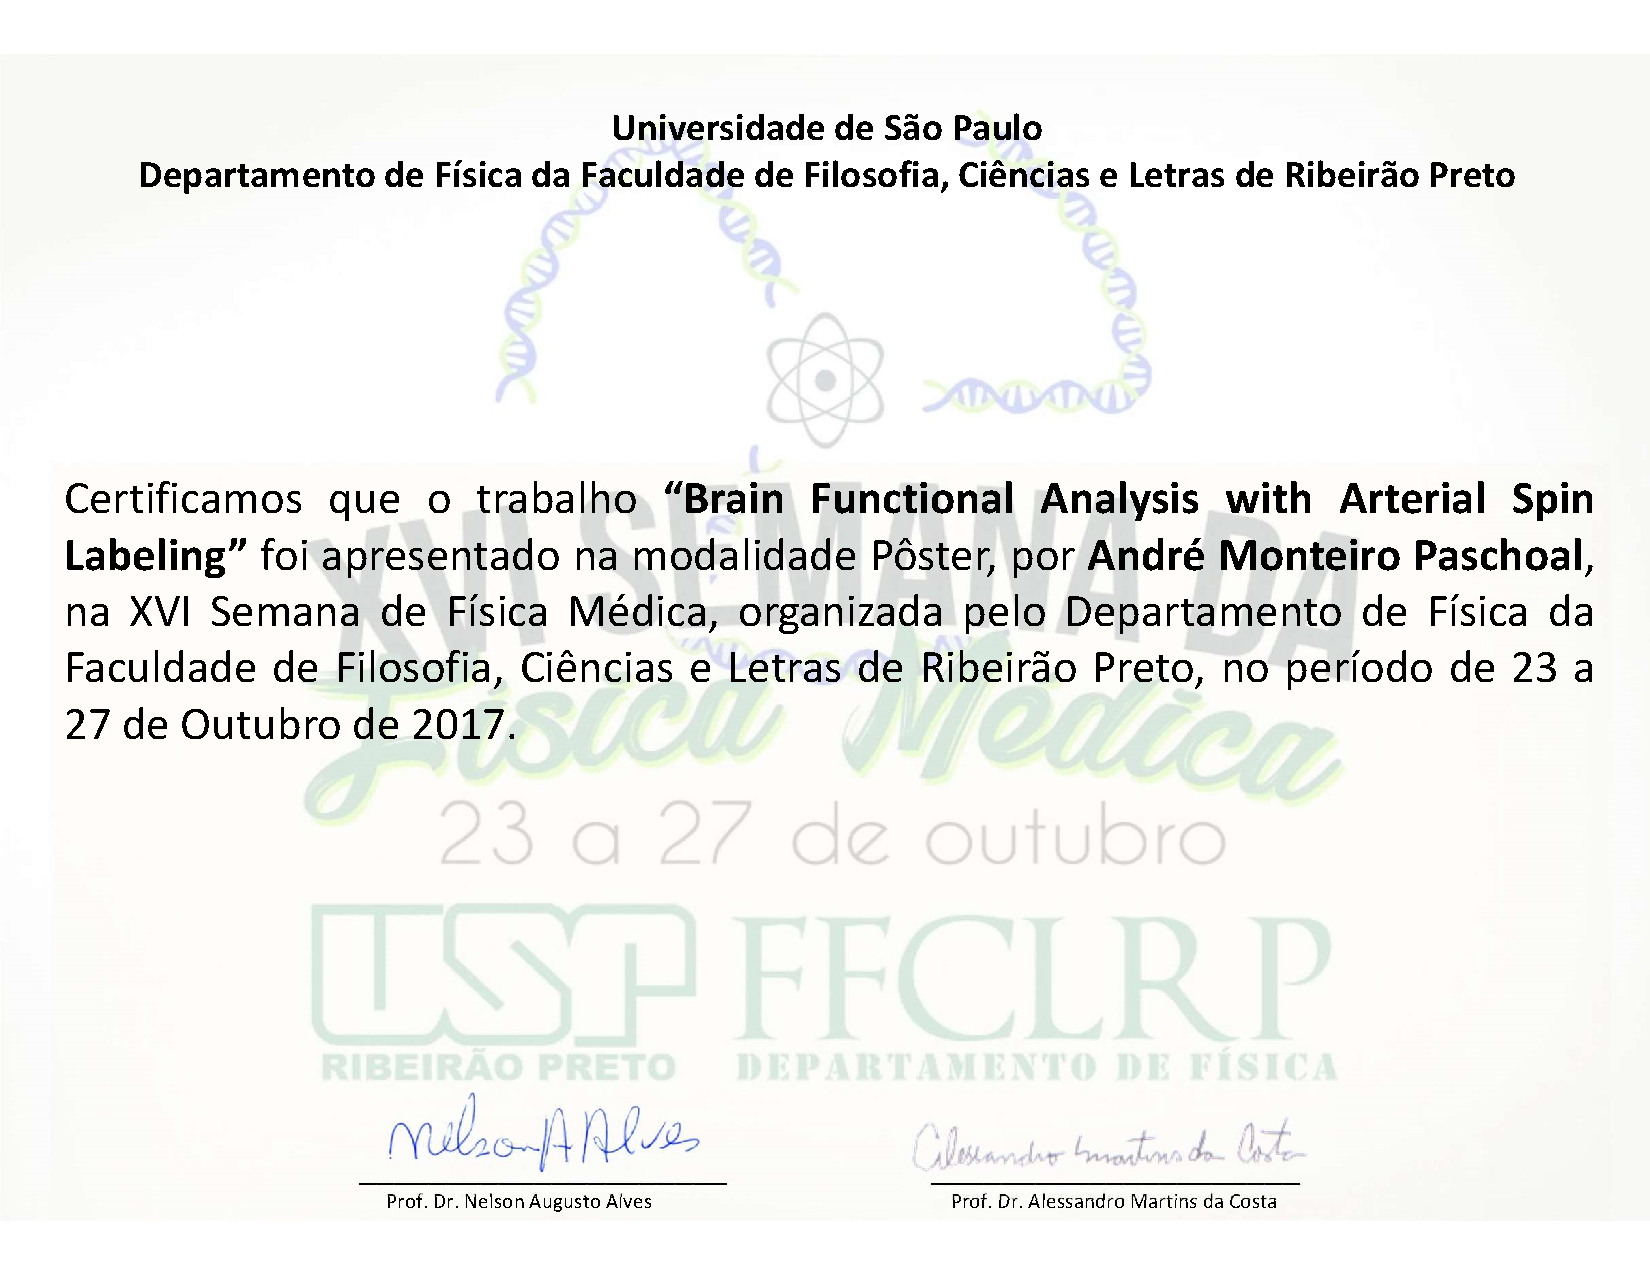
\includepdf[pages=-, scale=1,pagecommand=\thispagestyle{empty}]{\detokenize{Diplomas/SFM2017}}

\newpage
\subsection{Participa\c{c}\~{a}o em Eventos Cient\'{\i}ficos (com apresenta\c{c}\~{a}o de trabalho ou oferecimento de cursos, palestras ou debates}
\label{certificados:SFM2017_avaliador}
Esta subseção apresenta o comprovante da participação na XV Semana da Física Médica com seus respectivos propósitos.
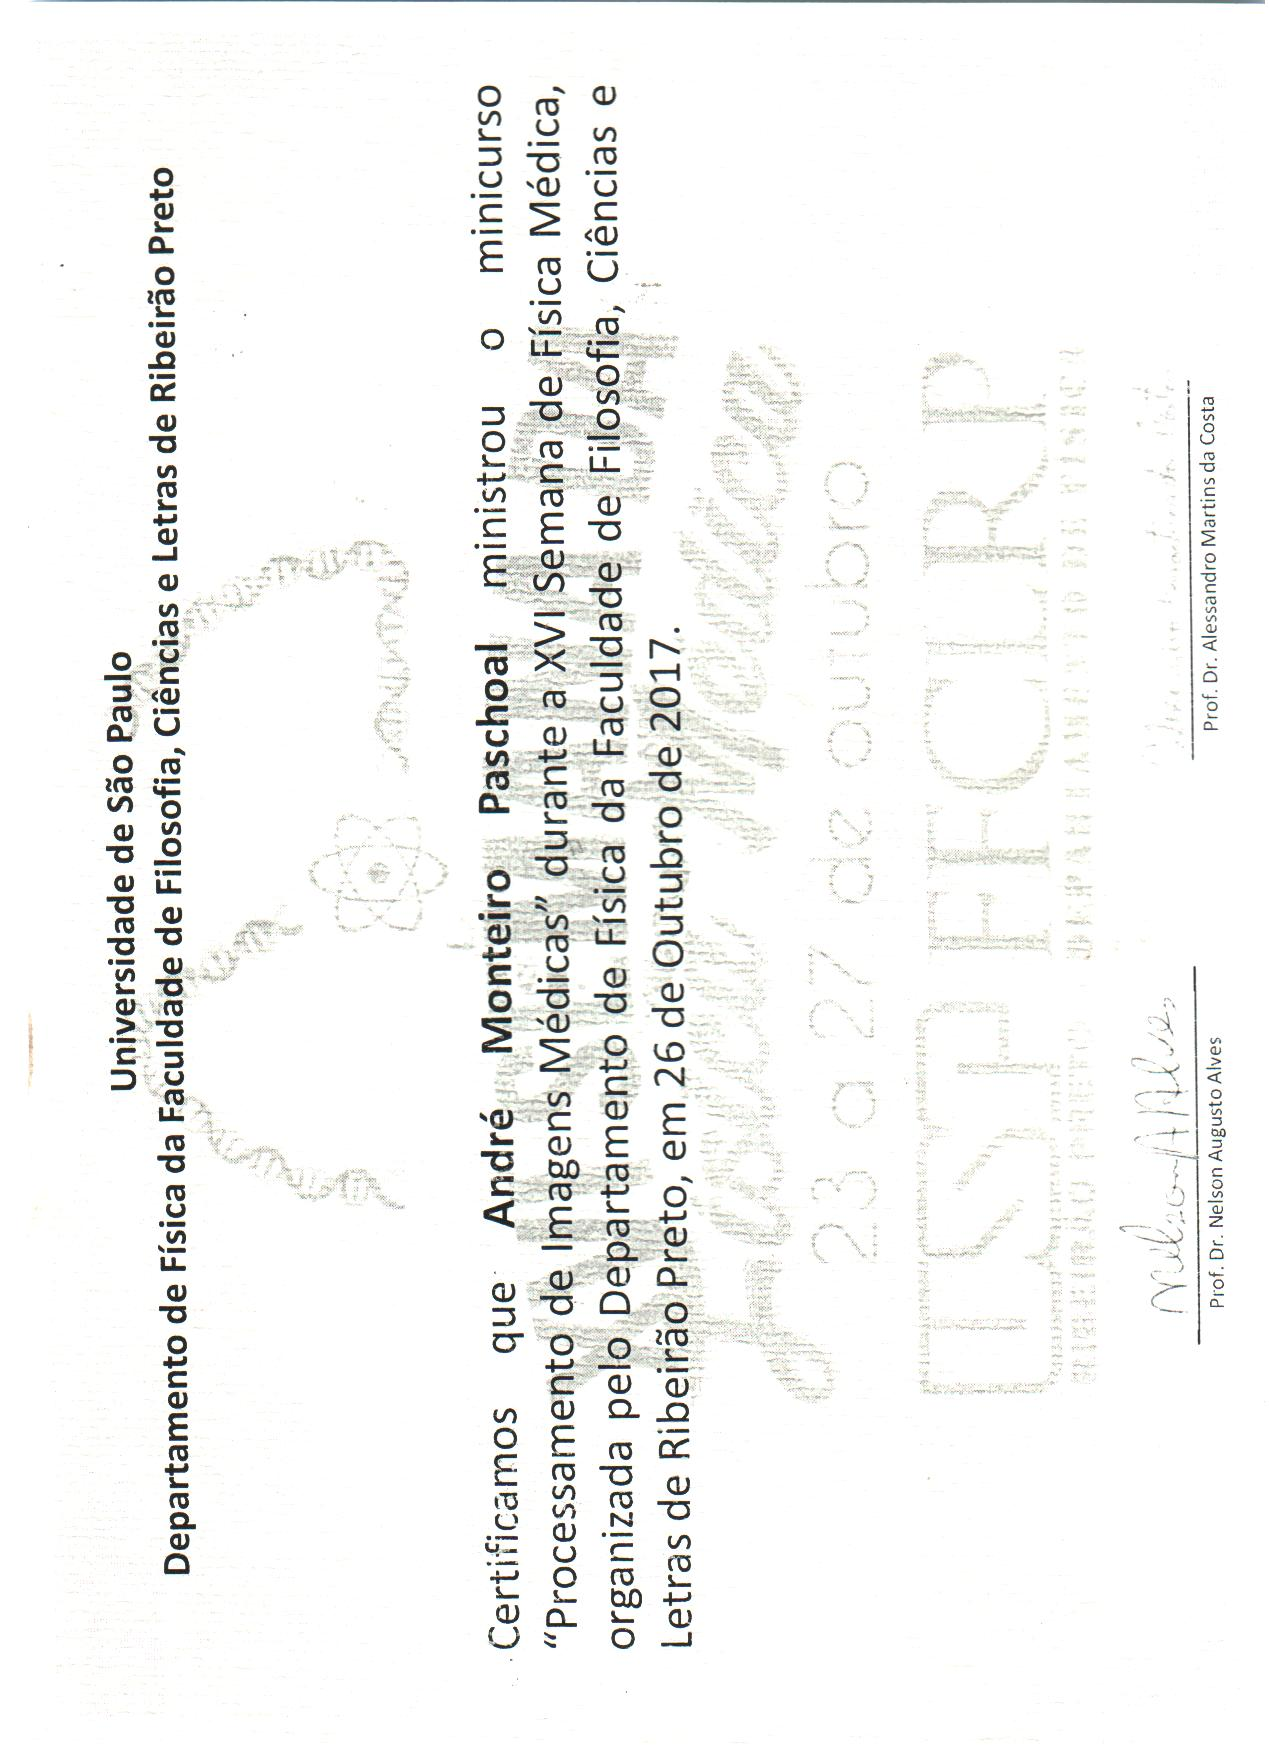
\includepdf[pages=-, scale=1,pagecommand=\thispagestyle{empty}]{\detokenize{Diplomas/CertificadoApresentacaoMiniCursoSFM}}

\newpage
\subsection{Participa\c{c}\~{a}o em Eventos Cient\'{\i}ficos (com apresenta\c{c}\~{a}o de trabalho ou oferecimento de cursos, palestras ou debates}
\label{certificados:SFM2018}
Esta subseção apresenta o comprovante da participação na XV Semana da Física Médica com seus respectivos propósitos.
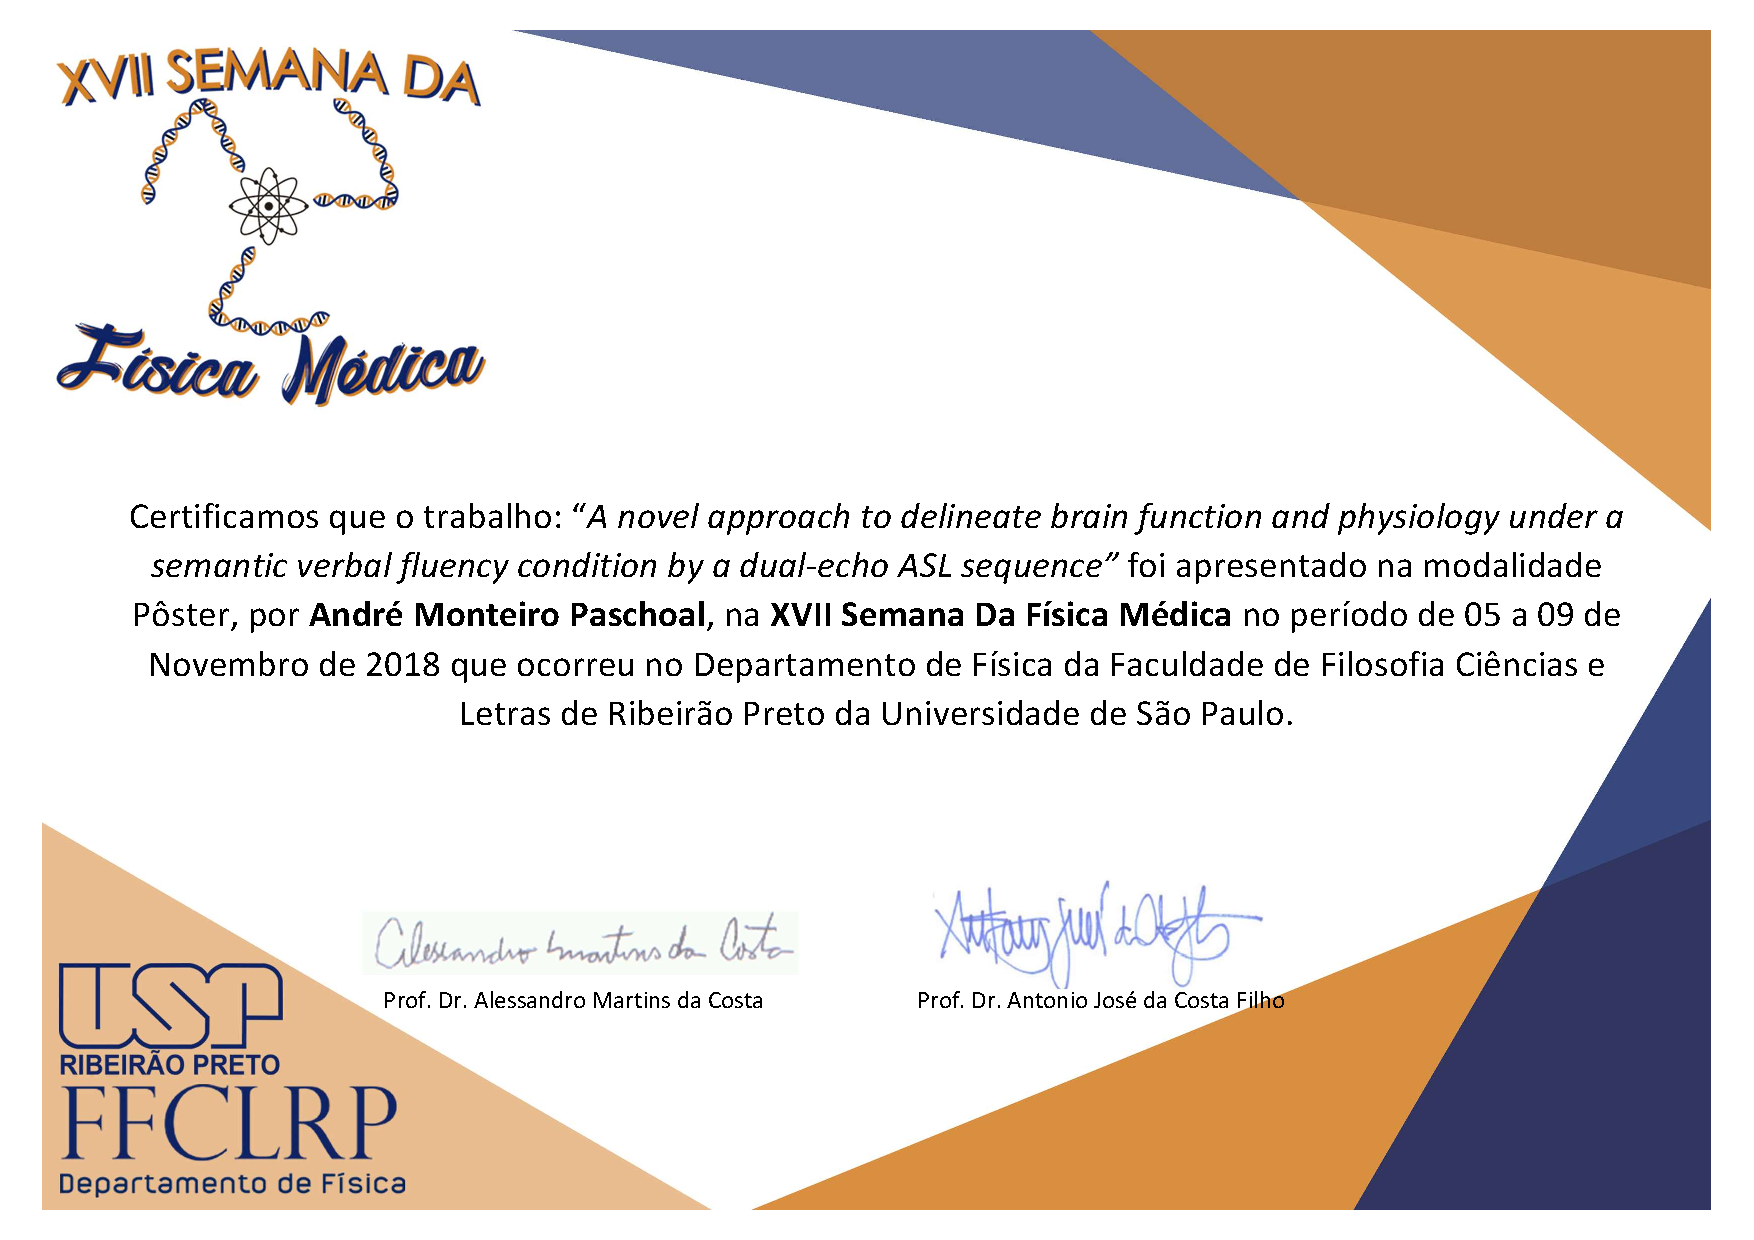
\includepdf[pages=-, scale=1,pagecommand=\thispagestyle{empty}]{\detokenize{Diplomas/SFM2018}}

\newpage
\subsection{Participa\c{c}\~{a}o em Eventos Cient\'{\i}ficos (com apresenta\c{c}\~{a}o de trabalho ou oferecimento de cursos, palestras ou debates}
\label{certificados:ISMRMBenelux}
Esta subseção apresenta o comprovante da participação no ISMRM Benelux Chapter com seus respectivos propósitos.

\includepdf[pages=-, scale=1,pagecommand=\thispagestyle{empty}]{\detokenize{Diplomas/certificate-ISMRMBenelux2019-Andre}}

\newpage
\subsection{Participa\c{c}\~{a}o em Eventos Cient\'{\i}ficos (com apresenta\c{c}\~{a}o de trabalho ou oferecimento de cursos, palestras ou debates}
\label{certificados:OHBM2019}
Esta subseção apresenta o comprovante da participação no Organization for Human Brain Mapping Annual Meeting com seus respectivos propósitos. \\
Obs: Ese congresso não emite certificado de apresentação de trabalhos, apenas de participação no evento.
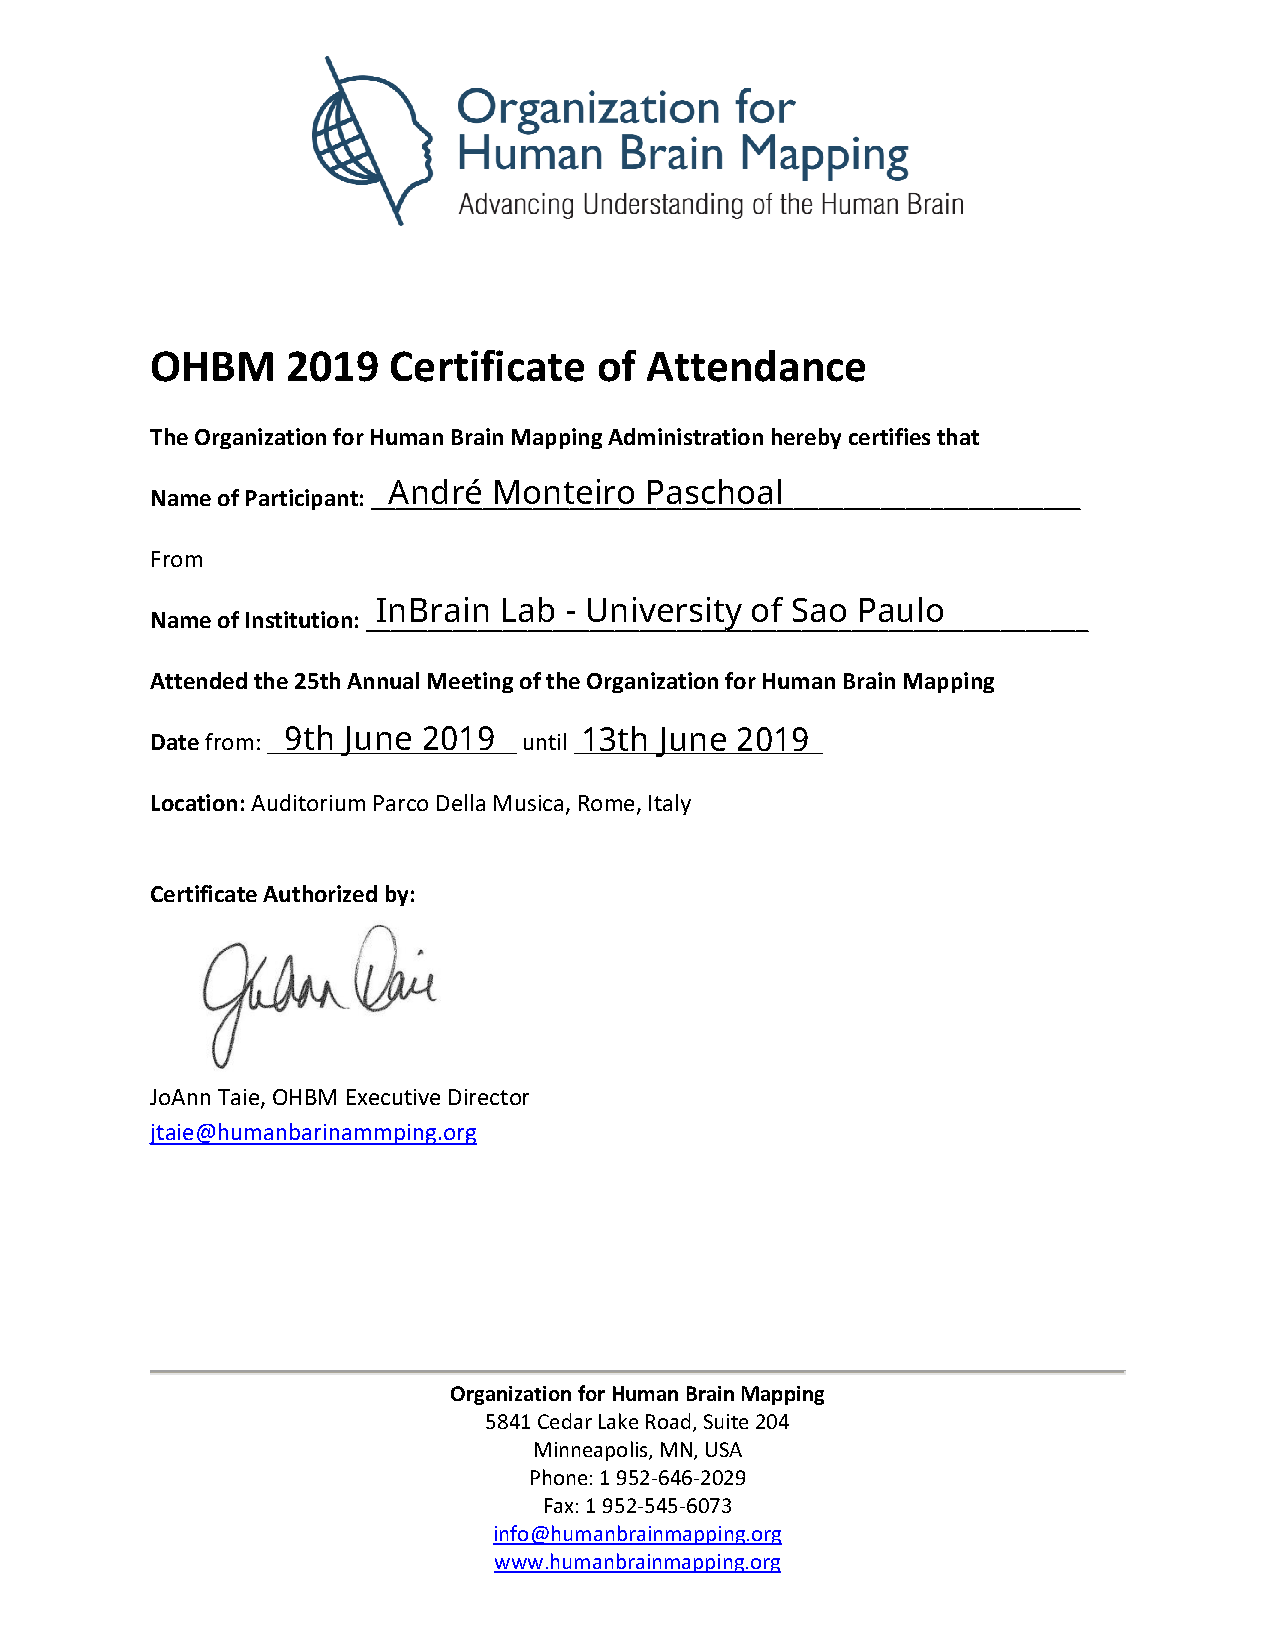
\includepdf[pages=-, scale=1,pagecommand=\thispagestyle{empty}]{\detokenize{Diplomas/Certificate of Attendance_OHBM-editado}}
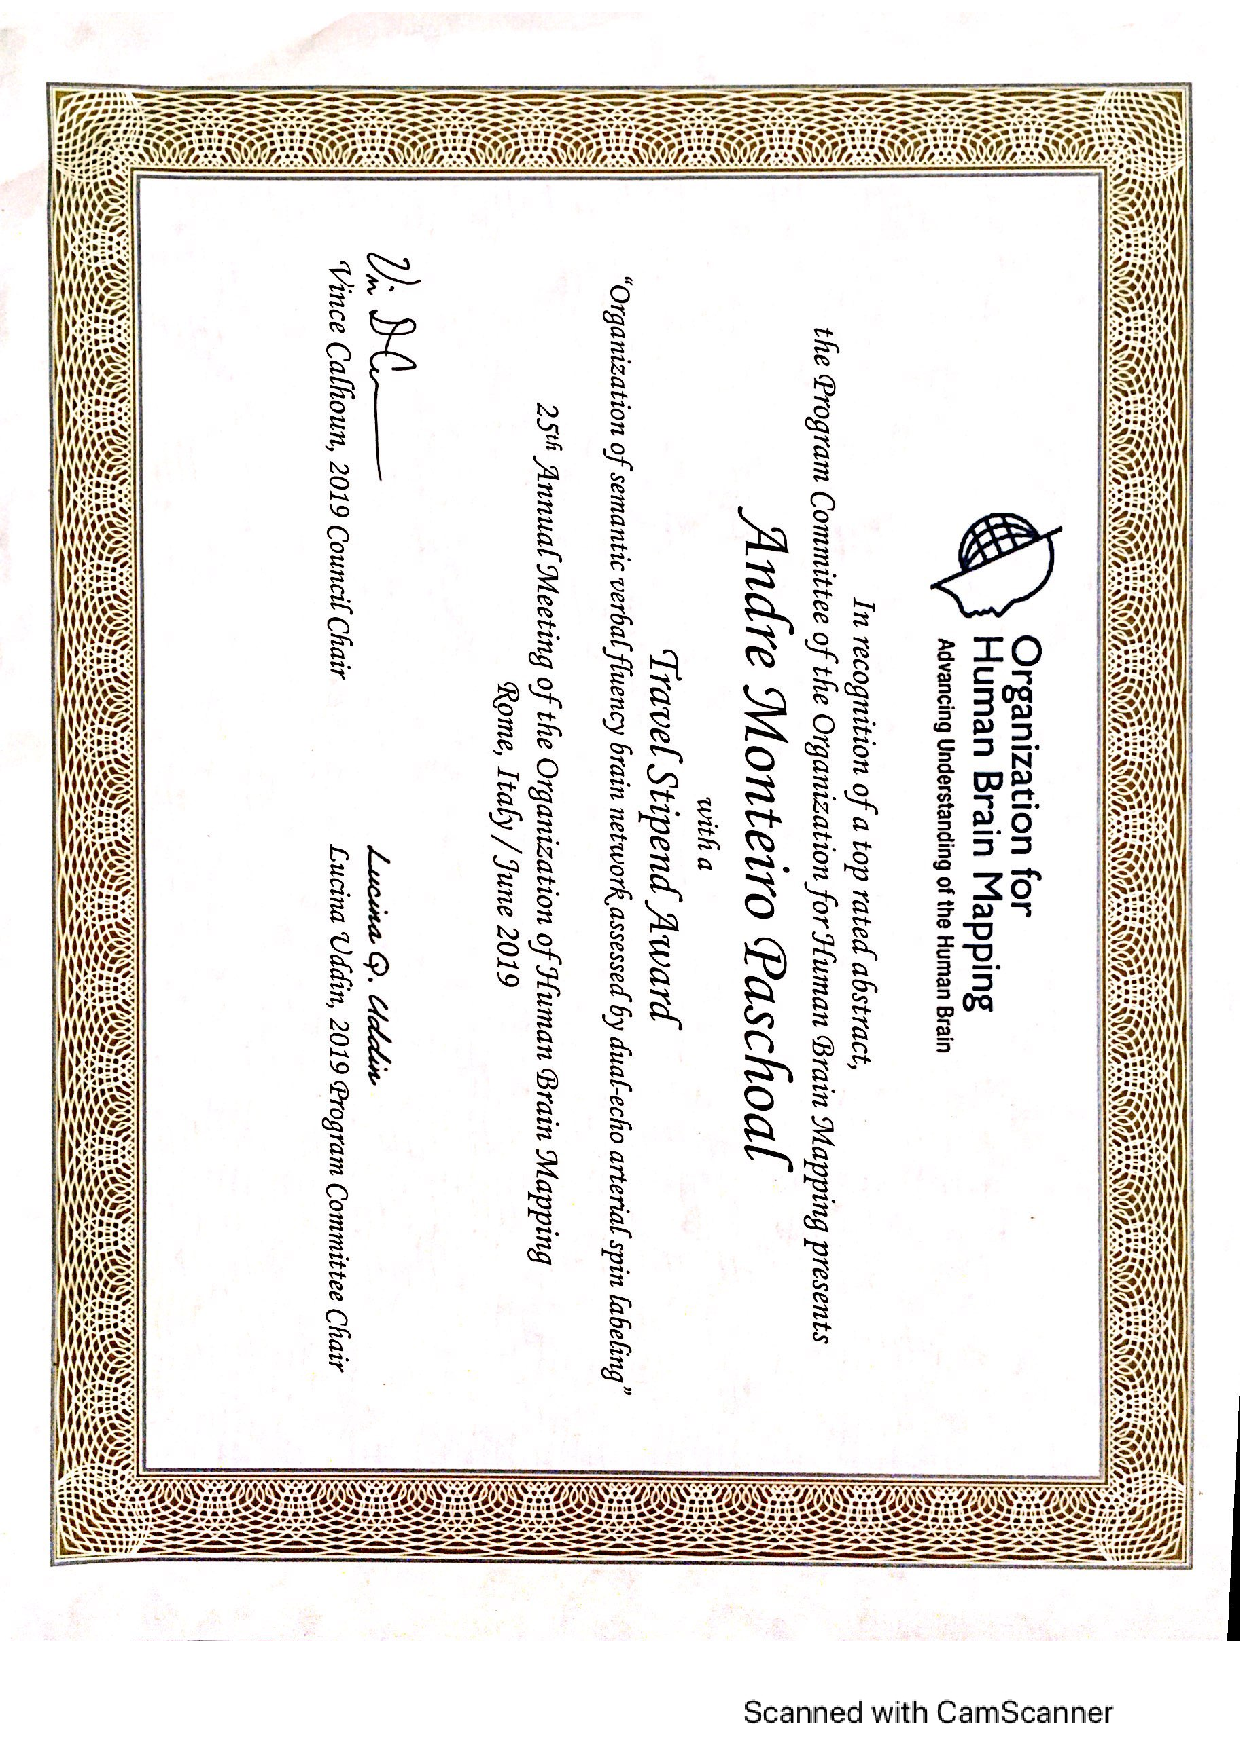
\includepdf[pages=-, scale=1,pagecommand=\thispagestyle{empty}]{\detokenize{Diplomas/OHBMtravelAward}}
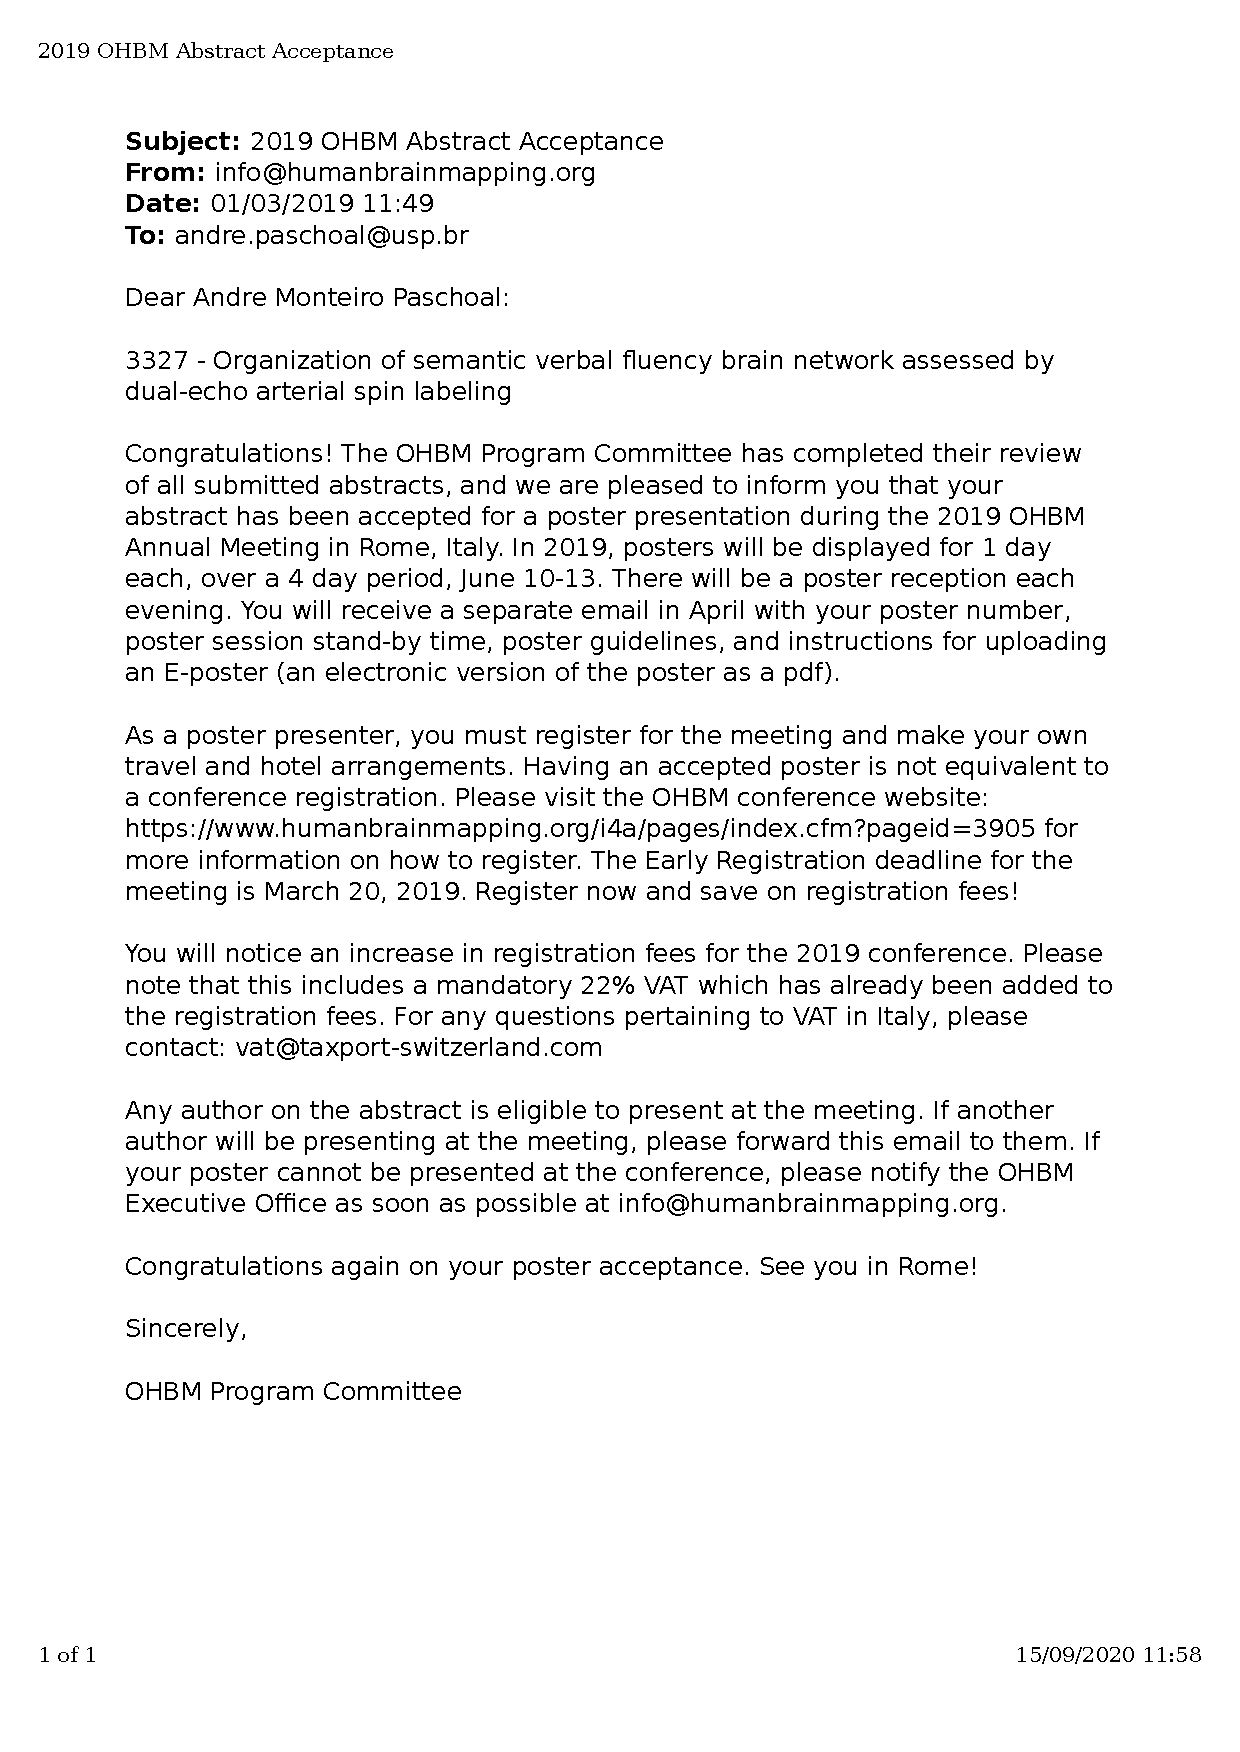
\includepdf[pages=-, scale=1,pagecommand=\thispagestyle{empty}]{\detokenize{Diplomas/AcceptanceOHBM2019}}

\newpage
\subsection{Participa\c{c}\~{a}o em Eventos Cient\'{\i}ficos (com apresenta\c{c}\~{a}o de trabalho ou oferecimento de cursos, palestras ou debates}
\label{certificados:SFM2019}
Esta subseção apresenta o comprovante da participação na XV Semana da Física Médica com seus respectivos propósitos.
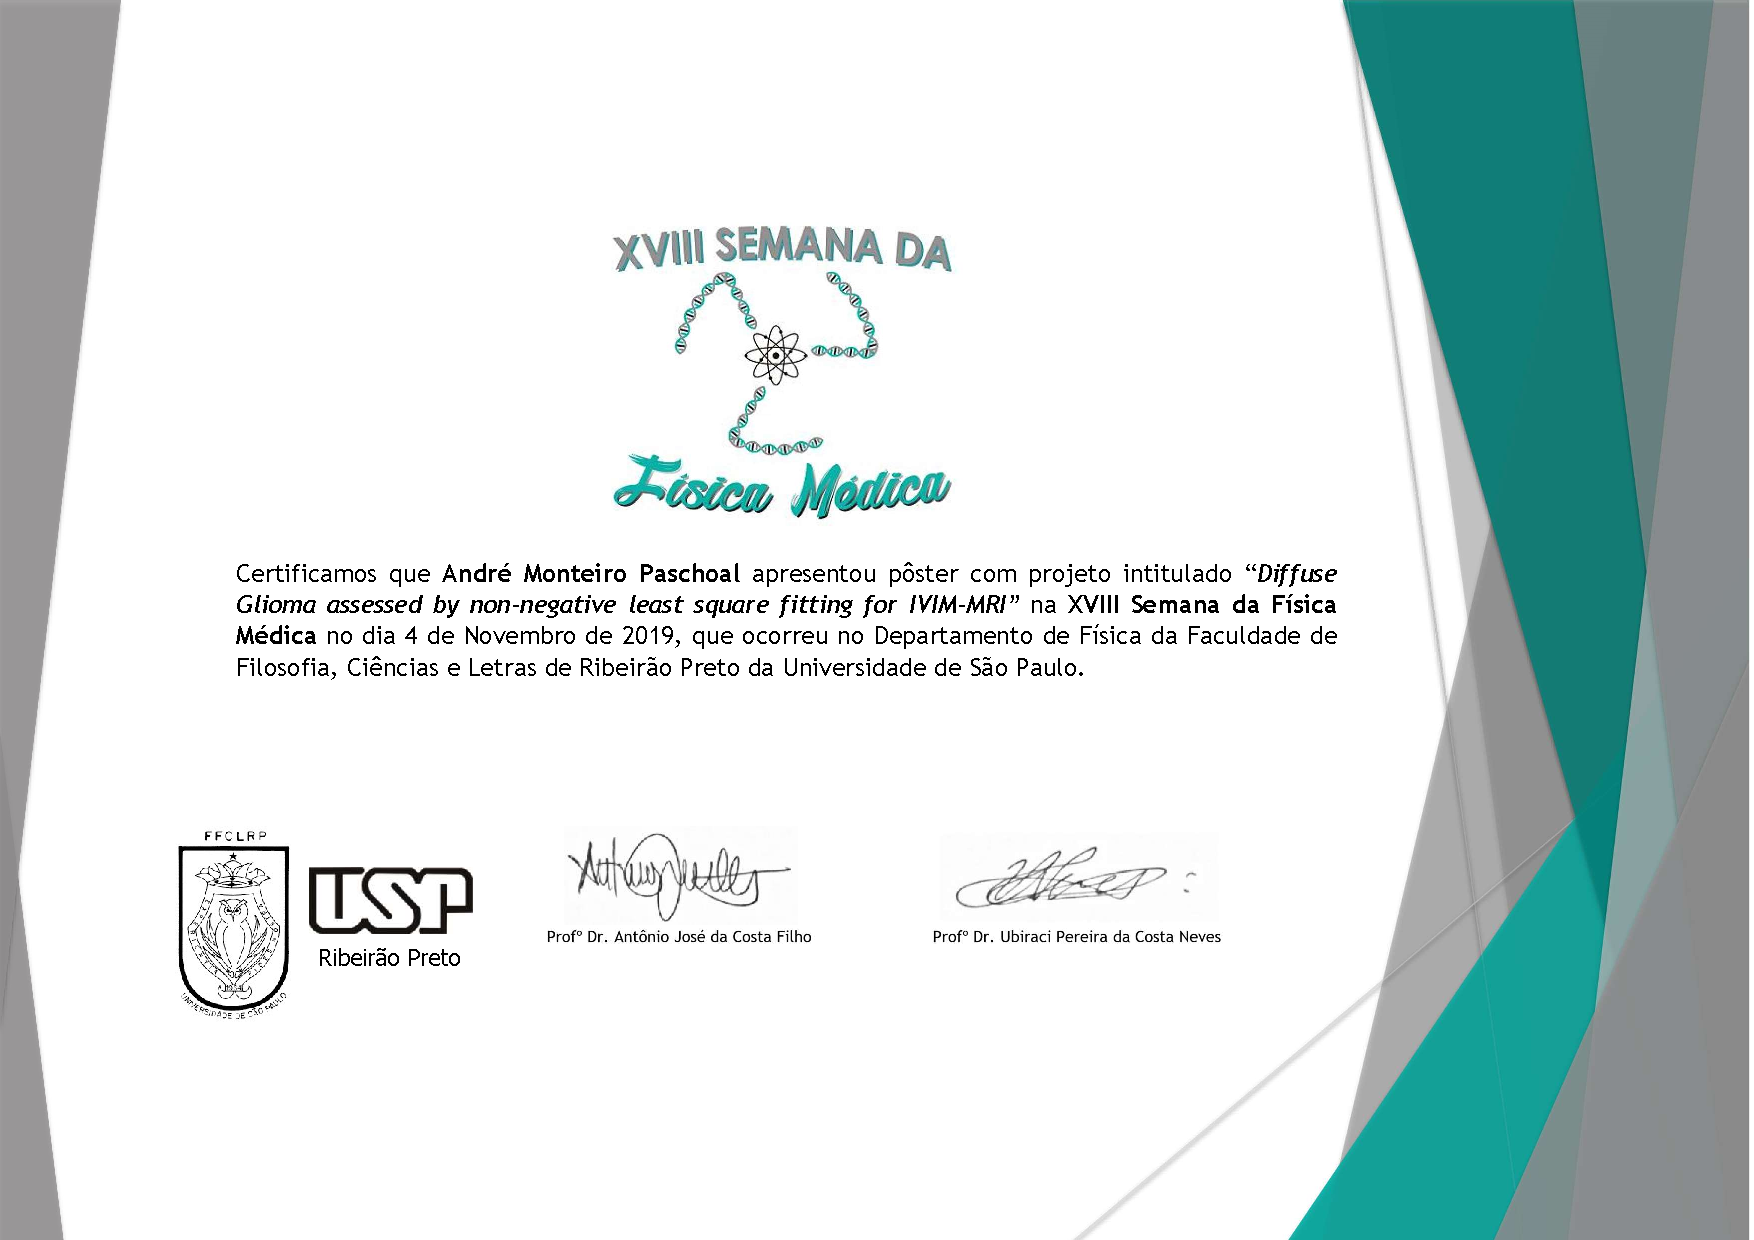
\includepdf[pages=-, scale=1,pagecommand=\thispagestyle{empty}]{\detokenize{Diplomas/SFM2019}}

\newpage
\subsection{Participa\c{c}\~{a}o em Eventos Cient\'{\i}ficos (com apresenta\c{c}\~{a}o de trabalho ou oferecimento de cursos, palestras ou debates}
\label{certificados:mrtrix3}
Esta subseção apresenta o comprovante da participação no 3rd MRTrix 3 Workshop com seus respectivos propósitos.
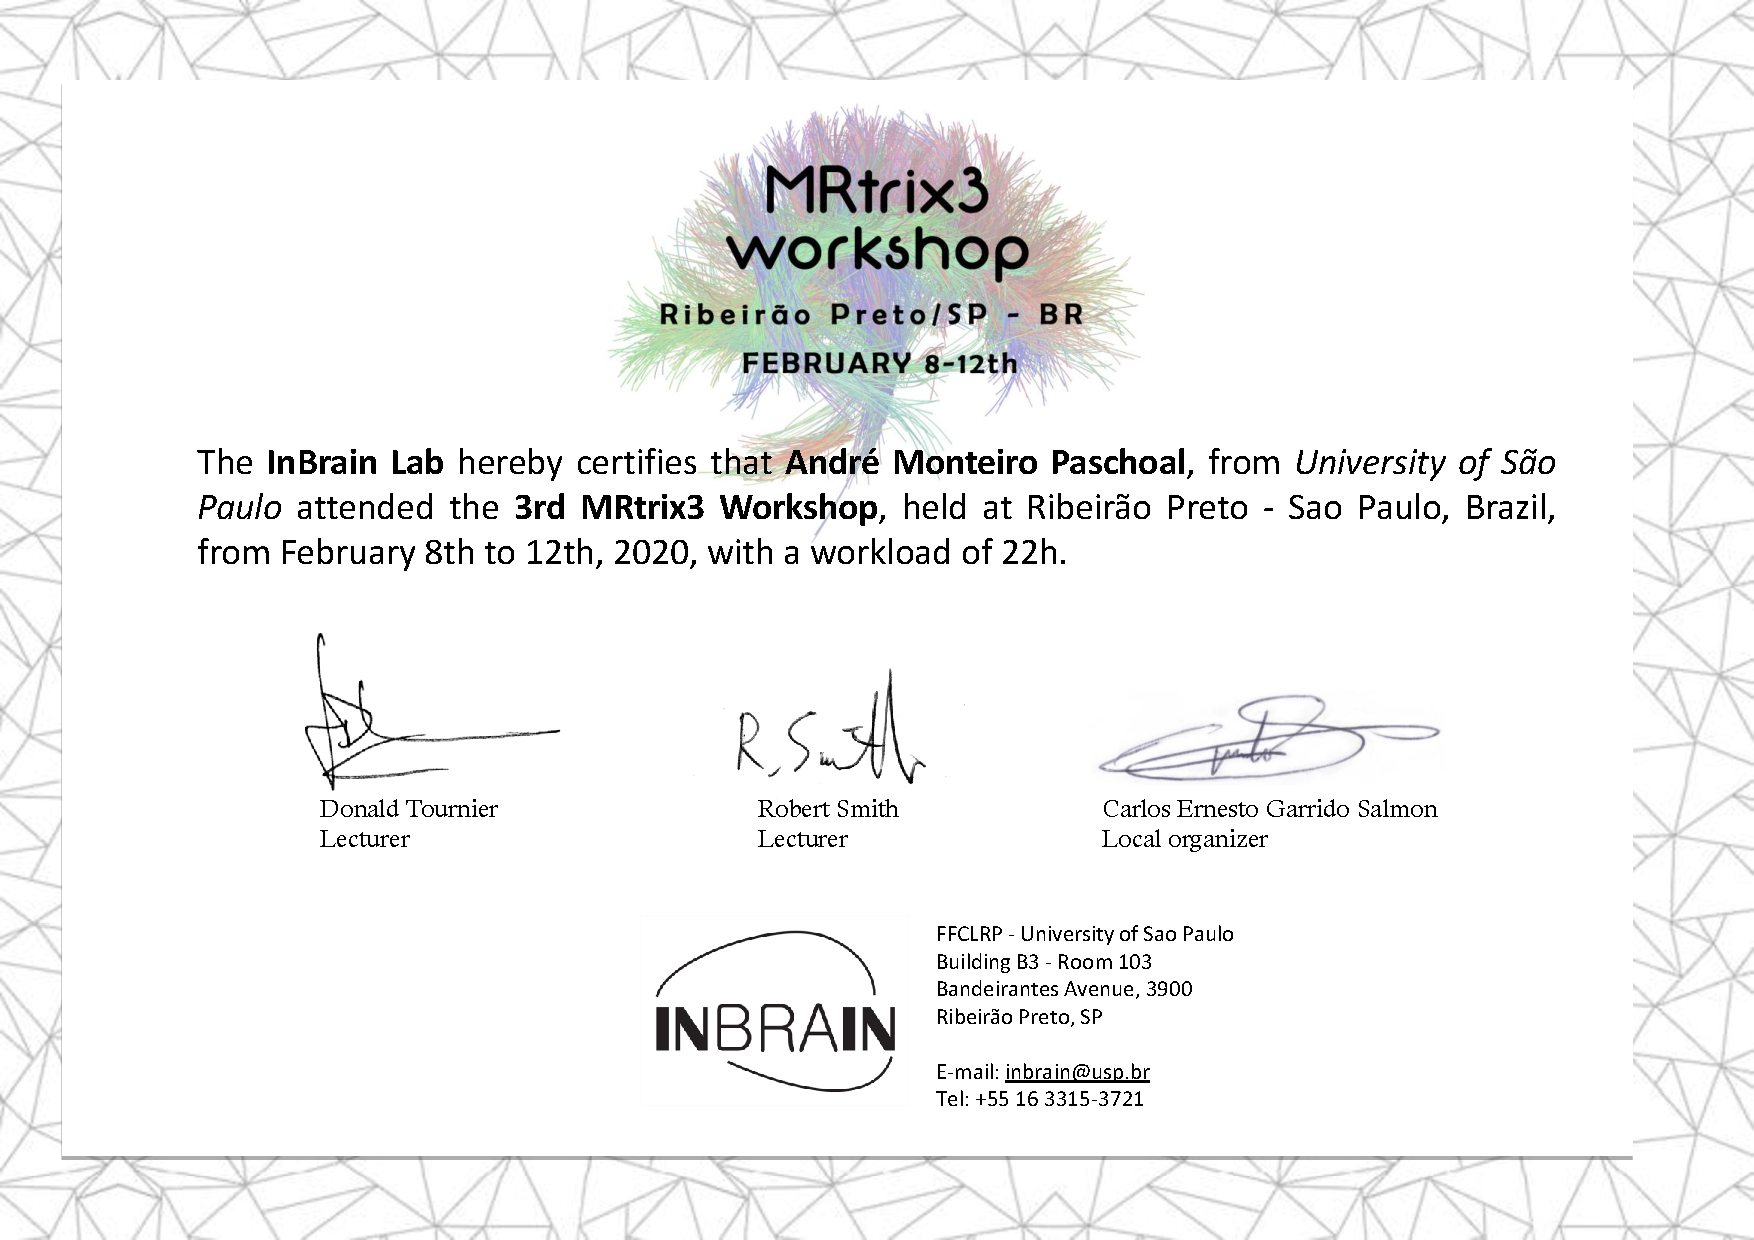
\includepdf[pages=-, scale=1,pagecommand=\thispagestyle{empty}]{\detokenize{Diplomas/mrtrix3workshop}}

\newpage
\subsection{Participa\c{c}\~{a}o em Eventos Cient\'{\i}ficos (com apresenta\c{c}\~{a}o de trabalho ou oferecimento de cursos, palestras ou debates}
\label{certificados:inbrain2020}
Esta subseção apresenta o comprovante da participação no InBrain Workshop 2020: Advanced Brain Imaging com seus respectivos propósitos.
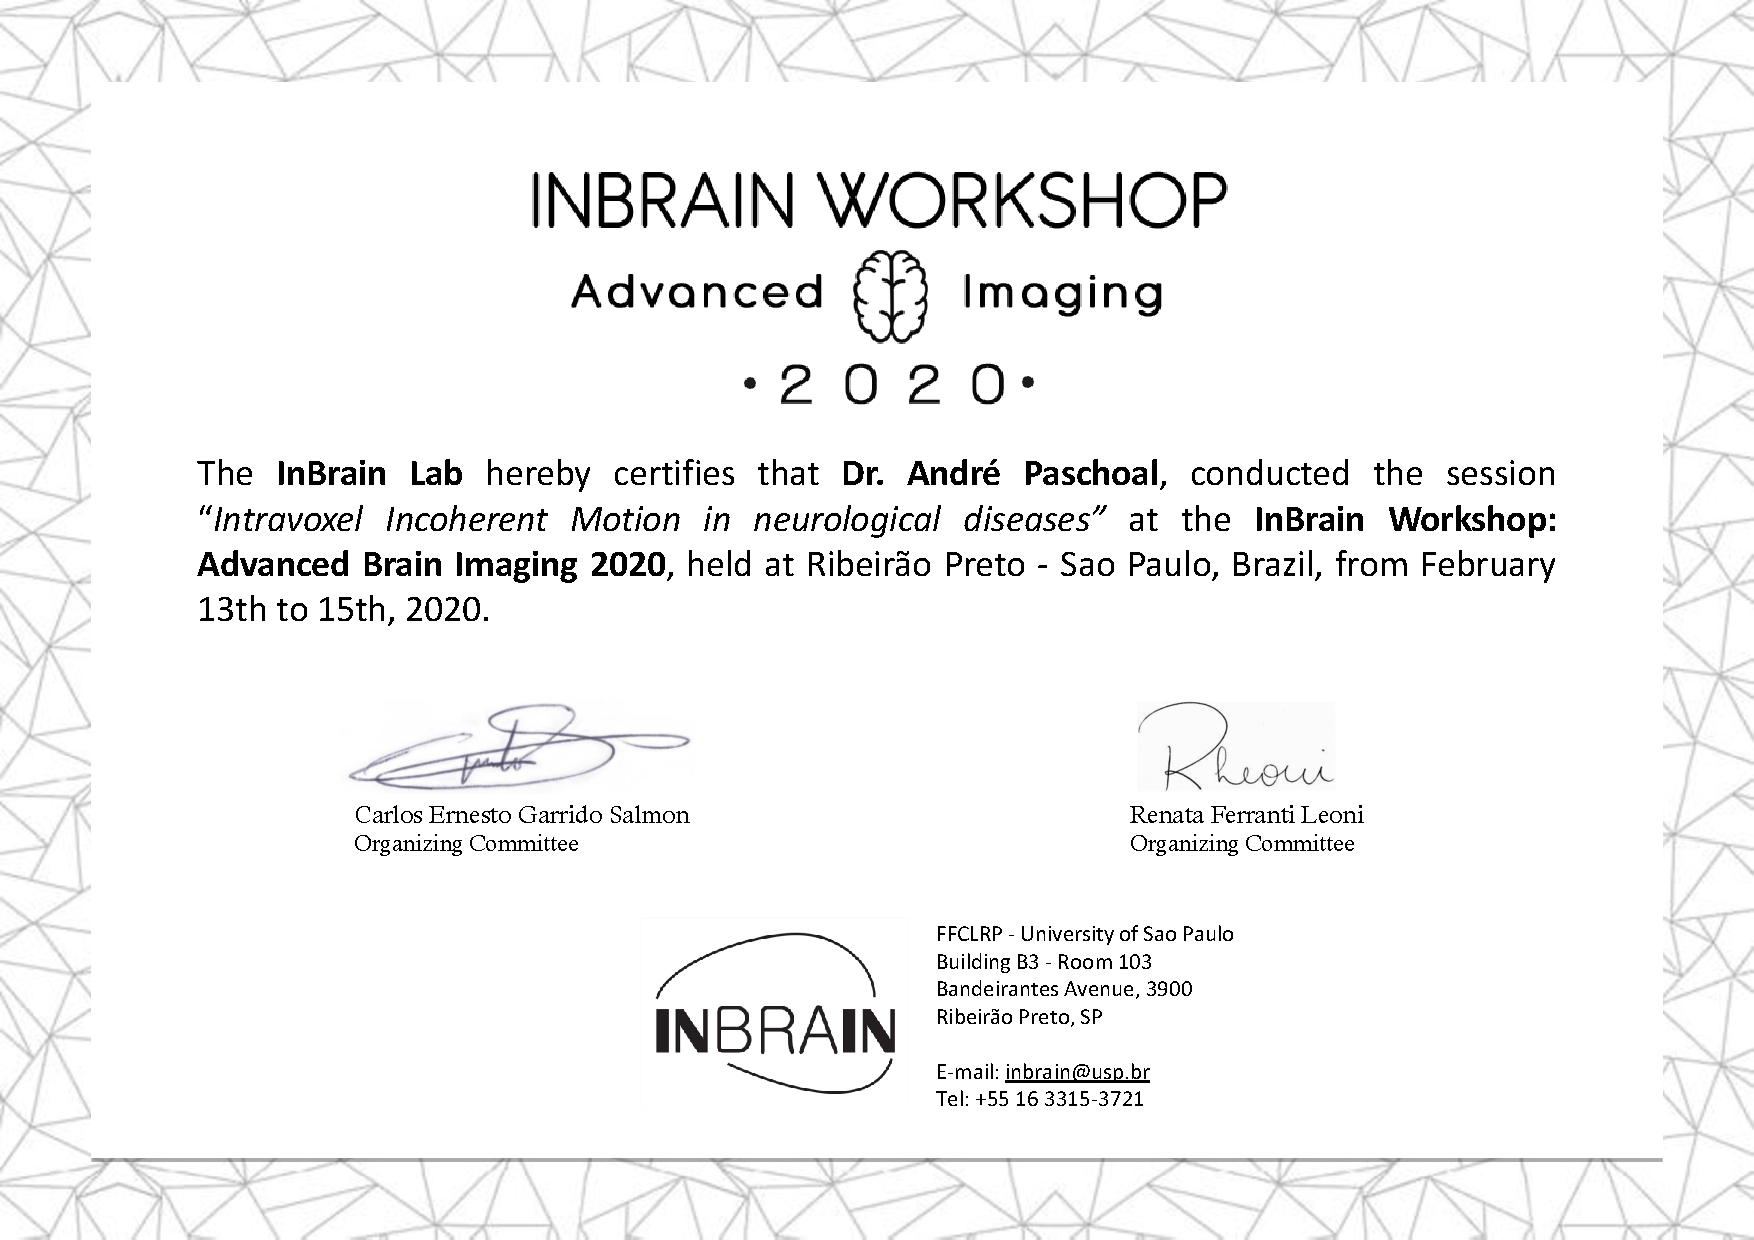
\includepdf[pages=-, scale=1,pagecommand=\thispagestyle{empty}]{\detokenize{Diplomas/InBrainWorkshop_palestrante}}

\newpage
\subsection{Participa\c{c}\~{a}o em Eventos Cient\'{\i}ficos (com apresenta\c{c}\~{a}o de trabalho ou oferecimento de cursos, palestras ou debates}
\label{certificados:ISMRM2020}
Esta subseção apresenta o comprovante da participação no 
ISMRM 28th Annual Meeting \& Exhibition com seus respectivos propósitos. \\
%Obs: Ese congresso não emite certificado de apresentação de trabalhos, apenas de participação no evento.
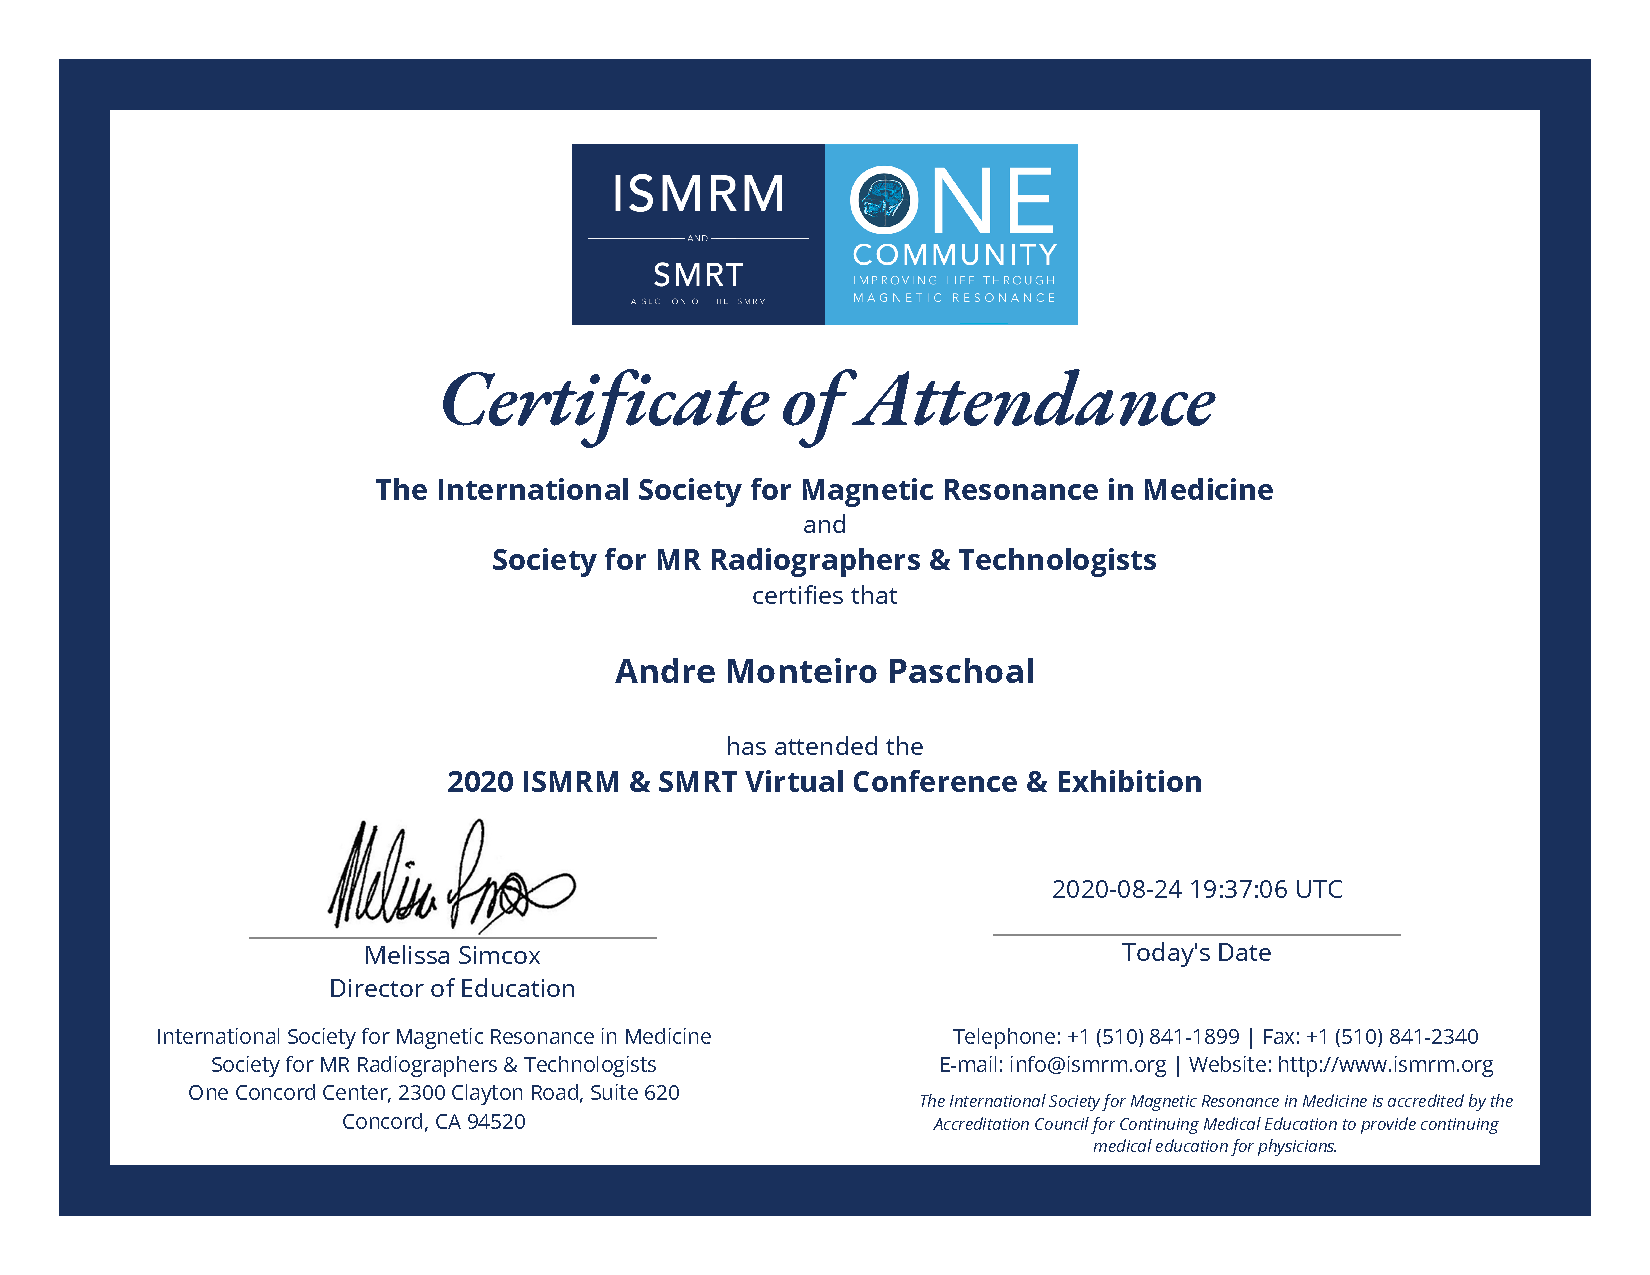
\includepdf[pages=-, scale=1,pagecommand=\thispagestyle{empty}]{\detokenize{Diplomas/ISMRM2020}}
%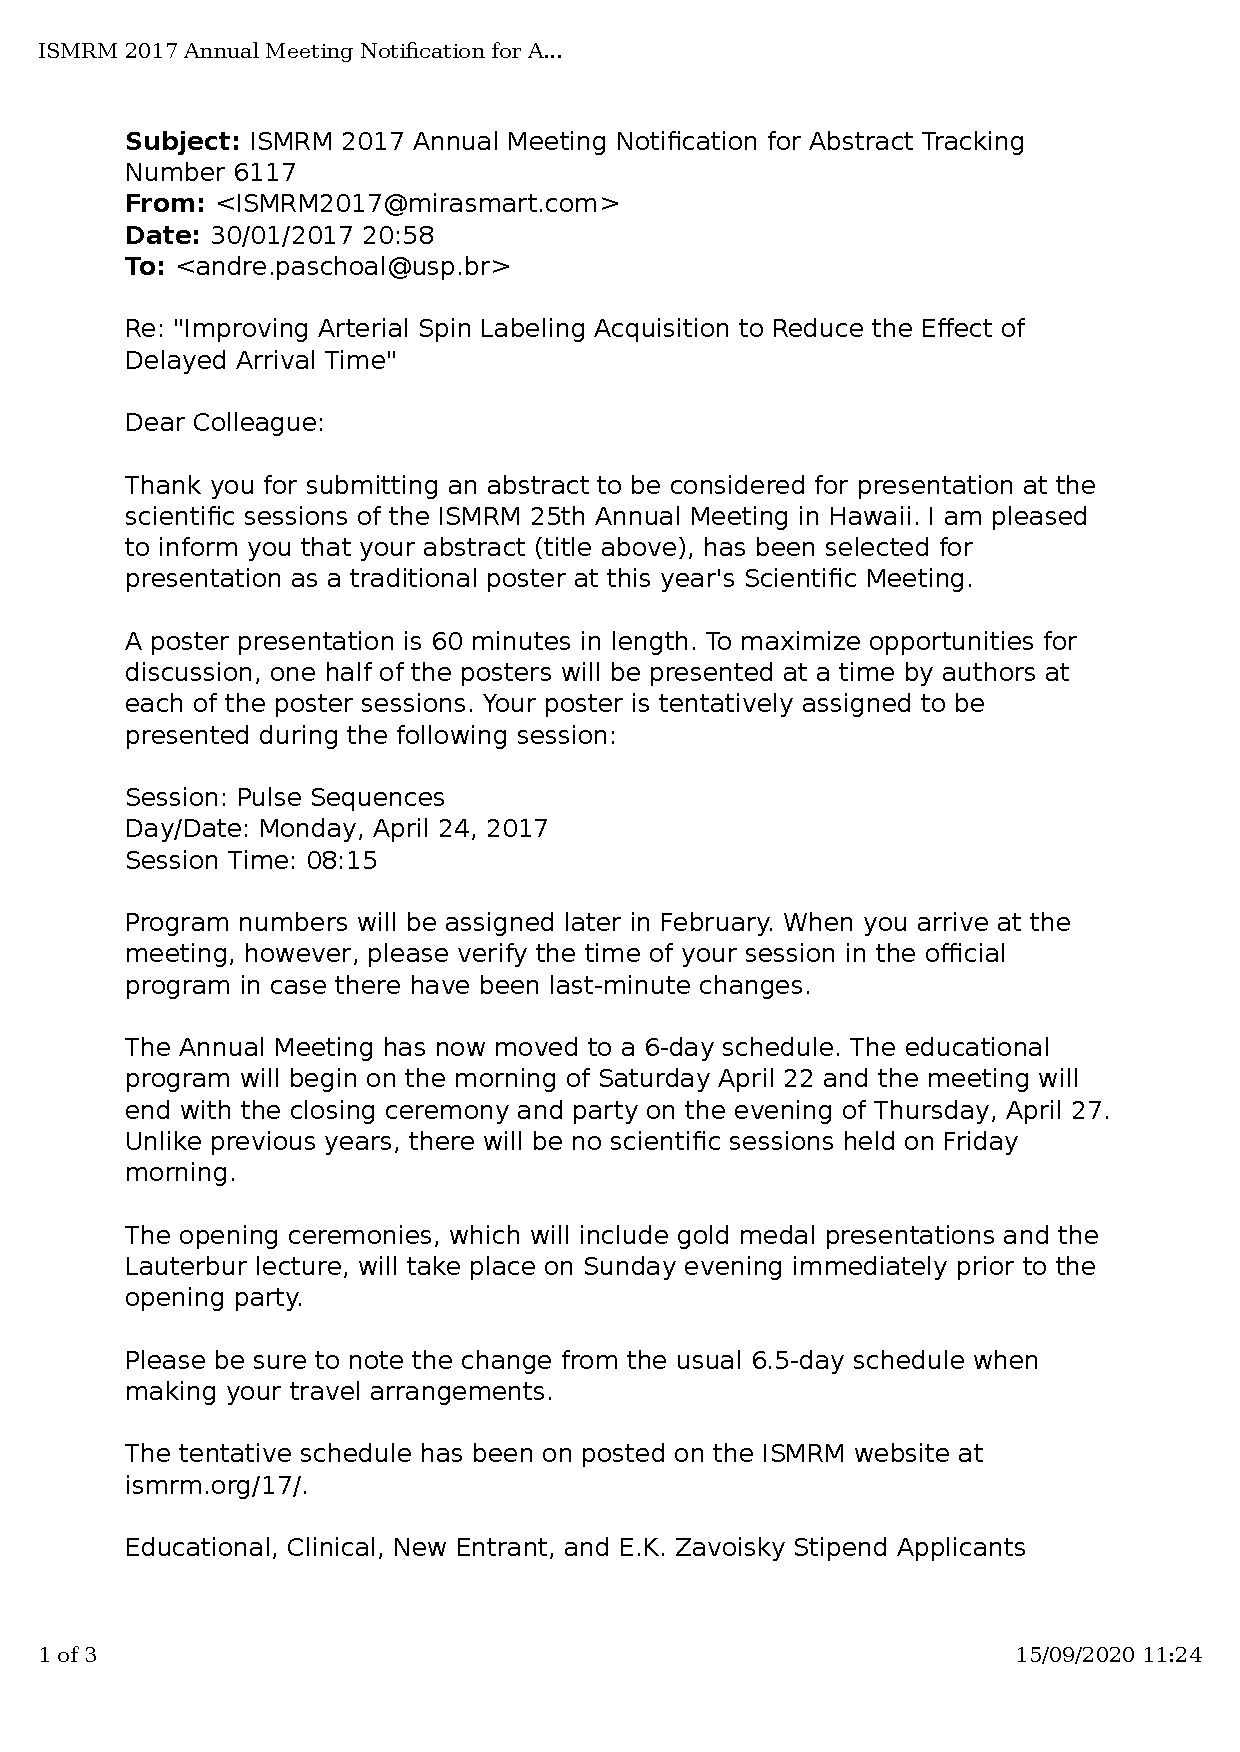
\includepdf[pages=-, scale=1,pagecommand=\thispagestyle{empty}]{\detokenize{Diplomas/AcceptanceISMRM2017}}

\newpage
\subsection{Participa\c{c}\~{a}o em Eventos Cient\'{\i}ficos (com apresenta\c{c}\~{a}o de trabalho ou oferecimento de cursos, palestras ou debates}
\label{certificados:ESMRMB2020}
Esta subseção apresenta o comprovante da participação no 
ESMRMB 37th Annual Meeting \& Exhibition com seus respectivos propósitos. \\
Obs: Ese congresso não emite certificado de apresentação de trabalhos, apenas de participação no evento.
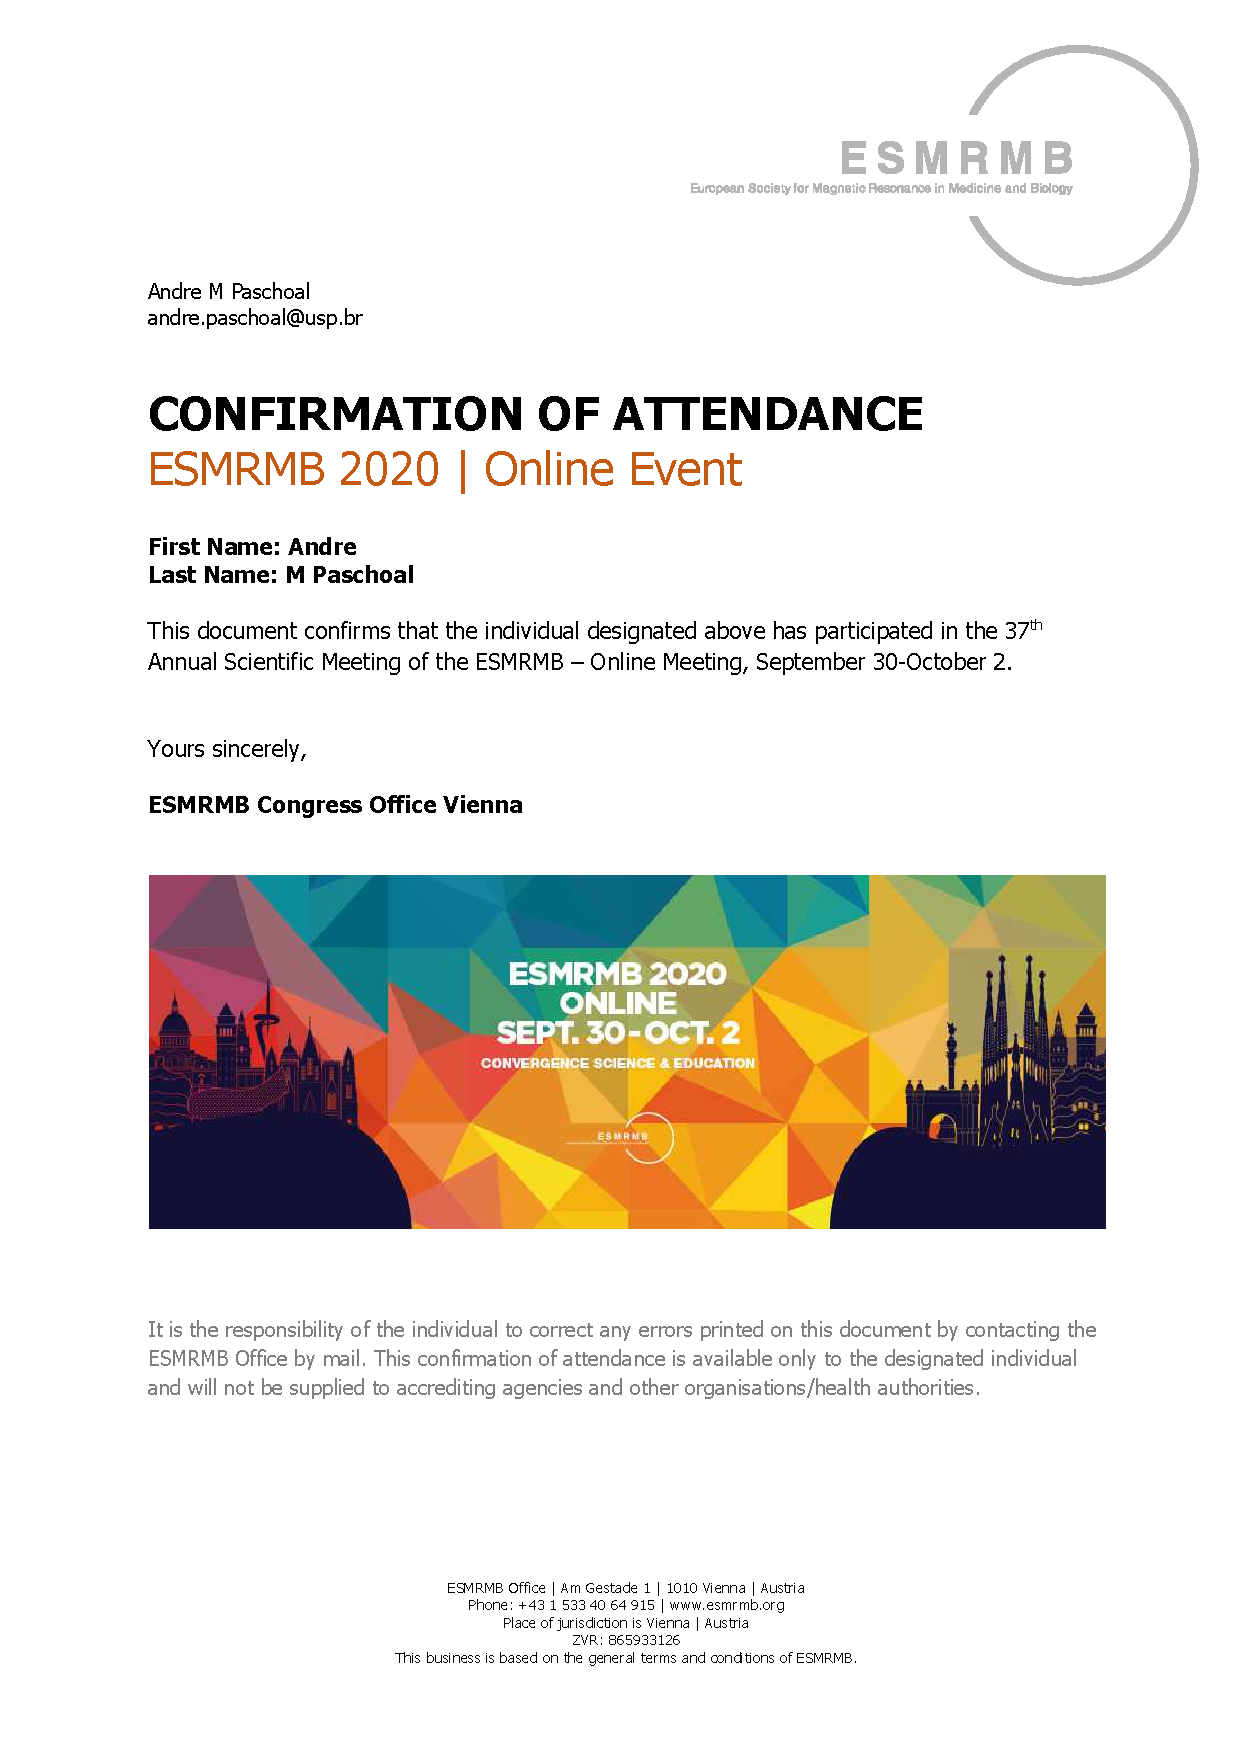
\includepdf[pages=-, scale=1,pagecommand=\thispagestyle{empty}]{\detokenize{Diplomas/ESMRMB2020}}
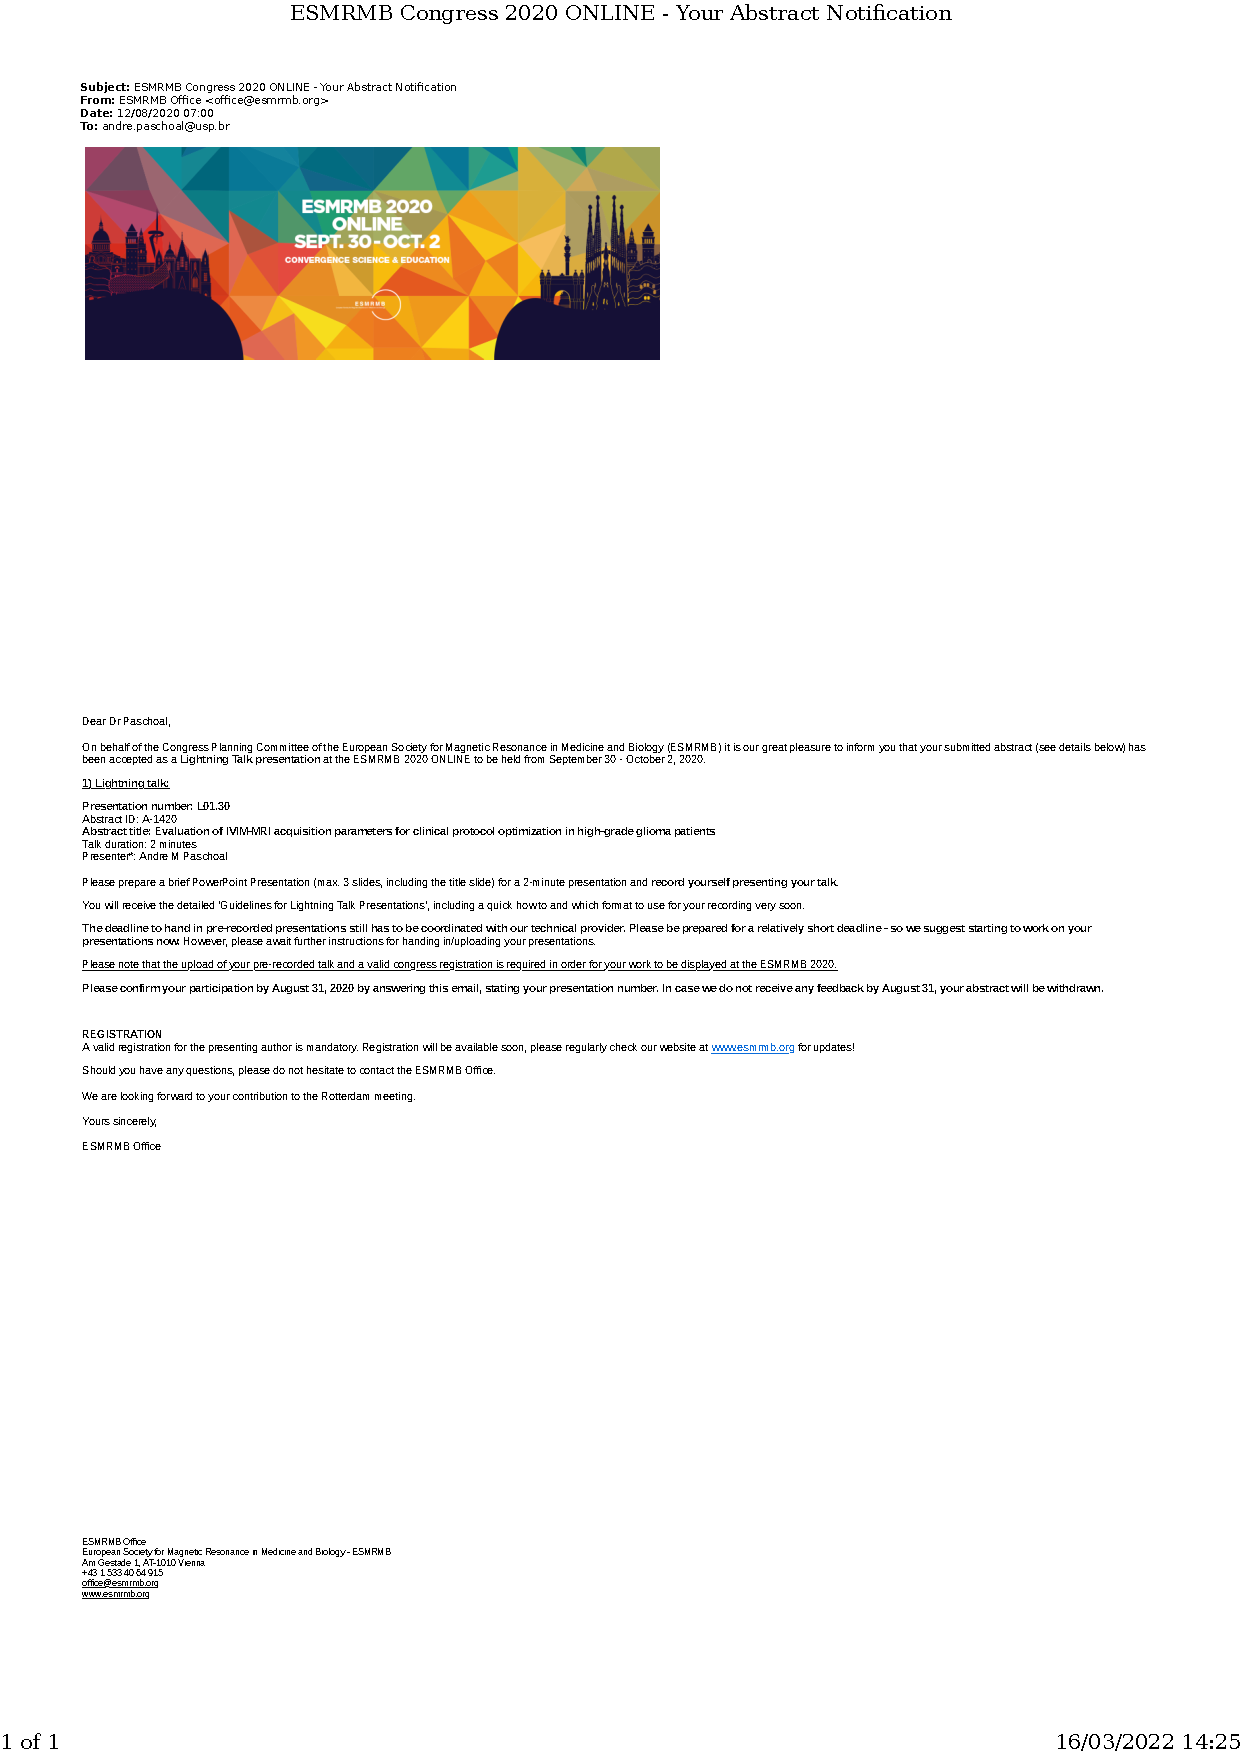
\includepdf[pages=-, scale=1,pagecommand=\thispagestyle{empty}]{\detokenize{Diplomas/AcceptanceESMRMB2020}}

\newpage
\subsection{Participa\c{c}\~{a}o em Eventos Cient\'{\i}ficos (com apresenta\c{c}\~{a}o de trabalho ou oferecimento de cursos, palestras ou debates}
\label{certificados:ISMRM2021}
Esta subseção apresenta o comprovante da participação no 
ISMRM 29th Annual Meeting \& Exhibition com seus respectivos propósitos. \\
Obs: Ese congresso não emite certificado de apresentação de trabalhos, apenas de participação no evento.
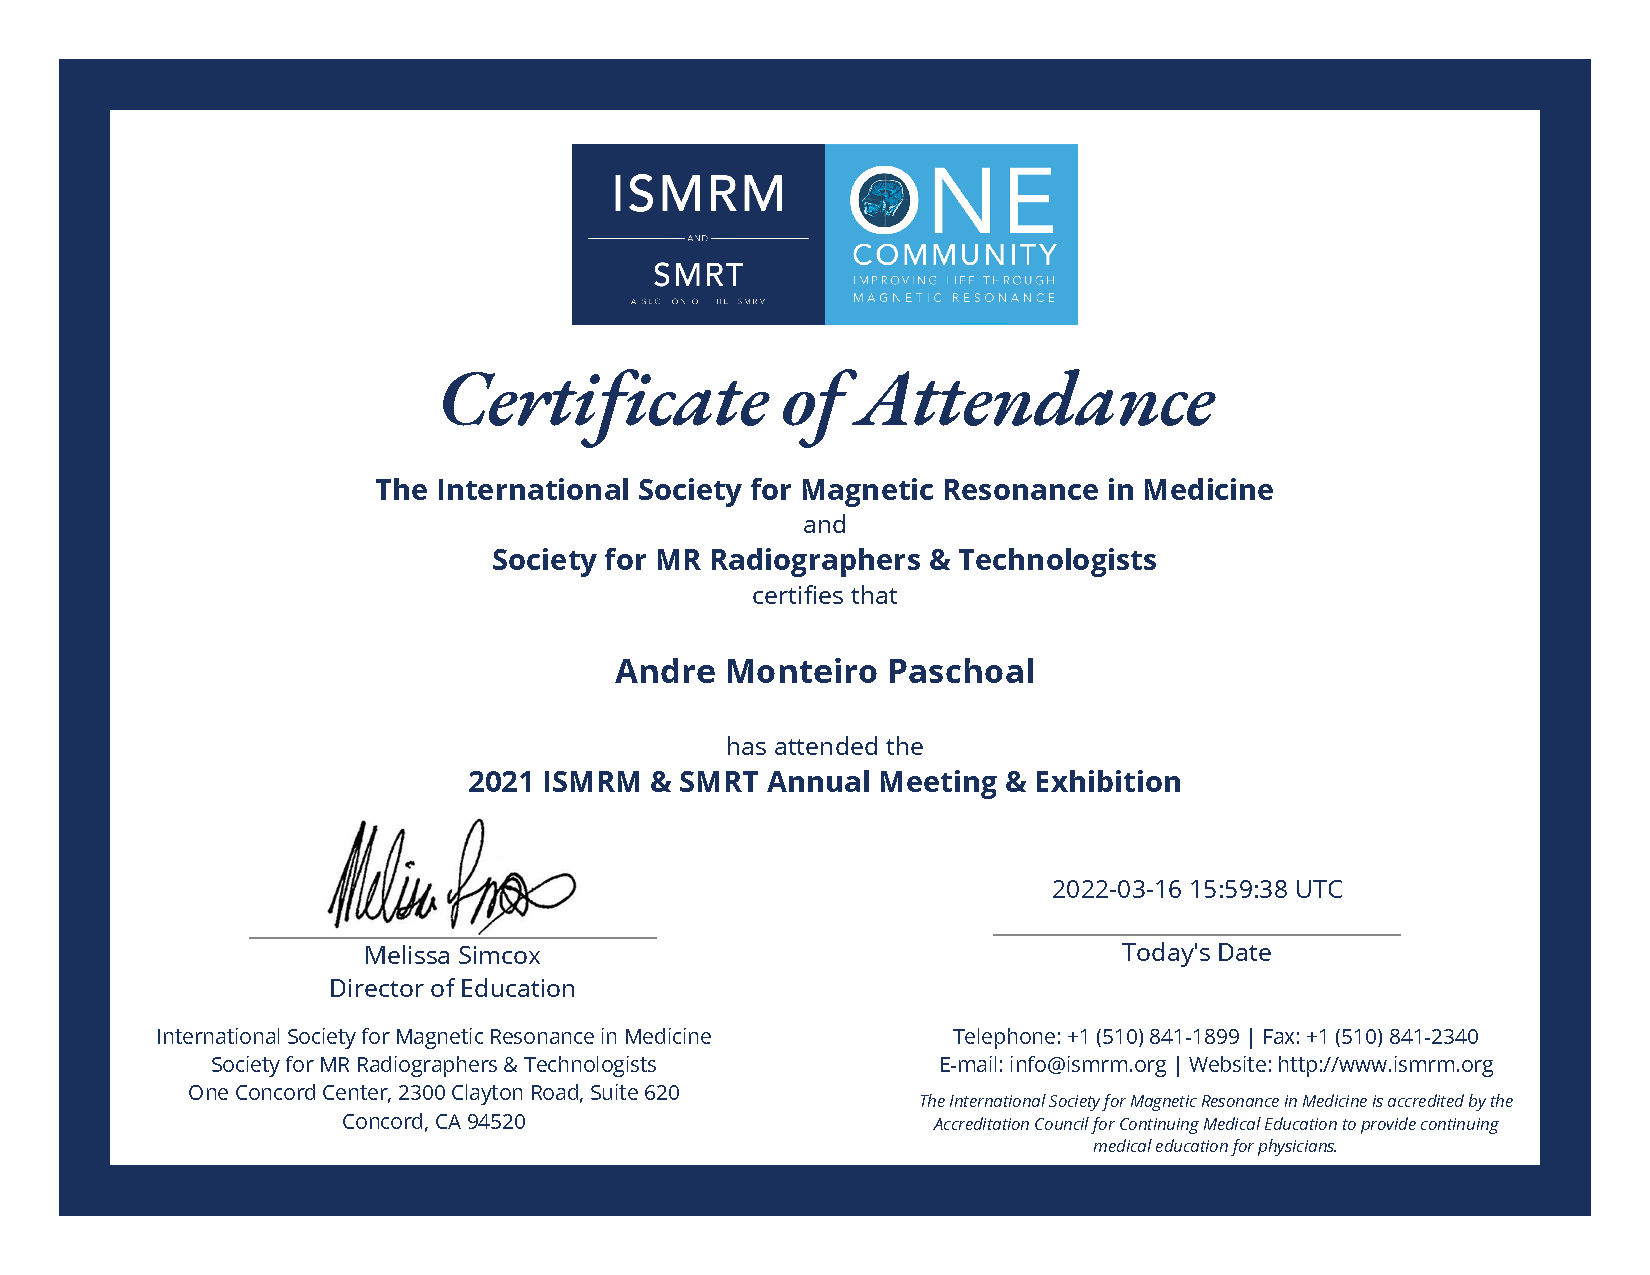
\includepdf[pages=-, scale=1,pagecommand=\thispagestyle{empty}]{\detokenize{Diplomas/ISMRM2021}}
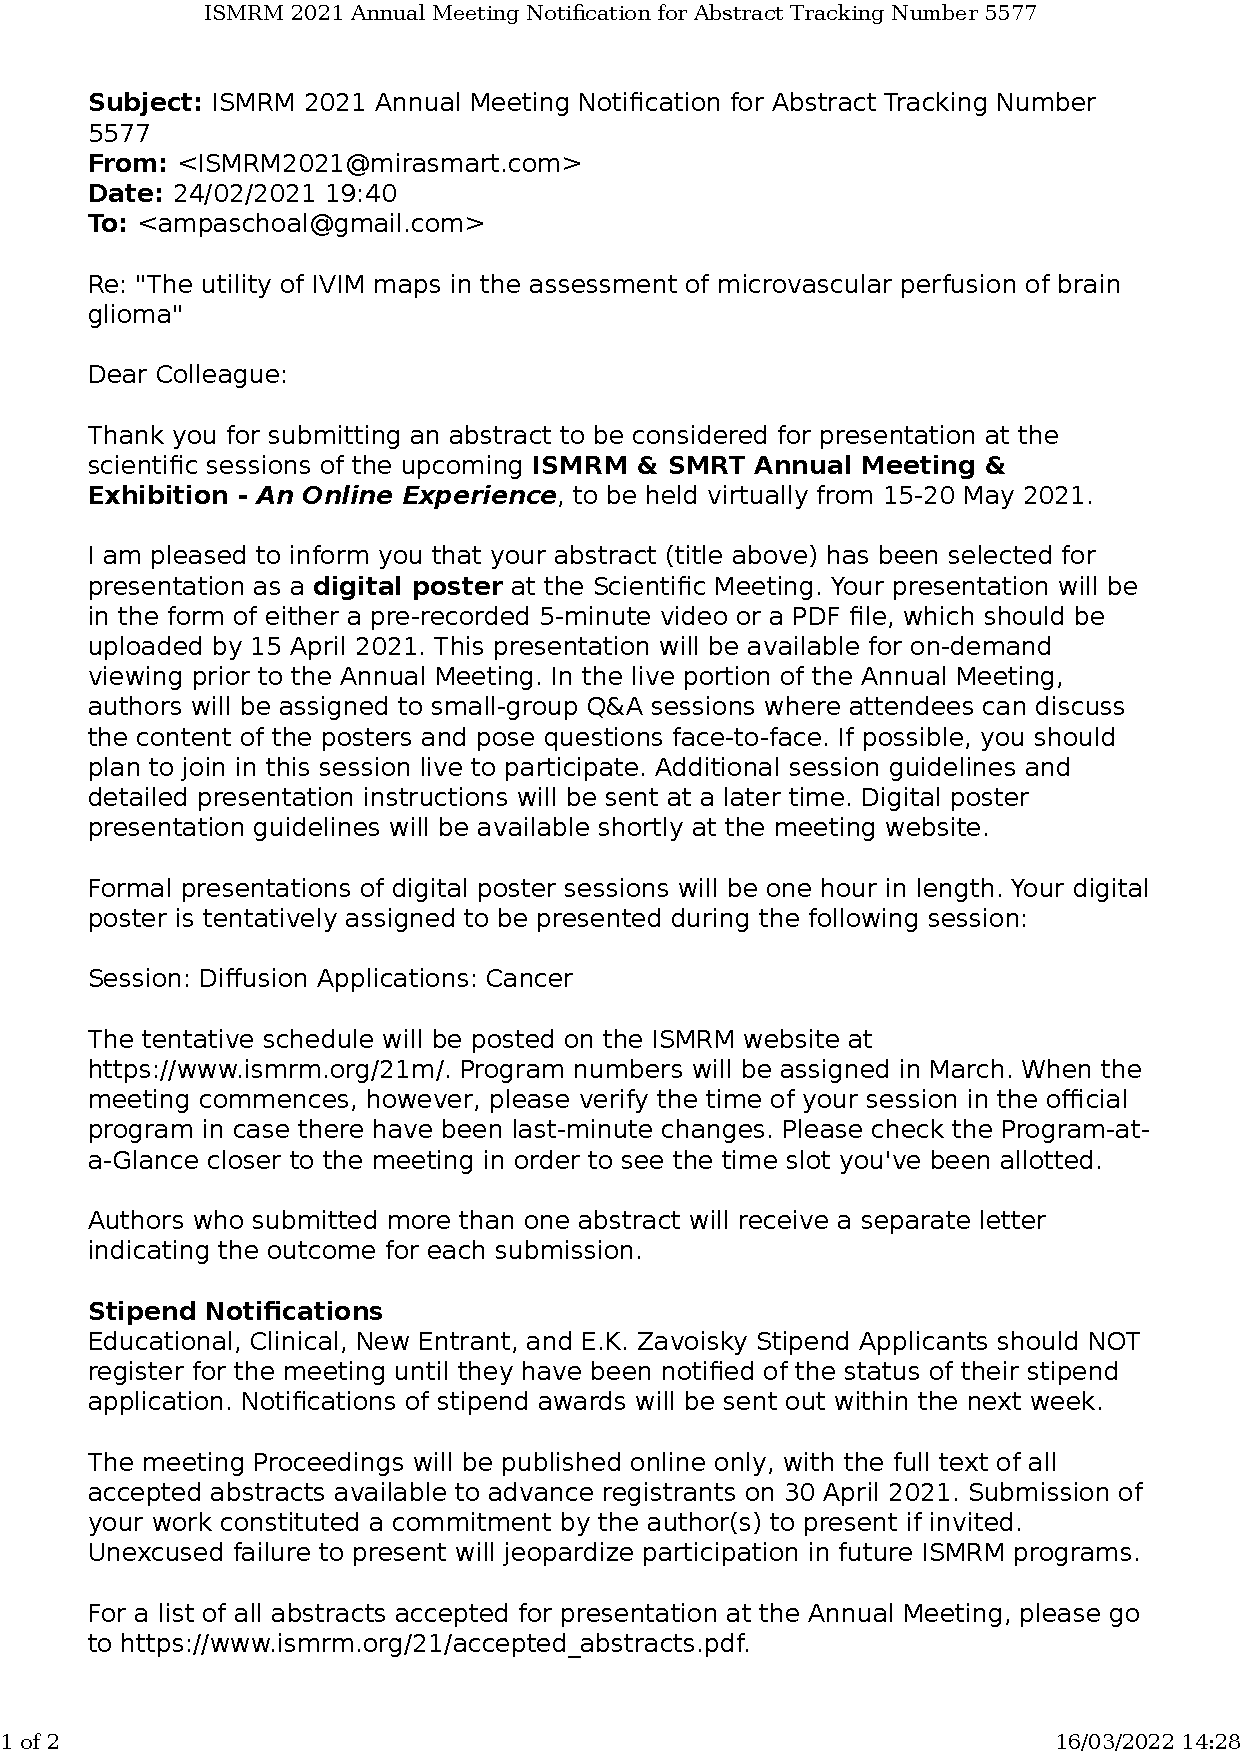
\includepdf[pages=-, scale=1,pagecommand=\thispagestyle{empty}]{\detokenize{Diplomas/AcceptanceISMRM2021_1}}
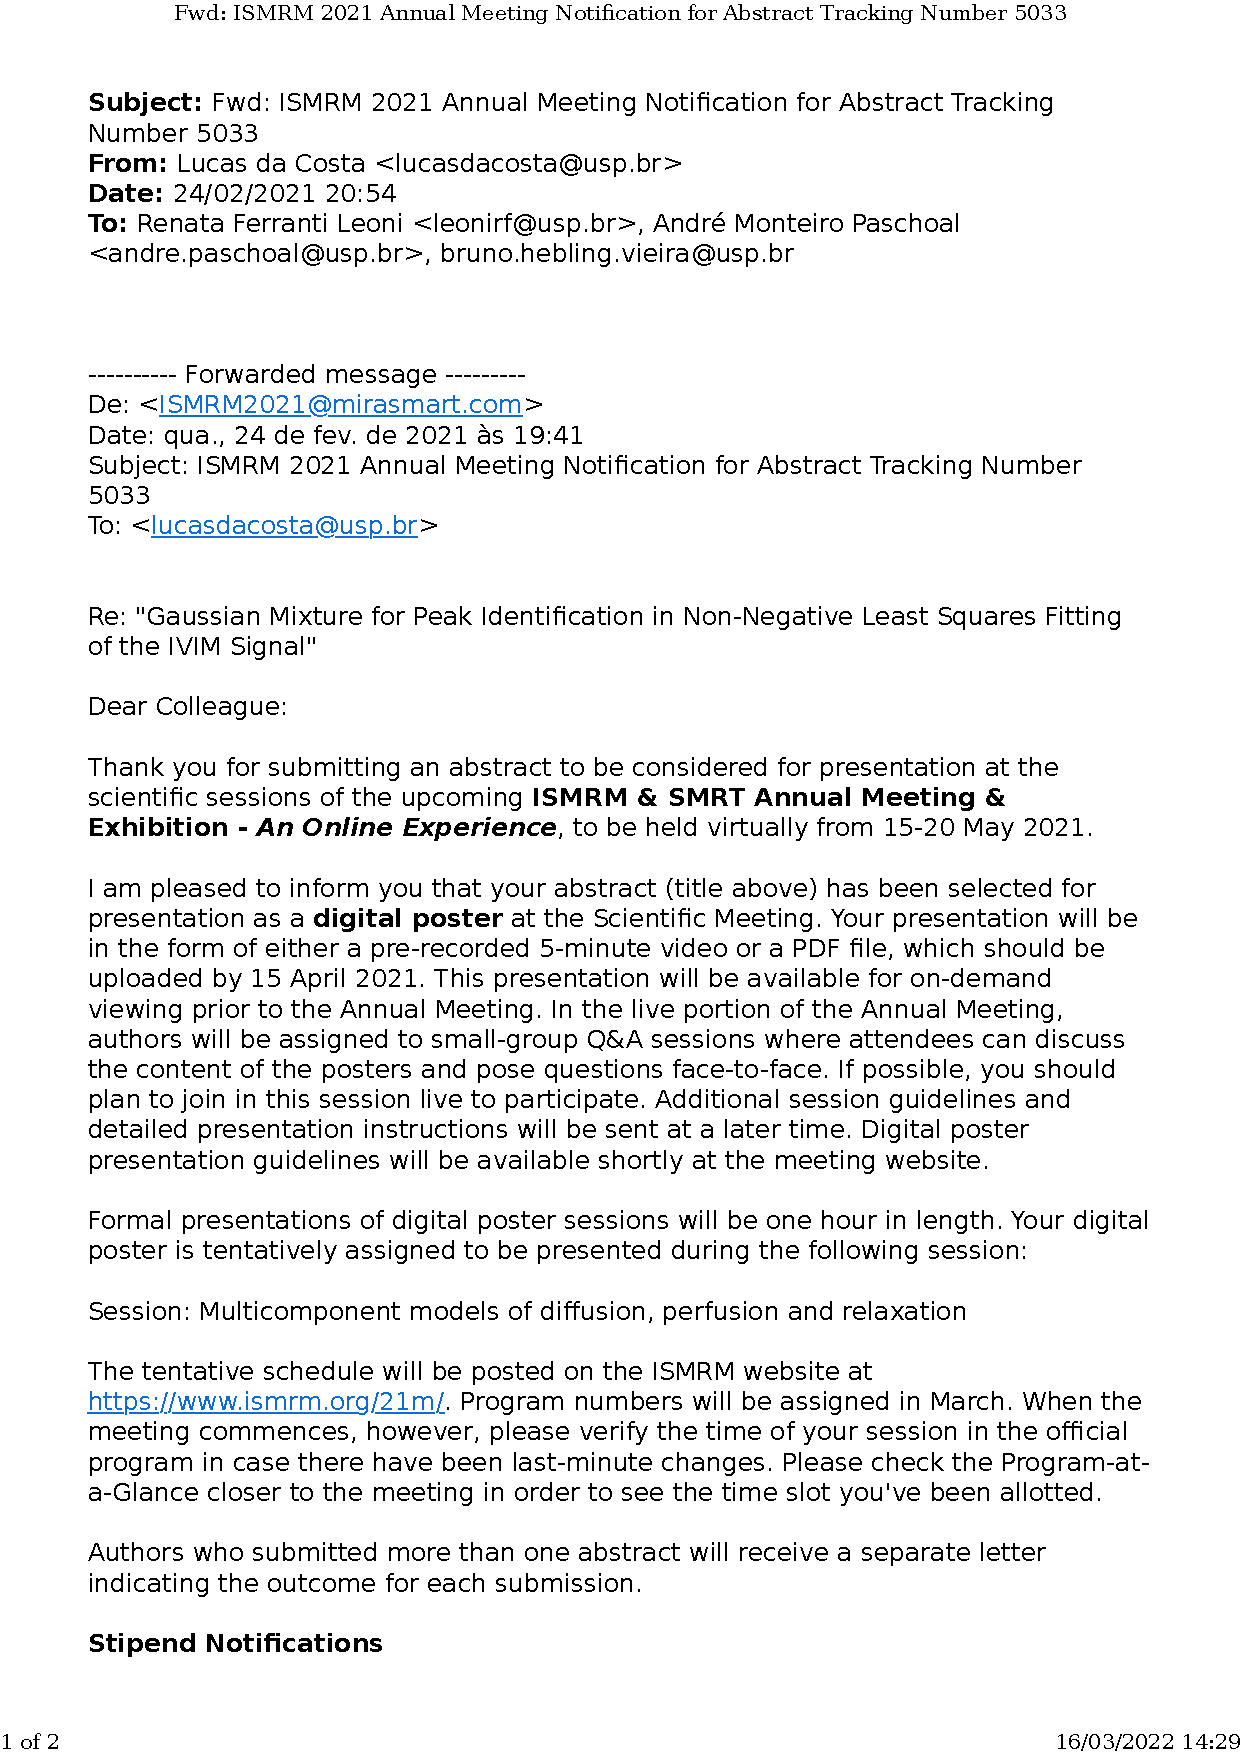
\includepdf[pages=-, scale=1,pagecommand=\thispagestyle{empty}]{\detokenize{Diplomas/AcceptanceISMRM2021_2}}

\newpage
\subsection{Participa\c{c}\~{a}o em Eventos Cient\'{\i}ficos (com apresenta\c{c}\~{a}o de trabalho ou oferecimento de cursos, palestras ou debates}
\label{certificados:JPR2021}
Esta subseção apresenta o comprovante da participação no 
Jornada Paulista de Radiologia 2021 com seus respectivos propósitos. \\
%Obs: Ese congresso não emite certificado de apresentação de trabalhos, apenas de participação no evento.
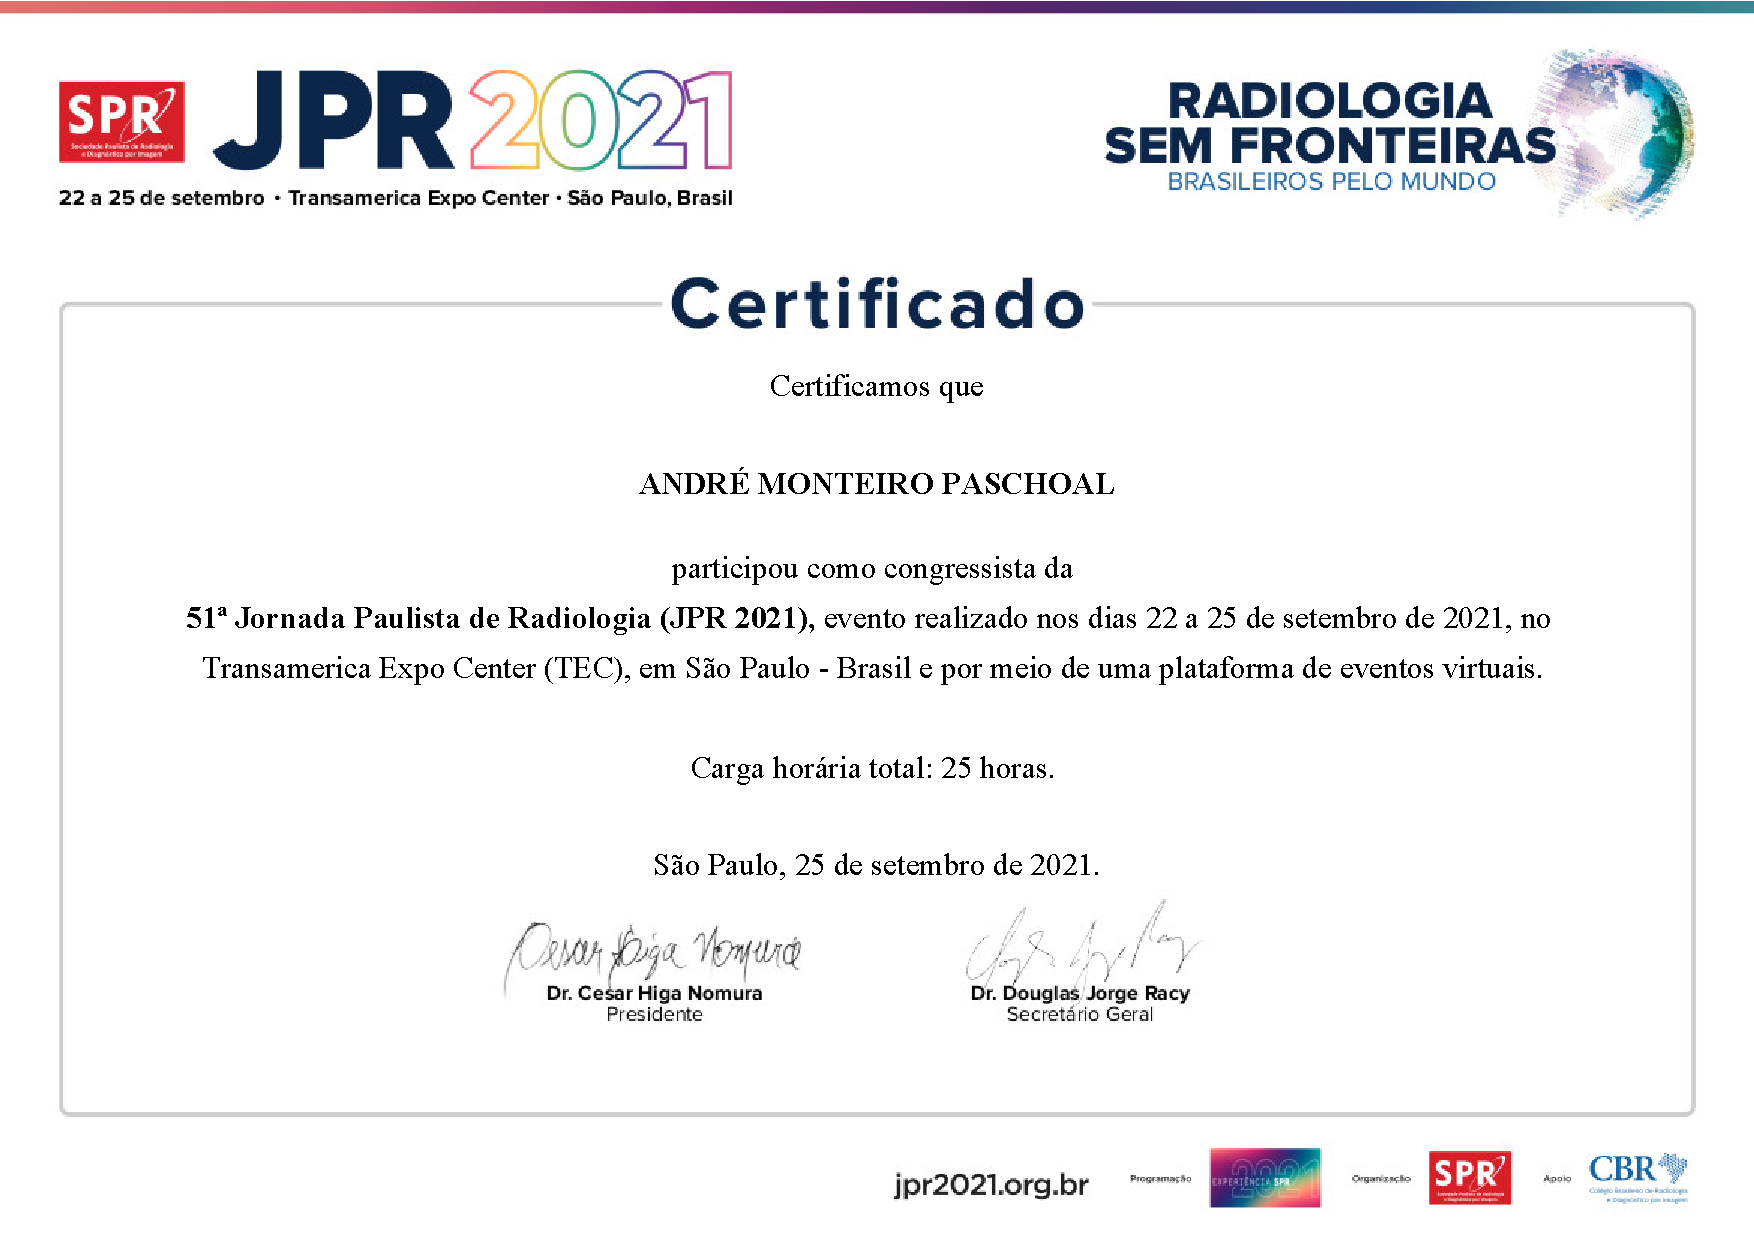
\includepdf[pages=-, scale=1,pagecommand=\thispagestyle{empty}]{\detokenize{Diplomas/JPR2021_1}}
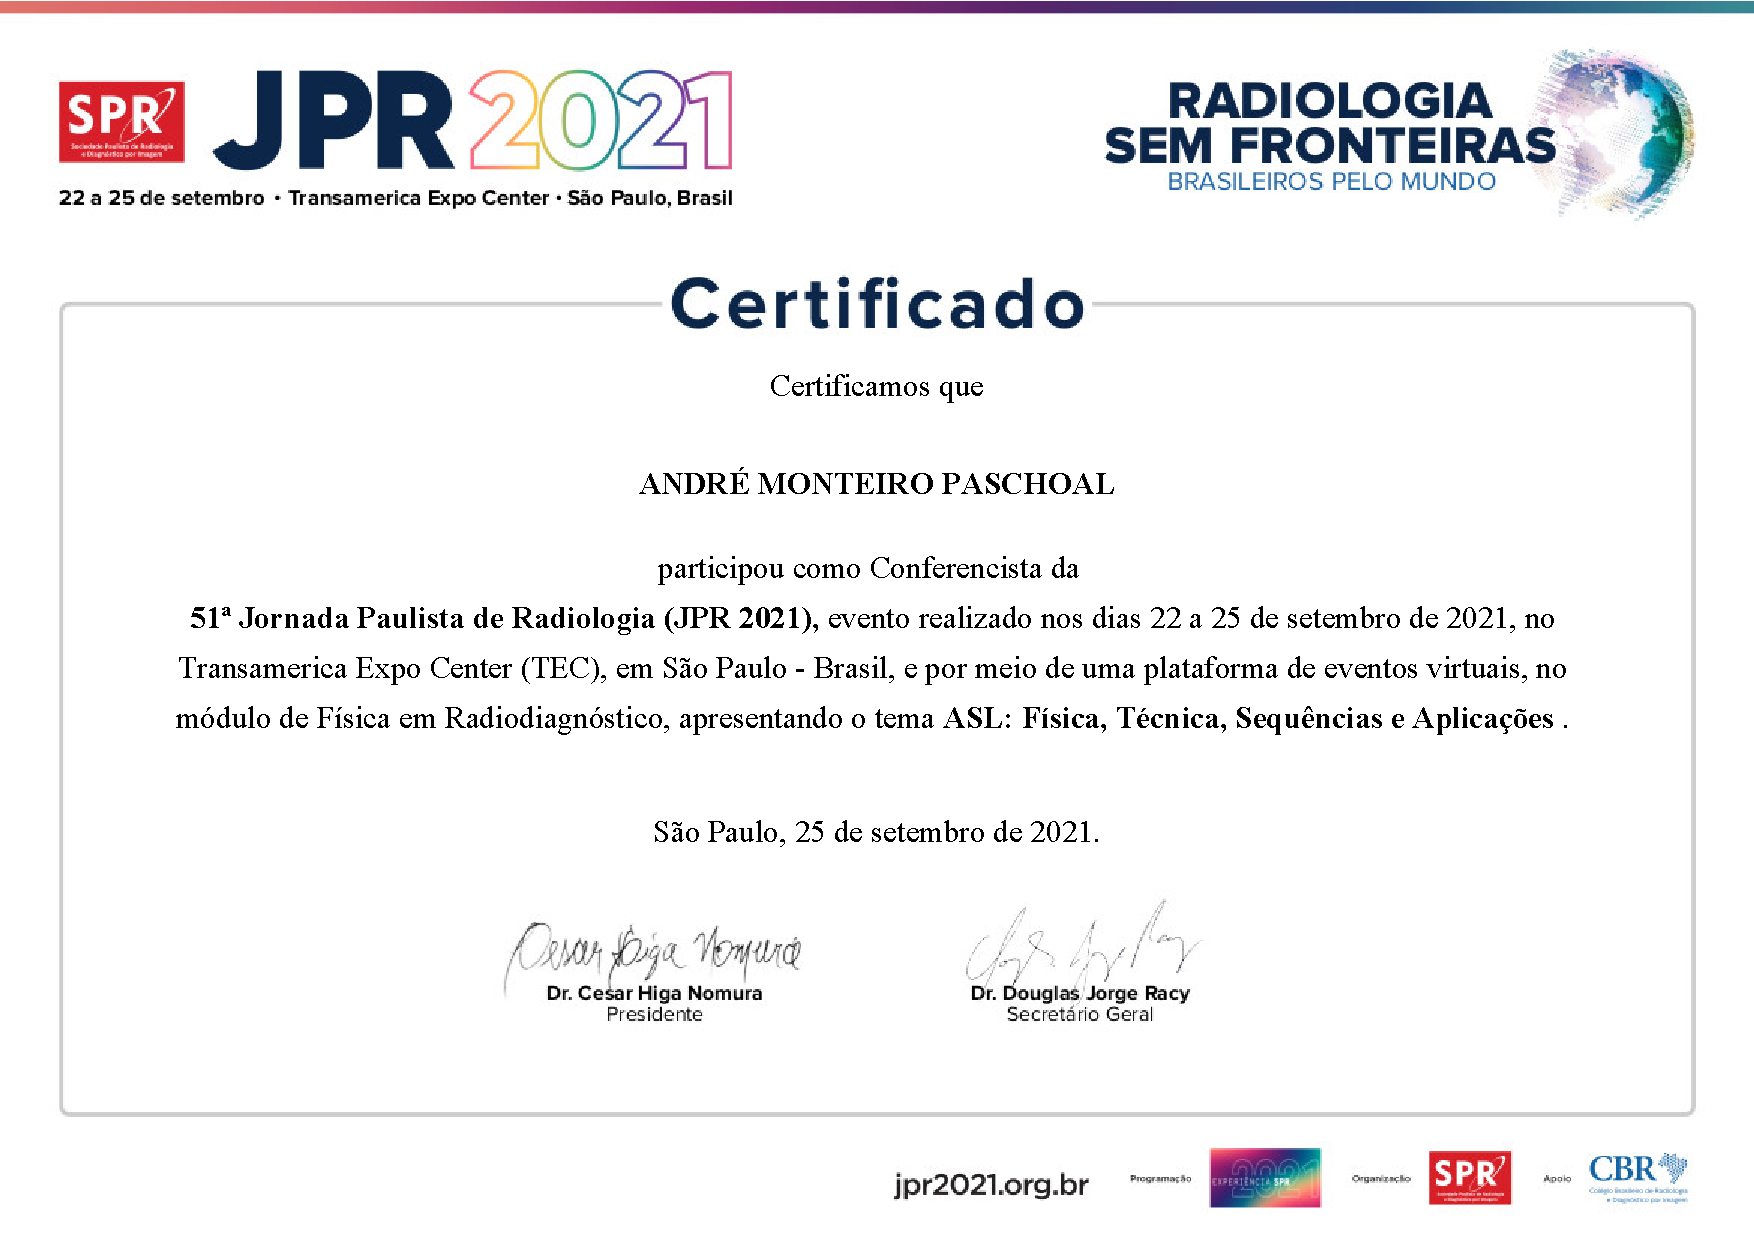
\includepdf[pages=-, scale=1,pagecommand=\thispagestyle{empty}]{\detokenize{Diplomas/JPR2021_2}}

\newpage
\subsection{Participa\c{c}\~{a}o em Eventos Cient\'{\i}ficos (com apresenta\c{c}\~{a}o de trabalho ou oferecimento de cursos, palestras ou debates}
\label{certificados:PWISMRM2022}
Esta subseção apresenta o comprovante da participação no 
ISMRM Perfusion Workshop: from head to toe com seus respectivos propósitos. \\
Obs: Ese congresso não emite certificado de apresentação de trabalhos, apenas de participação no evento.

\includepdf[pages=-, scale=1,pagecommand=\thispagestyle{empty}]{\detokenize{Diplomas/PerfusionWorkshop2022_certificate}}
\includepdf[pages=-, scale=1,pagecommand=\thispagestyle{empty}]{\detokenize{Diplomas/AcceptancePWISMRM2022}}

%---

\newpage
\subsection{Obtenção  de  bolsa  de  estudo  em  instituições de  renome  científico  ou  cultural}
\label{bolsas:mestradoCAPES}
Esta subseção apresenta o comprovante de concessão da bolsa de mestrado CAPES/PROEX.
\includepdf[pages=-, scale=1,pagecommand=\thispagestyle{empty}]{\detokenize{Diplomas/mestradoCAPES}}

\newpage
\subsection{Obtenção  de  bolsa  de  estudo  em  instituições de  renome  científico  ou  cultural}
\label{bolsas:CNPQdoc}
Esta subseção apresenta o comprovante de concessão da bolsa de doutorado CNPq, processo número: 140110/2016-0.
\includepdf[pages=-, scale=1,pagecommand=\thispagestyle{empty}]{\detokenize{Diplomas/CNPq_doutorado}}

\newpage
\subsection{Obtenção  de  bolsa  de  estudo  em  instituições de  renome  científico  ou  cultural}
\label{bolsas:PDSE}
Esta subseção apresenta o comprovante de concessão da bolsa de doutorado sanduíche PDSE-CAPES, processo número: 88881.188976/2018-01.
\includepdf[pages=-, scale=1,pagecommand=\thispagestyle{empty}]{\detokenize{Diplomas/Carta de Concessão PDSE}}

\newpage
\subsection{Obtenção  de  bolsa  de  estudo  em  instituições de  renome  científico  ou  cultural}
\label{bolsas:PDJ}
Esta subseção apresenta o comprovante de concessão da bolsa de pós-doutorado junior PDJ-CNPq, processo número:  151245/2019-3.
\includepdf[pages=-, scale=1,pagecommand=\thispagestyle{empty}]{\detokenize{Diplomas/termoPDJ}}

\newpage
\subsection{Obtenção  de  bolsa  de  estudo  em  instituições de  renome  científico  ou  cultural}
\label{bolsas:TTV}
Esta subseção apresenta o comprovante de concessão da bolsa FAPESP de treinamento técnico nível V, processo número:  2020/13586-7.
\includepdf[pages=-, scale=1,pagecommand=\thispagestyle{empty}]{\detokenize{Diplomas/FAPESP_TTV}}

%---

\newpage
\subsection{Autoria de artigos completos publicados em anais de congresso, em jornais e revistas de circulação nacional e internacional na sua área}
\label{certificados:OHBM2015}
Esta subseção apresenta o comprovante da autoria do resumo publicado em anais do congresso Organization for Human Brain Mapping, 2015.
\includepdf[pages=-, scale=1,pagecommand=\thispagestyle{empty}]{\detokenize{Diplomas/AcceptanceOHBM2015}}

\newpage
\subsection{Autoria de artigos completos publicados em anais de congresso, em jornais e revistas de circulação nacional e internacional na sua área}
\label{certificados:CBFM2019}
Esta subseção apresenta o comprovante da autoria do resumo publicado em anais do congresso Brasileiro de Física Médica, 2019.
\includepdf[pages=-, scale=1,pagecommand=\thispagestyle{empty}]{\detokenize{Diplomas/AceiteCBFM2019}}

\newpage
\subsection{Autoria de artigos completos publicados em anais de congresso, em jornais e revistas de circulação nacional e internacional na sua área}
\label{certificados:ESMRMB2019}
Esta subseção apresenta o comprovante da autoria do resumo publicado em anais do congresso internacional ESMRMB 2019.
\includepdf[pages=-, scale=1,pagecommand=\thispagestyle{empty}]{\detokenize{Diplomas/AcceptanceESMRMB2019}}

%---

\newpage
\subsection{Autoria de artigos completos publicados em jornais e revistas de circulação nacional e internacional na sua área}
\label{artigos:RBFM2013}
Esta subseção apresenta o comprovante da autoria do resumo publicado em anais do congresso Brasileiro de Física Médica, 2019.
\includepdf[pages=-, scale=1,pagecommand=\thispagestyle{empty}]{\detokenize{docs/PaivaRBFM2013}}

\newpage
\subsection{Autoria de artigos completos publicados em jornais e revistas de circulação nacional e internacional na sua área}
\label{artigos:MRI2018}
Esta subseção apresenta o comprovante da autoria do artigo publicado na revista nacional \textit{Revista Brasileira de Física Médica} no ano de 2013.
\includepdf[pages=-, scale=1,pagecommand=\thispagestyle{empty}]{\detokenize{docs/silvamri2018}}

\newpage
\subsection{Autoria de artigos completos publicados em jornais e revistas de circulação nacional e internacional na sua área}
\label{artigos:NICLIN2018}
Esta subseção apresenta o comprovante da autoria do artigo publicado na revista internacional \textit{Neuroimage: clinical} no ano de 2018.
\includepdf[pages=-, scale=1,pagecommand=\thispagestyle{empty}]{\detokenize{docs/Paschoal_NeuroImageClin2018}}

\newpage
\subsection{Autoria de artigos completos publicados em jornais e revistas de circulação nacional e internacional na sua área}
\label{artigos:CONCEPTS2019}
Esta subseção apresenta o comprovante da autoria do artigo publicado na revista internacional \textit{Concepts in Magnetic Resonance Part A} no ano de 2019.
\includepdf[pages=-, scale=1,pagecommand=\thispagestyle{empty}]{\detokenize{docs/Paschoal_ConceptsPartA2019}}

\newpage
\subsection{Autoria de artigos completos publicados em jornais e revistas de circulação nacional e internacional na sua área}
\label{artigos:MAGMA2020}
Esta subseção apresenta o comprovante da autoria do artigo publicado na revista internacional \textit{Magnetic Resonance Materials in Physics, Biology and Medicine} no ano de 2020.
\includepdf[pages=-, scale=1,pagecommand=\thispagestyle{empty}]{\detokenize{docs/Paschoal2020_Article_ContrastOptimizationInArterial}}

\newpage
\subsection{Autoria de artigos completos publicados em jornais e revistas de circulação nacional e internacional na sua área}
\label{artigos:MRM2021}
Esta subseção apresenta o comprovante da autoria do artigo publicado na revista internacional \textit{Magnetic Resonance in Medicine} no ano de 2021.
\includepdf[pages=-, scale=1,pagecommand=\thispagestyle{empty}]{\detokenize{docs/mrm.28807}}

\newpage
\subsection{Autoria de artigos completos publicados em jornais e revistas de circulação nacional e internacional na sua área}
\label{artigos:JNE2021}
Esta subseção apresenta o comprovante da autoria do artigo publicado na revista internacional \textit{Journal of Neural Engineering} no ano de 2021.
\includepdf[pages=-, scale=1,pagecommand=\thispagestyle{empty}]{\detokenize{docs/jne_18_4_046089}}

\newpage
\subsection{Autoria de artigos completos publicados em jornais e revistas de circulação nacional e internacional na sua área}
\label{artigos:JMRI2021}
Esta subseção apresenta o comprovante da autoria do artigo publicado na revista internacional \textit{Journal of Magnetic Resonance Imaging} no ano de 2021.
\includepdf[pages=-, scale=1,pagecommand=\thispagestyle{empty}]{\detokenize{docs/jmri.27899}}

\newpage
\subsection{Autoria de artigos completos publicados em jornais e revistas de circulação nacional e internacional na sua área}
\label{artigos:MAGMA2021}
Esta subseção apresenta o comprovante da autoria do artigo publicado na revista internacional \textit{Magnetic Resonance Materials in Physics, Biology and Medicine} no ano de 2021.
\includepdf[pages=-, scale=1,pagecommand=\thispagestyle{empty}]{\detokenize{docs/Paschoal2022_Article_FeasibilityOfIntravoxelIncoher}}

\newpage
\subsection{Autoria de artigos completos publicados em jornais e revistas de circulação nacional e internacional na sua área}
\label{artigos:NMRBiomed2022_2}
Esta subseção apresenta o comprovante da autoria do artigo publicado na revista internacional \textit{NMR in Biomedicine} no ano de 2022.
\includepdf[pages=-, scale=1,pagecommand=\thispagestyle{empty}]{\detokenize{docs/NBM-22-0068}}

\newpage
\subsection{Autoria de resumo aceito para apresentação em congresso, em jornais e revistas de circulação nacional e internacional na sua área}
\label{certificados:ISMRM2022_1}
Esta subseção apresenta o comprovante de aceite de resumo a ser apresentado no congresso internacional ISMRM 2022.
\includepdf[pages=-, scale=1,pagecommand=\thispagestyle{empty}]{\detokenize{Diplomas/Acceptance_ISMRM2022_1}}
\includepdf[pages=-, scale=1,pagecommand=\thispagestyle{empty}]{\detokenize{docs/ISMRM2022_MS}}

\newpage
\subsection{Autoria de resumo aceito para apresentação em congresso, em jornais e revistas de circulação nacional e internacional na sua área}
\label{certificados:ISMRM2022_2}
Esta subseção apresenta o comprovante de aceite de resumo a ser apresentado no congresso internacional ISMRM 2022.
\includepdf[pages=-, scale=1,pagecommand=\thispagestyle{empty}]{\detokenize{Diplomas/Acceptance_ISMRM2022_2}}
\includepdf[pages=-, scale=1,pagecommand=\thispagestyle{empty}]{\detokenize{docs/ISMRM2022_OSIPI}}

\newpage
\subsection{Autoria de resumo aceito para apresentação em congresso, em jornais e revistas de circulação nacional e internacional na sua área}
\label{certificados:BRAINN2022}
Esta subseção apresenta o comprovante de aceite de resumo a ser apresentado no congresso internacional 8th BRAINN Congress 2022.
\includepdf[pages=-, scale=1,pagecommand=\thispagestyle{empty}]{\detokenize{Diplomas/Acceptance_BRAINN2022}}
\includepdf[pages=-, scale=1,pagecommand=\thispagestyle{empty}]{\detokenize{docs/BRAIN2022}}

\newpage
\subsection{Autoria de resumo aceito para apresentação em congresso, em jornais e revistas de circulação nacional e internacional na sua área}
\label{certificados:JPR2022}
Esta subseção apresenta o comprovante de participação em palestra a ser apresentada no congresso Jornada Paulista de Radiologia 2022.
\includepdf[pages=-, scale=1,pagecommand=\thispagestyle{empty}]{\detokenize{Diplomas/JPR2022}}

%---

\newpage
\subsection{Atividades de docência}
\label{aulas:EEP}
Esta subseção apresenta o certificado de atividades como docente no curso de Especialização em Ressonância Magnética para Biomédicos e Tecnólogos pela Escola de 
Educação Permanente do Hospital das Clínicas da Faculdade de Medicina da Universidade de São Paulo nos anos de 2021 e 2022, ministrando as disciplinas de física básica e física avançada.
\includepdf[pages=-, scale=1,pagecommand=\thispagestyle{empty}]{\detokenize{Diplomas/aulasEEP}}

\newpage
\subsection{Monitorias para disciplinas de graduação}
\label{monitorias:IFSC}
Esta subseção apresenta o comprovante de Monitoria para alunos de graduação.
\includepdf[pages=-, scale=1,pagecommand=\thispagestyle{empty}]{\detokenize{Diplomas/MonitoriaIFSC}}

\newpage
\subsection{Monitorias para disciplinas de graduação}
\label{monitorias:FFCLRP}
Esta subseção apresenta o comprovante de Monitoria para alunos de graduação.
\includepdf[pages=-, scale=1,pagecommand=\thispagestyle{empty}]{\detokenize{Diplomas/monitoriaPIM_2017_1FFCLRP}}

\newpage
\subsection{Monitorias para disciplinas de graduação}
\label{monitorias:PAE1}
Esta subseção apresenta o comprovante de Monitoria para alunos de graduação.
\includepdf[pages=-, scale=1,pagecommand=\thispagestyle{empty}]{\detokenize{Diplomas/monitoriaPAE_2017_2FFCLRP}}

\newpage
\subsection{Monitorias para disciplinas de graduação}
\label{monitorias:PAE2}
Esta subseção apresenta o comprovante de Monitoria para alunos de graduação.
\includepdf[pages=-, scale=1,pagecommand=\thispagestyle{empty}]{\detokenize{Diplomas/monitoriaPAE_2019_2FFCLRP}}

%---

\newpage
\subsection{Membro de Comissão Avaliadora}
\label{avaliador:SIICUSP2019}
Esta subseção apresenta o comprovante de participação em comissão avaliadora de eventos.
\includepdf[pages=-, scale=1,pagecommand=\thispagestyle{empty}]{\detokenize{Diplomas/certificado_siicusp}}

\newpage
\subsection{Membro de Comissão Avaliadora}
\label{avaliador:SFM2019}
Esta subseção apresenta o comprovante de participação em comissão avaliadora de eventos.
\includepdf[pages=-, scale=1,pagecommand=\thispagestyle{empty}]{\detokenize{Diplomas/certificadoAvaliador_SFM2019}}

\newpage
\subsection{Membro de Comissão Avaliadora}
\label{avaliador:SIICUSP2020}
Esta subseção apresenta o comprovante de participação em comissão avaliadora de eventos.
\includepdf[pages=-, scale=1,pagecommand=\thispagestyle{empty}]{\detokenize{Diplomas/SIICUSP2020}}

%---

%%%%%%%%%%%%%%%%%%%%%%%%%%%%%%%%%%%%%%%%%%%%%%%%%%%%%%%%%%%%%%%%%%%%%%%%%%%%%%%
% Subgrupo 3.2 - Coordenação de Eventos e Conferencista
%%%%%%%%%%%%%%%%%%%%%%%%%%%%%%%%%%%%%%%%%%%%%%%%%%%%%%%%%%%%%%%%%%%%%%%%%%%%%%%

%\newpage
%\subsection{Comiss\~{a}o Organizadora de Eventos Internacional, Nacional, Regional ou Local}
%\label{reviewer:2015-sbcars}
%Esta subseção apresenta o comprovante de Comiss\~{a}o Organizadora do 9th Brazilian Symposium on Software Components, Architectures and Reuse (SBCARS 2015).
%\includepdf[pages=-, scale=1,pagecommand=\thispagestyle{empty}]{\detokenize{GRUPO 3/Sub-Grupo 32/Comprovante Fake}}

%%%%%%%%%%%%%%%%%%%%%%%%%%%%%%%%%%%%%%%%%%%%%%%%%%%%%%%%%%%%%%%%%%%%%%%%%%%%%%%
% Grupo 4: Atividades de Forma\c{c}\~{a}o e Capacita\c{c}\~{a}o Acad\^{e}mica
%%%%%%%%%%%%%%%%%%%%%%%%%%%%%%%%%%%%%%%%%%%%%%%%%%%%%%%%%%%%%%%%%%%%%%%%%%%%%%%

\newpage
\subsection{Comiss\~{a}o Organizadora de Eventos Internacional, Nacional, Regional ou Local}
\label{organizacao:inbrain}
Esta subseção apresenta o comprovante de Participação de Comissão Organizadora de Eventos Nacionais e Internacionais.
\includepdf[pages=-, scale=1,pagecommand=\thispagestyle{empty}]{\detokenize{Diplomas/InBrainWorkshop_organizacao}}

\newpage
\subsection{Comiss\~{a}o Organizadora de Eventos Internacional, Nacional, Regional ou Local}
\label{organizacao:eifamb}
Esta subseção apresenta o comprovante de Participação de Comissão Organizadora de Eventos Nacionais e Internacionais.
\includepdf[pages=-, scale=1,pagecommand=\thispagestyle{empty}]{\detokenize{Diplomas/EIFAMB2018_CO_AndréMonteiroPaschoal}}

%------------------------------------------------------------------------------
%%%%%%%%%%%%%%%%%%%%%%%%%%%%%%%%%%%%%%%%%%%%%%%%%%%%%%%%%%%%%%%%%%%%%%%%%%%%%%%
% \newpage
% \subsection{Portaria de Progressão}
% \label{app:2014-portaria-progressao}
% \includepdf[pages=-, scale=1,pagecommand=\thispagestyle{empty}]{\detokenize{GRUPO 1/20141205_Portaria-de-Progressao-Funcional_5929-2014.pdf}}


\end{document}

%%% EOF
